%%%%%%%%%%%%%%%%%%%%%%%%%%%%%%%%%%%%%%%%%%%%%%%%%%%%%%%%%%%%%%%%%
% Tese de Doutorado / Dept Fisica, CFM, UFSC                    %
% Andre@UFSC - 2014                                             %
%%%%%%%%%%%%%%%%%%%%%%%%%%%%%%%%%%%%%%%%%%%%%%%%%%%%%%%%%%%%%%%%%
\documentclass[final]{nathesis_A5}

\begin{document}

\frontmatter
  \pagenumbering{arabic}
  %%%%%%%%%%%%%%%%%%%%%%%%%%%%%%%%%%%%%%%%%%%%%%%%%%%%%%%%%%%%%%%%%
% Dissertacao de Mestrado / Dept Fisica, CFM, UFSC              %
% Andre@UFSC - 2011                                             %
%%%%%%%%%%%%%%%%%%%%%%%%%%%%%%%%%%%%%%%%%%%%%%%%%%%%%%%%%%%%%%%%%


%***************************************************************%
%                                                               %
%                            CAPA                               %
%                                                               %
%***************************************************************%

\institution{Universidade Federal de Santa Catarina \\
Centro de Ciências Físicas e Matemáticas \\
Programa de Pós-Graduação em Física}

\thesistitle{Exame de qualificação de doutorado: \\ 
Novos passos na síntese espectral de galáxias}

\thesisauthor{André Luiz de Amorim}

\supervisor{Prof.\ Dr.\ Roberto Cid Fernandes Jr.}

\cosupervisor{Mister M.}

\comments{}

\place{Florianópolis (SC)}
\thesisdate{\today}

\maketitle
\clearpage
  %%%%%%%%%%%%%%%%%%%%%%%%%%%%%%%%%%%%%%%%%%%%%%%%%%%%%%%%%%%%%%%%%
% Dissertacao de Mestrado / Dept Fisica, CFM, UFSC              %
% Andre@UFSC - 2011                                             %
%%%%%%%%%%%%%%%%%%%%%%%%%%%%%%%%%%%%%%%%%%%%%%%%%%%%%%%%%%%%%%%%%


%***************************************************************%
%                                                               %
%                          Dedicatória                          %
%                                                               %
%***************************************************************%

\thispagestyle{plain}

\

\vfill

\begin{flushright}
\hfill \textit{Para Marilize e nosso pequeno mais-que-tudo.}
\end{flushright}

\vspace*{1cm}

\thispagestyle{empty}
\cleardoublepage
\thispagestyle{empty}
\clearpage
  %%%%%%%%%%%%%%%%%%%%%%%%%%%%%%%%%%%%%%%%%%%%%%%%%%%%%%%%%%%%%%%%%
% Dissertacao de Mestrado / Dept Fisica, CFM, UFSC              %
% Andre@UFSC - 2011                                             %
%%%%%%%%%%%%%%%%%%%%%%%%%%%%%%%%%%%%%%%%%%%%%%%%%%%%%%%%%%%%%%%%%


%***************************************************************%
%                                                               %
%                        Agradecimentos                         %
%                                                               %
%***************************************************************%

\chapter*{Agradecimentos}

Agradece.

Não esquecer CAPES, INCT-A, Ciências sem Fronteiras, IAA, CALIFA.

% End of Acknowledgments
\clearpage
  %%%%%%%%%%%%%%%%%%%%%%%%%%%%%%%%%%%%%%%%%%%%%%%%%%%%%%%%%%%%%%%%%
% Dissertacao de Mestrado / Dept Fisica, CFM, UFSC              %
% Andre@UFSC - 2011                                             %
%%%%%%%%%%%%%%%%%%%%%%%%%%%%%%%%%%%%%%%%%%%%%%%%%%%%%%%%%%%%%%%%%

%***************************************************************%
%                                                               %
%                          Resumo                               %
%                                                               %
%***************************************************************%

\begin{abstract}[Resumo]

A figura a seguir resume esta tese.

\begin{center}
\includegraphics[width=0.7\textwidth]{figuras/lmp}
\end{center}

\end{abstract}

% End of resumo
\clearpage
  %%%%%%%%%%%%%%%%%%%%%%%%%%%%%%%%%%%%%%%%%%%%%%%%%%%%%%%%%%%%%%%%%
% Dissertacao de Mestrado / Dept Fisica, CFM, UFSC              %
% Andre@UFSC - 2011                                             %
%%%%%%%%%%%%%%%%%%%%%%%%%%%%%%%%%%%%%%%%%%%%%%%%%%%%%%%%%%%%%%%%%

%***************************************************************%
%                                                               %
%                          Abstract                             %
%                                                               %
%***************************************************************%

\begin{abstract}

In this work we developed some tools to work with Integral Field Spectroscopy
(IFS) spectra from the CALIFA survey. The spectra from the spaxels are
preprocessed, and then analyzed using the software \starlight. One of the main
tools discussed here, PyCASSO, organizes the output from \starlight into
datacubes of stellar population synthesis products. It also allows for
interactive exploratory programming, giving easy access to the multi-dimensional
data.

Using these tools, we developed a method for recovering and analysing the
stellar populations of the different morphological components of galaxies using
IFS data. Using the software Imfit, wrapped in Python, we perform the
decomposition of a sample of 43 candidate S0 galaxies from the CALIFA Survey
into a Sérsic bulge and an exponential disk. The decomposition is made
wavelength-wise, so that at the end we get the bulge and disk spectra for each
pixel. A good PSF measurement is critical to this process, so we perform a
characterization of the PSF using the calibration stars from the survey. The
morphological parameters ($r_e$, $n$, P.A. and $\epsilon$ for bulge, $h$, P.A.
and $\epsilon$ for disk) in most cases depends linearly on the wavelength, in
average, but their behavior in each $\lambda$ are not yet fully unerstood.
Using the decomposed spectra from the 9 best decompositions from the sample we
apply a stellar population synthesis using \starlight, in order to recover the
stellar populations of bulge and disk. Only two of those galaxies produced good
\starlight fits, CALIFA 0592 (NGC 4874) and CALIFA 0858 (UGC 10905). In both
cases we recover an older and lower metallic bulge and an younger and more
metallic disk (in comparison to the whole galaxy). The stellar synthesis
produces more robust results using the integrated spectra. The spatially
resolved spectra from bulge and disk seem to have artifacts that get interpreted
as dust, among other things, thus leading to wrong results.


\end{abstract}

% End of abstract



\clearpage
  \tableofcontents\clearpage
  \listoffigures\clearpage
  \listoftables\clearpage

\mainmatter*

  % Introdução
  %%%%%%%%%%%%%%%%%%%%%%%%%%%%%%%%%%%%%%%%%%%%%%%%%%%%%%%%%%%%%%%%%
% Qualificacao de Doutorado / Dept Fisica, CFM, UFSC            %
% Andre@UFSC - 2013                                             %
%%%%%%%%%%%%%%%%%%%%%%%%%%%%%%%%%%%%%%%%%%%%%%%%%%%%%%%%%%%%%%%%%

%:::::::::::::::::::::::::::::::::::::::::::::::::::::::::::::::%
%                                                               %
%                          Capítulo 1                           %
%                                                               %
%:::::::::::::::::::::::::::::::::::::::::::::::::::::::::::::::%

%***************************************************************%
%                                                               %
%                         Introdução                            %
%                                                               %
%***************************************************************%

\chapter{Introdução}
\label{sec:intro}

%***************************************************************%
%                                                               %
%                         Intro - IFS                           %
%                                                               %
%***************************************************************%

\section{Espectroscopia de campo integral}

Na última década presenciamos uma proliferação de surveys de imageamento e
espectroscopia. Surveys como o SDSS \citep{York2000}, ALHAMBRA \citep{Moles2008}
e COSMOS \citep{Scoville2007}, para citar alguns exemplos, permitem explorar a
distribuição espectral de energia (SED\footnote{\em Spectral Energy
Distribution.}) de centenas de milhares a milhões de galáxias.
Entretanto, da forma como estes surveys são executados, há sempre um compromisso
entre a resolução espacial e a espectral. As imagens obtidas pelo SDSS têm um
boa resolução espacial, mas mapeiam a SED de forma grosseira, com apenas $5$
filtros de banda larga ($ugriz$). Já os espectros obtidos pelo mesmo survey
possuem uma excelente resolução e cobertura espectral, mas obtém o espectro
integrado da região central das galáxias.

O melhor dos dois mundos pode ser alcançado com instrumentos que fazem
espectroscopia de campo integral (IFS\footnote{\em Integral Field
Spectroscopy.}). Instrumentos que realizam este tipo de espectroscopia consistem
em geral de um amontoado de fibras óticas, as quais alimentam um espectrógrafo
comum. Assim, depois de um processo relativamente complicado de redução de
dados, obtém-se espectros espacialmente resolvidos com uma boa resolução
espectral e espacial. O survey CALIFA ({\em Calar Alto Legacy Integral Field
Area survey\footnote{\url{http://www.caha.es/CALIFA/}}}) está utilizando o
instrumento PMAS/PPAK do observatório Calar Alto para obter IFS de $600$
galáxias \citep{Sanchez2012}.
Destas, $100$ já estão disponíveis no primeiro {\em Data Release}
\citep[DR1]{Husemann2013}, afirmando o caráter de legado deste survey.

Quando completado, o CALIFA terá obtido da ordem de $10^6$ espectros, quase o
mesmo que o SDSS. Porém, este não será apenas mais um survey espectroscópico. A
riqueza do CALIFA está nas informações espacialmente resolvidas, em uma amostra
representativa do universo local ($0.005 < z < 0.03$, limitada em diâmetro
angular) cobrindo a distribuição de galáxias no diagrama cor--magnitude da nuvem
azul à sequência vermelha, amostrando galáxias todos os tipos morfológicos
(espirais, elípticas, irregulares e até mesmo alguns sistemas em interação).


%***************************************************************%
%                                                               %
%                Intro - Stellar synthesis of IFS               %
%                                                               %
%***************************************************************%

\section{Síntese de população estelar espacialmente resolvida}
\label{sec:Intro:Sintese}

Os espectros espacialmente resolvidos do CALIFA podem ser descritos como um cubo
de dados, com as duas primeiras dimensões sendo a posição $x$ e $y$ (ascensão
reta e declinação) e a terceira sendo o comprimento de onda. Nestes cubos,
planos com comprimento de onda constante são imagens, enquanto ``fatias''
definidas por um par $(x, y)$ constante são espectros. Pode-se tratar estes
espectros individualmente, embora na verdade, nos cubos do CALIFA os pixels
vizinhos estão correlacionados devido ao {\em seeing} do céu e ao processo de
observação. Há a queda na relação sinal/ruído (S/N) nas regiões mais
afastadas do núcleo da galáxia, onde o brilho superficial é muito menor.
Algumas galáxias possuem outros objetos ``intrusos'' que precisam ser
mascarados. Linhas telúricas\footnote{Linhas de absorção causadas pela
atmosfera.} também precisam ser mascaradas. Assim, em geral, é necessário um
preprocessamento visando manter um S/N mínimo e garantir um espectro livre de
contaminação. Para mais detalhes sobre o preprocessamento utilizado neste
trabalho, ler a seção 3 do Apêndice \ref{apendice:PaperResolving1}.

% \TODO: o que nós fazemos?

Um aspecto importante do preprocessamento utilizado é que o cubo de dados é
dividido em zonas de Voronoi, onde regiões com baixo S/N são combinadas formando
efetivamente ``pixels maiores''. Desta forma, o cubo original é transformado
numa matriz de zonas e comprimento de onda, onde fatias de zona constante são
espectros. Com isso, os espectros, e as máscaras e erros que os acompanham,
estão prontos para serem usados pelo próximo passo.

A síntese de população estelar consiste em obter a história de formação estelar
(SFH) de uma galáxia utilizando modelos de população estelar simples (SSP).
Ajusta-se o espectro de uma galáxia como a soma de espectros de SSPs com idades
e composições químicas distintas (levando em conta a atenuação por poeira). O
resultado é um vetor de frações de luz e massa destas SSPs, que podem ser
facilmente convertidos a uma SFH conforme a prescrição de \cite{Asari2007}.
O programa utilizado é o \starlight, desenvolvido por \cite{CidFernandes2005}.

Considerando cada zona como uma galáxia distinta\footnote{O que é razoável, já
que cada pixel corresponde em geral a uma distância de centenas de parsecs,
comportando facilmente vários aglomerados e regiões de formação estelar.},
alimentamos todos os espectros das zonas ao \starlight, obtendo o resultado da
síntese como um arquivo de síntese separado para cada zona. Entretanto, para
visualizar ou mesmo tentar entender estes resultados, é preciso organizar e
converter estes arquivos para um formato mais adequado.


%***************************************************************%
%                                                               %
%                        Intro - PyCASSO                        %
%                                                               %
%***************************************************************%

\section{O nascimento do PyCASSO}

Todo o descrito anteriormente forma o alicerce deste presente trabalho. Da
necessidade de manipular os resultados da síntese dos cubos de dados das
galáxias do CALIFA, nasceu o software PyCASSO.

PyCASSO ({\em Python CALIFA \starlight Synthesis Organizer}) é um software
desenvolvido em Python com o objetivo de gerenciar os dados produzidos pelo
\starlight com base nos dados do CALIFA. O Capítulo \ref{sec:pycasso} apresenta
a documentação do PyCASSO, e em seguida discute os artigos publicados que o
utilizam intensivamente.


%***************************************************************%
%                                                               %
%                      Intro - Decomposicao                     %
%                                                               %
%***************************************************************%

\section{Decomposição morfológica de galáxias}

Como aplicação científica do PyCASSO, o Capítulo \ref{sec:Decomp} trata da
síntese espectral das componentes morfológicas\footnote{As componentes
morfológicas de uma galáxia, tratadas neste trabalho, são o bojo e o disco.} de
uma galáxia. As componentes, são determinadas através de ajuste de perfil de
brilho, para cada comprimento de onda. Assim se obtém um cubo de espectros para
cada componente morfológica.Estes cubos são tratados como galáxias separadas, e
seus espectros são passados pelo \starlight. O resultado são cubos extras de
síntese espectral, os quais podem ser comparados com a síntese da galáxia
original. Este estudo está em progresso no momento, os resultados aqui
apresentados são preliminares.

% End of this chapter

  
  % IFS + CALIFA
  %%%%%%%%%%%%%%%%%%%%%%%%%%%%%%%%%%%%%%%%%%%%%%%%%%%%%%%%%%%%%%%%%
% Tese de Doutorado / Dept Fisica, CFM, UFSC                    %
% Andre@UFSC - 2014                                             %
%%%%%%%%%%%%%%%%%%%%%%%%%%%%%%%%%%%%%%%%%%%%%%%%%%%%%%%%%%%%%%%%%

%:::::::::::::::::::::::::::::::::::::::::::::::::::::::::::::::%
%                                                               %
%                          Capítulo 2                           %
%                                                               %
%:::::::::::::::::::::::::::::::::::::::::::::::::::::::::::::::%

%***************************************************************%
%                                                               %
%                         IFS + CALIFA                          %
%                                                               %
%***************************************************************%

\chapter{Síntese de populações estelares em espectroscopia de campo integral}
\label{sec:ifs}

%***************************************************************%
%                                                               %
%                      O survey CALIFA                          %
%                                                               %
%***************************************************************%

\section{O {\em survey} CALIFA}
\label{sec:ifs:califa}

O {\em Centro Astronómico Hispano Alemán} (CAHA) se localiza na {\em Sierra de
los Filabres}, na Comunidade Autônoma de Andaluzia, Espanha. Ele é operado pelo
{\em Max-Planck-Institut für Astronomie} (MPIA), em Heidelberg, Alemanha, e pelo
{\em Instituto de Astrofísica de Andalucía} (IAA/CSIC), em Granada, Espanha. O
{\em survey} CALIFA foi agraciado com 210 noites pelo Comitê Executivo do Calar
Alto, espalhadas por 6 semestres, iniciando em junho de 2010 (na prática, as
observações se estenderam até o final de 2014). O instrumento utilizado foi a
unidade de campo integral PPAK\footnote{{\em PMAS fiber PAcK}.}
\citep{Kelz2006}, do Espectrógrafo PMAS\footnote{{\em Potsdam Multi-Aperture
Spectrophotometer.}} \citep{Roth2005, Roth2010}, no telescópio de
$3,5\,\mathrm{m}$ do CAHA.

A intenção do {\em survey} é caracterizar a população local de galáxias, que
pode ser resumida nos seguintes aspectos científicos principais
\citep{Sanchez2012}:
\begin{itemize}
  \item Amostra cobrindo uma fração substancial da função de luminosidade.
  \item Amostra grande o suficiente para obter conclusões com uma estatística
  significativa para todas as classes de galáxias do {\em survey}.
  \item Caracterização das galáxias sobre toda a sua extensão, evitando bias de
  abertura.
  \item Determinação de mecanismos de ionização do gás: formação estelar,
  choques, AGN.
  \item Medição de abundâncias de oxigênio e nitrogênio no gás ionizado (regiões
  \HII).
  \item Medição de propriedades de populações estelares: idades, razões
  massa-luminosidade, metalicidades e (de forma limitada) padrões de
  abundâncias.
  \item Medição de cinemática galática em gás em estrelas, campos de velocidade
  para todas as galáxias e dispersão de velocidades para as mais massivas.
\end{itemize}
A arquitetura do {\em survey} foi então desenhada levando em conta os
requerimentos acima, junto com as limitações instrumentais e de tempo
disponível. Ela está descrita nas seções a seguir.

\subsection{Instrumentação}
\label{sec:ifs:instrumentacao}

% FIXME: Rogério - Labels em português.

\begin{figure}
	\includegraphics[width=0.7\textwidth]{figuras/PPAK}
	\caption[Distribuição das fibras no instrumento PMAS/PPAK]
	{Distribuição espacial das fibras e dimensões do IFU do instrumento PMAS/PPAK.
	Círculos brancos representam fibras ativas, e círculos pretos fibras
	espaçadoras, que têm apenas papel estrutural e não obtêm espectros. Os 6
	conjuntos de fibras ao redor do IFU são utilizados para medir o céu. O tamanho
	físico é de $4\,\mathrm{mm}$ e a largura do campo é maior que $1\,\arcs$.
	Retirado de	\citet{Kelz2006}.}
	\label{fig:PPAK}
\end{figure}

À época do início do CALIFA\footnote{Hoje em dia o MUSE
(\url{https://www.eso.org/sci/facilities/develop/instruments/muse.html}) é o
detentor do recorde.}, o PPAK/PMAS era o instrumento de sua classe com o maior
tamanho de campo, $>1\,\mathrm{arcmin}^2$. Ele consiste em um maço de 331 fibras
ópticas cobrindo o campo de observação, direcionado a um espectrógrafo de fenda
longa que espalha a luz sobre um detector CCD\footnote{{\em Charge Coupled
Device}.}.
A Figura \ref{fig:PPAK} ilustra a montagem esquemática do instrumento. Desta
forma, de cada fibra se obtém um espectro. Através de um programa de computador,
os espectros podem ser reorganizados de modo a formar um cubo de dados, onde há
duas dimensões espaciais e uma dimensão espectral.
Todavia, pode-se notar na Figura \ref{fig:PPAK} que as fibras não cobrem
totalmente o campo de observação. Na verdade, apenas em torno de 60\% da luz
proveniente do campo cai dentro das fibras. O restante se perde nos espaços
entre elas. Para mitigar este problema utiliza-se uma técnica chamada {\em
dithering}, observando-se o mesmo campo 3 vezes, a cada vez deslocando o
telescópio uma fração do diâmetro de uma fibra em direções diferentes formando
um triângulo, tal que as 3 exposições cobrem toda a àrea a ser observada. O cubo
de dados é reconstruído utilizando os programas de computador da {\em pipeline}
de observação \citep{Sanchez2012}.

\begin{figure}
	\includegraphics{figuras/DR2_sample_spectra}
	\caption[Exemplos de espectros V500 e V1200 do CALIFA]
	{Espectros V500 e V1200 da galáxia NGC 7625, publicada no DR2 do CALIFA
	\citep{GarciaBenito2015}. Nos painéis superiores são mostradas imagens em
	$4500\,\angstrom$ nas duas configurações. Os espectros referentes aos pontos
	de cores violeta e vermelho, localizados no núcleo, e aos pontos de cores
	verde e laranja, a $12\,\arcs$ do núcleo, são mostrados no painel inferior,
	com as mesmas cores. A linha tracejada mostra o comprimento de onda utilizado
	nas imagens.}
	\label{fig:DR2ExampleSpectra}
\end{figure}

A estratégia inicial do {\em survey} foi observar todos os objetos utilizando
duas configurações diferentes e complementares do instrumento. A primeira
utiliza a grade de difração V500, com resolução $\lambda / \Delta\lambda \approx
850$ em $\lambda = 5000\,\angstrom$ e uma largura a meia altura $\mathrm{FWHM}
\approx 6\,\angstrom$, cobrindo a maior faixa espectral possível, tal que as
linhas \OII e \SII sejam observadas para todos os objetos da amostra.
A segunda utiliza a grade de difração V1200, com resolução $\lambda /
\Delta\lambda \approx 1650$ em $\lambda = 4500\,\angstrom$ e uma largura a meia
altura $\mathrm{FWHM} \approx 2,7\,\angstrom$, cobrindo a faixa azul do
espectro, para incluir a descontinuidade de Balmer, \Hdelta, \Hgamma e
\OIII4363.
Estas duas configurações são chamadas daqui em diante de V500 e V1200
respectivamente. A principal motivação para as observações com a V1200 é medir a
cinemática estelar, explorando a maior resolução espectral dessa grade
($\sigma_{\mathrm{instrumental}} \sim 78\, \mathrm{km}/\mathrm{s}$). Exemplos de
espectros obtidos com as duas configurações, para a galáxia NGC 7625, são
mostrados na Figura \ref{fig:DR2ExampleSpectra}.


\subsection{Amostra}

A amostra obtida pelo CALIFA deve satisfazer os requerimentos científicos
descritos anteriormente, levando em conta as limitações técnicas e
instrumentais. Assim, uma amostra foi inicialmente selecionada a partir do
catálogo DR7 do SDSS \citep{Abazajian2009}, garantindo a disponibilidade de
imagens de boa qualidade em múltiplas bandas espectrais, e, em muitos casos,
espectros nucleares. Sobre esta amostra inicial foram feitos cortes referentes
ao tamanho aparente e o {\em redshift} da galáxia. O tamanho aparente da galáxia
deve ser compatível com o instrumento, por isso escolheu-se limitar a amostra em
diâmetro da isofota de brilho superficial $25\,\mathrm{mag}/\mathrm{arcsec}^2$
($D_{25}$), tal que $45\,\arcs < D_{25} < 80\,\arcs$ na banda $r$ do SDSS. O
{\em redshift} deve ser $0,005 < z < 0,03$, para manter a cobertura espectral
consistente, e também descartar objetos do catálogo que são na verdade estrelas
classificadas como galáxias de forma equivocada.
O resultado é uma amostra de 939 galáxias, denominada {\em amostra mãe},
descrita e estudada em detalhes por \citet{Walcher2014}. O conteúdo da amostra,
junto com tabelas auxiliares, está disponível no {\em website} do
CALIFA\footnote{\url{http://www.caha.es/CALIFA/}}. Todas as galáxias da amostra
têm imagens obtidas nas bandas óptica (SDSS), infravermelha próxima (WISE) e
rádio (NVSS); 655 delas têm fotometria em ultravioleta (GALEX) e 42 têm imagens
em raios-X (Chandra). Espectros ópticos do SDSS DR7 (obtidos a menos de
$15\,\arcs$ do núcleo) estão disponíveis para 622 galáxias da amostra.

A amostra final observada deve conter aproximadamente $2/3$ da amostra mãe, em
torno de 600 galáxias, a serem selecionadas conforme a visibilidade, num padrão
quase aleatório. A Figura \ref{fig:CALIFASample} mostra a distribuição de
magnitude aparente na banda $r$ contra o {\em redshift} da amostra mãe. O
diagrama cor--magnitude pode ser visto na Figura \ref{fig:CALIFACMD}.

\begin{figure}
	\includegraphics[width=1.0\textwidth]{figuras/CALIFASample}
	\caption[Distribuição de magnitude $r$ contra {\em redshift} da amostra mãe
	do CALIFA] {Distribuição de magnitude aparente na banda $r$ contra o {\em
	redshift} da amostra mãe do CALIFA. Retirado de \citet{Sanchez2012}.}
	\label{fig:CALIFASample}
\end{figure}

\begin{figure}
	\includegraphics[width=0.9\textwidth]{figuras/CALIFACMD}
	\caption[Diagrama cor--magnitude da amostra mãe do CALIFA]
	{Painel superior: diagrama cor--magnitude ($u-z$ contra $M_z$) da amostra mãe
	do CALIFA. Os círculos coloridos indicam galáxias publicadas no DR2 (ver Seção
	\ref{sec:ifs:dr}), com a cor indicando o tipo morfológico. Painel inferior:
	pecentual das galáxias publicadas no DR2 com respeito à amostra mãe. Os números
	indicam a quantidade observada (cima) e a quantidade na amostra mãe (baixo) em
	cada caixa. Caixas com contornos laranja contém poucas galáxias da
	amostra. Retirado de
	\citet{GarciaBenito2015}.}
	\label{fig:CALIFACMD}
\end{figure}


\subsection{{\em Data Releases}}
\label{sec:ifs:dr}

A primeira liberação pública de dados (em inglês, {\em data release}),
denominada DR1 \citep{Husemann2013}, ocorreu em outubro de 2013. Foram
escolhidas 100 galáxias nas duas configurações, V500 e V1200, que passaram por
um controle de qualidade do {\em survey}, num total de 200 cubos de dados. As
características da amostra do DR1 reproduzem bem as da amostra mãe, dentro do
que é esperado estatisticamente para uma amostra menor.

\begin{figure}
	\includegraphics[width=0.9\textwidth]{figuras/CALIFAMass}
	\caption[Distribuição de massa das galáxias no  DR2 do CALIFA]
	{Distribuição de massa estelar das galáxias no DR2 do CALIFA. As massas
	foram determinadas através de síntese espectral de populações estelares com o
	\starlight. Retirado de \citet{GarciaBenito2015}.}
	\label{fig:DRMass}
\end{figure}

\begin{figure}
	\includegraphics[width=1.0\textwidth]{figuras/DR2PSF}
	\caption[Caracterização da PSF do CALIFA DR2]
	{Caracterização da PSF do CALIFA DR2. À esquerda, distribuição da largura a
	meia altura ($\mathrm{FWHM}$), e à direita, de $\beta$ de um perfil de Moffat.
	Ver mais detalhes na Seção \ref{sec:psf:medida}. Retirado de
	\citet{GarciaBenito2015}.}
	\label{fig:DR2PSF}
\end{figure}

O {\em data release} seguinte, DR2 \citep{GarciaBenito2015}, dobra a quantidade
de cubos de dados, com 200 galáxias nas duas configurações. Todos os cubos de
dados do DR2 foram reduzidos com uma versão aprimorada do {\em pipeline} de
redução de dados, apresentando melhor calibração espectrofotométrica, registro
de imagem e resolução espacial. A massa das galáxias obtidas através de síntese
espectral de populações estelares foi utilizada para caracterizar a amostra do
DR1 e do DR2 (painel inferior da Figura \ref{fig:DRMass}).
A PSF ({\em Point Spread Function}) típica dos cubos de dados (Figura
\ref{fig:DR2PSF}) do {\em survey} foi determinada utilizando as mesmas técnicas
de ajuste de imagem apresentadas no Capítulo \ref{sec:Decomp}. Mais detalhes
sobre a medição da PSF no Capítulo \ref{sec:psf}. Um {\em data release} final
está programado para o final de 2015.


%***************************************************************%
%                                                               %
%                      O survey CALIFA                          %
%                                                               %
%***************************************************************%
\section{Síntese de população estelar}
\label{sec:ifs:sintese}

% FIXME: Rogério - Esta seção deveria vir primeiro e iniciar pelo starlight.

\subsection{\textsc{qbick}}
\label{sec:ifs:qbick}

O programa \textsc{qbick} foi desenvolvido por Rubén García Benito para fazer o
mascaramento e tesselação dos cubos de dados descrito a seguir. Para mais
detalhes sobre o processo completo, ver o artigo por \citet{CidFernandes2013},
reproduzido no Apêndice \ref{apendice:PaperResolving1}.

É preciso preparar os espectros para passarem pelo \starlight. Isto envolve
principalmente remover medidas não confiáveis, além de deixar todos os espectros
e cubos de dados num formato comum, para executar o \starlight em modo {\em
pipeline}. Antes de tudo, todos os {\em spaxels} que contêm luz não proveniente
da galáxia, como estrelas de campo ou galáxias de fundo, foram mascarados.
Também foram mascarados artefatos da observação e regiões de baixo sinal--ruído.
Este é um procedimento quase artesanal, e necessita de um bom par de vistas
humanas bem treinadas. Para um {\em survey} do porte do CALIFA, com cerca de 600
galáxias, isto ainda é factível. Após o mascaramento espacial, foram mascaradas
as linhas espectrais causadas pela atmosfera terrestre. Os espectros foram em
seguida postos no referencial de repouso utilizando o {\em redshift} obtido pela
{\em pipeline}, medido nos $5\,\arcs$ centrais da galáxia. Foi escolhida uma
janela espectral de $5590$ a $5680\,\angstrom$ para fazer a medida do
sinal--ruído dos espectros. Espectros com sinal--ruído baixo, em geral nas
regiões menos brilhantes da galáxia, podem gerar resultados espúrios no
\starlight. Estes espectros foram combinados de modo a obter um melhor
sinal--ruído utilizando uma técnica conhecida como tesselação de Voronoi. Foi
escolhido um sinal--ruído de 20 como alvo para o agrupamento dos {\em spaxels}.
O código utilizado para a tesselação de Voronoi foi implementado por
\citet{Cappellari2003} e modificado para levar em conta erros correlacionados.
Um exemplo de aplicação do \textsc{qbick} é mostrado na Figura \ref{fig:QBICK}.

\begin{figure}
	\includegraphics[width=0.9\textwidth]{figuras/zones-K0277}
	\caption[Exemplo processamento com \textsc{qbick}, galáxia K0277]
	{Exemplo processamento com \textsc{qbick} da galáxia NGC 2916 (CALIFA 0277). (a)
	Imagem do SDSS na banda $r$. (b) Imagem do CALIFA em $5635\,\angstrom$ com máscara
	espacial. (c) Mapa de sinal--ruído em $5635\,\angstrom$. (d) Sinal--ruído após
	a segmentação em zonas de Voronoi. (e) Número de {\em spaxels} em cada zona.
	(f) Percentual de {\em pixels} ruins na faixa de $3800$--$6850\,\angstrom$.
	Retirado de \citet{CidFernandes2013}.}
	\label{fig:QBICK}
\end{figure}

\subsection{\starlight}
\label{sec:ifs:starlight}

O \starlight é um código de síntese espectral desenvolvido por
\citet{CidFernandes2005}. Nele, o espectro observado de uma galáxia é modelado
como uma combinação linear de espectros de uma base, um modelo de atenuação por
poeira, e efeitos cinemáticos ({\em redshift} e dispersão gaussiana de
velocidades). Esta base é composta por uma grade de populações estelares simples
(SSP), onde cada SSP consiste em um conjunto de estrelas formadas ao mesmo tempo
com a mesma metalicidade, com espectros proveniente de alguma biblioteca de
modelos. O \starlight busca neste espaço de parâmetros (que pode ser imenso, com
quase 300 dimensões no caso do presente estudo) qual conjunto de frações de luz,
atenuação e cinemática que melhor ajusta o espectro observado, que toma a forma
\begin{equation*}
F^{\mathrm{modelo}}_\lambda = \sum_{j=1}^{N_\star} F^\star_\lambda(t_j,Z_j)
10^{ -0,4 A_\lambda}  \otimes G(v_\star,\sigma_\star).
\end{equation*}	
Nesta equação, $F^{\mathrm{modelo}}_\lambda$ é o fluxo em cada comprimento de
onda. O termo $10^{ -0.4 A_\lambda}$ corrige o espectro pelo efeito de atenuação
interestelar, que pode ser por exemplo do tipo CCM \citep*{Cardelli1989} ou
CAL \citep*{Calzetti1994}. $G(v_\star,\sigma_\star)$ denota uma função
gaussiana (centrada em $v_\star$ e com dispersão $\sigma_\star$) utilizada para
modelar os efeitos da cinemática estelar. Na prática a equação acima é
implementada após um procedimento de normalização a um comprimento de onda de
referência $\lambda_N$, isto é,
\begin{equation*}
F^{\mathrm{modelo}}_\lambda = F^{\mathrm{modelo}}_{\lambda_N} 
\sum_{j=1}^{N_\star} x_j b^\star_\lambda(t_j,Z_j)
10^{ -0,4 (A_\lambda - A_{\lambda_N}) } \otimes G(v_\star,\sigma_\star),
\end{equation*}
onde $b^\star_\lambda(t_j,Z_j) \equiv  F^\star_\lambda(t_j,Z_j) /
F^\star_{\lambda_N}(t_j,Z_j)$ denota o espectro  do elemento $j$ da base
normalizado a seu valor em $\lambda_N$. A dada elemento $j$ corresponde uma
idade  $t_j$ e uma metalicidade $Z_j$, e a importância de cada elemento na soma
total é dada pelo peso $x_j$. O conjunto $\{x_j, i=1,2,\ldots,N_\star\}$ é
chamado vetor de população ($\vec{x}$) da galáxia considerada.
O melhor ajuste é escolhido minimizando
\begin{equation*}
\chi^2 = \sum_\lambda \left[(F^{\mathrm{observado}}_\lambda -
F^{\mathrm{modelo}}_\lambda) w_\lambda\right]^2
\end{equation*}
onde o peso $w_\lambda$ é definido como o inverso da incerteza na medida de
$F_\lambda^{\mathrm{observado}}$.

Os espectros da base provêm de modelos de síntese evolutiva de populações
estelares. A maior parte dos resultados publicados do \starlight usa os modelos
de \citet[BC03]{Bruzual2003}. Em particular, em seus estudos de galáxias do SDSS
o grupo da UFSC normalmente usa uma base composta de 150 SSPs cobrindo 25 idades
(entre $0,001$ e $18\,\mathrm{Ga}$) e 6 metalicidades ($\log Z/Z_\odot$ entre
$-2,3$ e $+0,4$; vide \citet{Mateus2006}). A Figura
\ref{fig:StarlightSpectrumSample} mostra ajustes feitos para 5 galáxias do SDSS
utilizando esta base. A extinção é modelada com uma lei de avermelhamento de
CCM. Neste trabalho usamos modelos mais atualizados de espectros de SSPs,
extraídos dos modelos de Granada \citep[para idades até
$63\,\mathrm{Ma}$]{GonzalezDelgado2005} e os do projeto MILES \citep[para idades
maiores que $63\,\mathrm{Ma}$]{Vazdekis2010}. No total esta nova base contém 235
elementos cobrindo idades de  $0,001$ a $14\,\mathrm{Ga}$, e $\log Z/Z_\odot$ de
$-2,3$ a $+0,33$.
Para mais detalhes ver \citet{GonzalezDelgado2014b, GonzalezDelgado2014a}.

\begin{figure}
	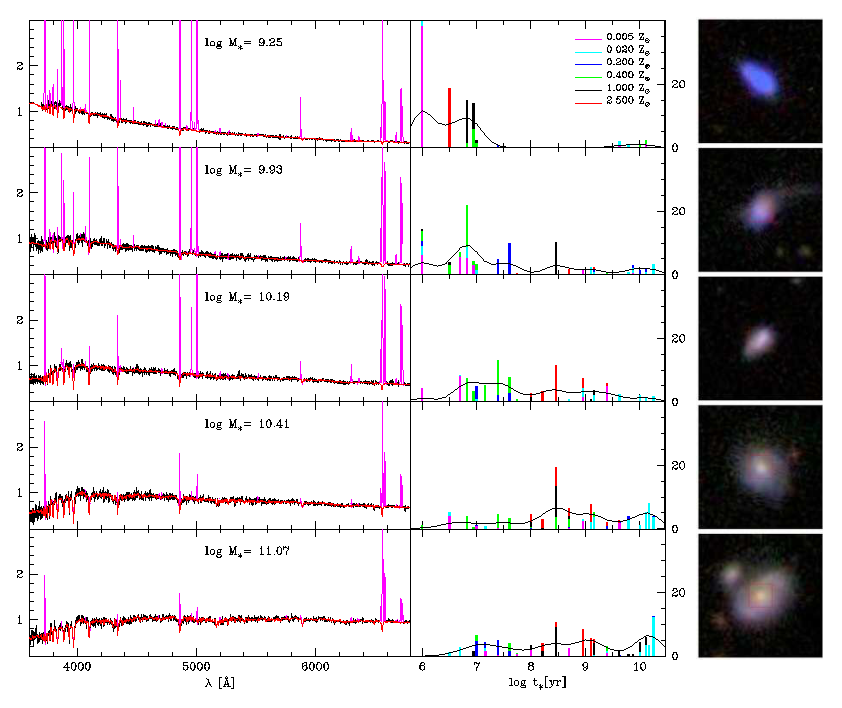
\includegraphics[width=1.0\textwidth]{figuras/starlight-fit}
	\caption[Exemplos de ajuste de espectro com o \starlight]
	{Exemplos de ajuste de espectros de galáxias com o \starlight
	\citep{Asari2007}. À esquerda, espectros observados (preto), espectros
	modelados (vermelho), com regiões mascaradas em magenta. No meio, a fração da
	luz associada a cada uma das 25 idades das SSPs usadas na síntese, com a curva
	representando a versão suavizada do histórico de formação estelar. À direita,
	imagens do SDSS correspondentes às galáxias.}
	\label{fig:StarlightSpectrumSample}
\end{figure}

% FIXME: Rogério - Figura manjada, tu não tens umas tuas?

A aplicação mais imediata do resultado do \starlight é a remoção do contínuo
estelar para medir com maior precisão as linhas de emissão provenientes do gás,
não incluídas no modelo. É possível também estudar o vetor de população
$\vec{x}$, que representa a fração de luz proveniente de cada população estelar
da base (como na coluna central de painéis da Figura
\ref{fig:StarlightSpectrumSample}). De forma alternativa, pode-se utilizar o
vetor de fração de massa $\vec{\mu}$, que se relaciona ao $\vec{x}$ através da
relação massa--luminosidade de cada elemento da base. Individualmente os
componentes $x_j$ e $\mu_j$ dos vetores não são confiáveis, pois há muita
degenerescência nos elementos da base \citep{CidFernandes2005}. Porém, a
informação contida nos vetores pode ser condensada, gerando medidas físicas mais
robustas. A idade estelar média ponderada pela luminosidade pode ser definida
como $\langle \log t \rangle_{\mathrm{L}} = \sum_j x_j \log t_j$, onde $t_j$ é a
idade de cada elemento da base.
Pode-se substituir o vetor de população ($\vec{x}$) pelo vetor de fração de
massa ($\vec{\mu}$) e assim obter a idade ponderada pela massa. Outra
propriedade bastante utilizada é a metalicidade estelar média ponderada pela
massa, definida como $\langle Z \rangle_{\mathrm{M}} = \sum_j \mu_j Z_j$, onde
$Z_j$ é a metalicidade de cada elemento da base. Medidas como estas geram
resultados muito mais confiáveis, como demonstrado por \citet{CidFernandes2014},
reproduzido no Apêndice \ref{apendice:PaperResolving1}.

Esta técnica foi utilizada em diversos artigos. Em particular a colaboração
SEAGal ({\em Semi Empirical Analysis of Galaxies}), liderada pela UFSC, aplicou
o \starlight a 926246 espectros de galáxias do DR7 do SDSS. As propriedades
físicas derivadas desta análise de populações estelares, junto com as medidas de
linhas de emissão, foram disponibilizadas como um banco de dados no {\em
website} \url{http://www.starlight.ufsc.br/}.

Os resultados foram utilizados em estudos varrendo desde a história de formação
estelar de galáxias \citep{Asari2007} a efeitos ambientais \citep{Mateus2007} e
a origem de linhas de emissão de galáxias ``aposentadas'' \citep{Stasinska2008,
CidFernandes2011}. Além desses, pesquisadores em todo o mundo produziram artigos
independentes \citep[para citar alguns]{Bian2006, Liang2007, Peeples2009,
Lara-Lopez2009, Lara-Lopez2010} baseados nesse banco de dados.

Em todos esses estudos, cada galáxia é representada por apenas um espectro. A
extensão desse tipo de estudo a dados IFS parece trivial, e em certa medida o é
se considerarmos o espectro de cada zona (ou {\em spaxel}) como o espectro de
uma galáxia inteira. No entanto, para tirar máximo proveito da informação sobre
populações estelares e sua distribuição espacial é necessária uma ferramenta que
organize os resultados do \starlight para um dado cubo de dados. Dessa
necessidade nasceu a plataforma \pycasso, assunto do próximo capítulo.

% FIXME: Rogério - Sugestões:
%
% * Separar em dois capítulos.
% * Falar um pouco do histórico de aplicaação do starlight (no RS e em SP tem
% trabalhos com isso).

% End of this chapter



  % PyCASSO
  %%%%%%%%%%%%%%%%%%%%%%%%%%%%%%%%%%%%%%%%%%%%%%%%%%%%%%%%%%%%%%%%%
% Tese de Doutorado / Dept Fisica, CFM, UFSC                    %
% Andre@UFSC - 2014                                             %
%%%%%%%%%%%%%%%%%%%%%%%%%%%%%%%%%%%%%%%%%%%%%%%%%%%%%%%%%%%%%%%%%

%:::::::::::::::::::::::::::::::::::::::::::::::::::::::::::::::%
%                                                               %
%                          Capítulo 3                           %
%                                                               %
%:::::::::::::::::::::::::::::::::::::::::::::::::::::::::::::::%

%***************************************************************%
%                                                               %
%                            PyCASSO                            %
%                                                               %
%***************************************************************%

\chapter{PyCASSO}
\label{sec:pycasso}

A fim de agilizar o desenvolvimento de ferramentas de manipulação de cubos de
dados do CALIFA. Este ``kit de ferramentas'' foi chamado de PyCASSO (Python
CALIFA \starlight Synthesis Organizer). PyCASSO foi desenvolvido em Pyton e é, a
grosso modo, composto de três partes.

Conversor de tabelas. Com ele se pode converter a saída do \starlight (arquivos
ASCII para cada pixel de cada galáxia) para cubos de dados nos formatos FITS e
HDF5, de forma a otimizar o acesso aos dados. Uma galáxia leva tipicamente 2
minutos para ser carregada em memória usando arquivos texto. Este tempo se reduz
para menos de um segundo usando arquivo FITS. Há outra otimização para acessar
dados de várias galáxias simultaneamente, utilizando o formato HDF5. Neste caso
a carga dos dados em disco para a memória é ``preguiçosa'', quer dizer, é feita
somente quando os dados são efetivamente acessados.

Camada de entrada e saída. Os arquivos FITS e HDF5 foram montados de forma a
serem facilmente acessados em qualquer ambiente. Ainda assim, há uma camada de
abstração de armazenamento, onde as várias matrizes e cubos são acessadas com
nomes próprios (por exemplo, \texttt{popx},que designa a fração de luz
distribuída pelas populações estelares), de forma a ser possível programar
ferramentas de análise sem precisar se preocupar com as características de cada
formato de armazenamento.

Camada de análise. Como foi mencionado na Seção \ref{sec:Intro:Sintese}, o
resultado da síntese consiste em cubos indexados por zona. Os dados ficam
armazenados no disco desta forma. Porém, na grande maioria das vezes se está
interessado na informação espacialmente resolvida. Esta camada implementa uma rotina de
conversão da notação de zonas para $(x, y)$. Boa parte das propriedades da
síntese, como luminosidade, massa, atenuação por poeira, e idade estelar, já
estão implementadas. Estes cubos espacialmente resolvidos são calculados
dinamicamente, quer dizer, não ocupam memória do sistema até que sejam
acessados. Existem outras rotinas para calcular geometria, perfis radiais e
azimutais, e raio de escala. Outras rotinas podem ser adicionadas
facilmente\footnote{Há um estudo de PCA (análise de componentes principais)
sendo desenvolvido por outro estudante na UFSC, por exemplo.}.

Este software está sendo utilizado pelo grupo de populações estelares da
colaboração do CALIFA, do qual o autor faz parte. No total são aproximadamente
10 pessoas utilizando este software. Foram publicados 4 artigos que utilizam
extensivamente PyCASSO, e mais algun que sutilizaram algum dado resultante de
forma indireta, apresentados na Seção \ref{sec:pycasso:art}.


%***************************************************************%
%                                                               %
%                     PyCASSO - Ferramenta                      %
%                                                               %
%***************************************************************%

\section{A ferramenta de manipulação de cubos de dados PyCASSO}
\label{sec:pycasso:Pycasso}

PyCASSO é uma biblioteca desenvolvida em Python. Porém uma biblioteca não é nada
sem uma boa documentação. Aqui se apresenta de forma breve das capacidades do
PyCASSO. A documentação completa se encontra no Apêndice \ref{apendice:manual}.

O trabalho com a variedade e quantidade de dados gerados pela síntese espectral
de IFS tem em geral um caráter fortemente exploratório. Frequentemente não se
sabe exatamente o que se está buscando, e o trabalho do programador/cientista
consiste em desenhar gráficos, realizar cálculos, determinar operações ou
filtros nos dados com base nestes gráficos e cálculos, desenhar novamente, e
assim sucessivamente. Assim se escolheu a linguagem Python, que possui
ferramentas adequadas à programação exploratória\footnote{Além de estar se
tornando uma espécie de {\em lingua franca} na Astrofísica computacional.}, como
o \texttt{IPython}\footnote{\url{http://ipython.org/}} e o
\texttt{matplotlib}\footnote{\url{http://matplotlib.org/}}. Foi feito um esforço
para que o acesso aos dados de cada galáxia fosse feito de forma simples e
direta, um exemplo de código pode ser visto na Figura \ref{fig:dataAccess}.

\begin{figure}
\begin{python}
# Carregar arquivo FITS com os dados.
from pycasso import fitsQ3DataCube
K = fitsQ3DataCube('K0001_synthesis_suffix.fits')

# Acessar a idade media ponderada pela luminosidade.
at = K.at_flux__z

# Calcular a idade media da galaxia.
at_total = (at * K.Lobn__z).sum() / K.Lobn__z.sum()
print 'Idade media da galaxia: %.2f' % at_total
\end{python}
	\caption[Exemplo de programa utilizando PyCASSO]
	{Exemplo de acesso aos dados. Todas as propriedades estão disponíveis
	diretamente pelo nome, inclusive utilizando a função auto-completar da maioria
	dos ambientes de desenvolvimento Python.}
	\label{fig:dataAccess}
\end{figure}

Para algumas operações, como o cálculo da idade estelar média feito na Figura
\ref{fig:dataAccess}, pode-se utilizar apenas o resultado para as zonas. Neste
caso, a idade estelar média é calculada usando a expressão $\langle \log t
\rangle^{gal}_L = \sum_z \langle \log t \rangle_{L,z} L_z / \sum_z L_z$, onde
$L_z$ é a luminosidade de cada zona e $\langle \log t \rangle_{L,z}$ é a idade
estelar média de cada zona. Entretanto, para tirar vantagem das informações
espaciais, é preciso converter as propriedades da notação de zona para imagem.
Por exemplo, o programa na Figura \ref{fig:programaMapaIdade} calcula a idade
estelar média espacialmente resolvida\footnote{O mapa de idade já está
previamente calculado, disponível através da propriedade
\texttt{at\_flux\_\_yx}. Esta conversão é feita explicitamente aqui para
ilustrar como a conversão pode ser feita para qualquer propriedade.}, e em
seguida desenha um gráfico da imagem gerada (Figura \ref{fig:mapaIdade}).

\begin{figure}
\begin{python}
# Carregar arquivo FITS com os dados.
from pycasso import fitsQ3DataCube
K = fitsQ3DataCube('K0001_synthesis_suffix.fits')

# Converter zonas para imagem.
at_image = K.zoneToYX(K.at_flux__z, extensive=False)

# Desenhar o mapa.
import matplotlib.pyplot as plt
plt.imshow(at_image)
plt.colorbar()
\end{python}
	\caption[Programa para desenhar o mapa da idade estelar média] {Programa
	para desenhar o mapa de idade estelar média ponderada pela luminosidade.}
	\label{fig:programaMapaIdade}
\end{figure}

\begin{figure}
	\includegraphics{figuras/mapa-idade}
	\caption[Mapa da idade estelar média da galáxia IC 5376] {Mapa de idade estelar
	média ponderada pela luminosidade da galáxia IC 5376, desenhado pelo programa
	da Figura \ref{fig:programaMapaIdade}.}
	\label{fig:mapaIdade}
\end{figure}

Enquanto um mapa é uma forma muito boa de visualizar informações em duas
dimensões, há vezes em que uma visualização resumida é mais adequada. Galáxias
em geral têm simetria aproximadamente axial, logo poder medir perfil radial das
propriedades das galáxias é fundamental para estudá-las. Com PyCASSO, o cálculo
do perfil radial é bastante simples, como pode ser visto no programa na Figura
\ref{fig:programaRadprofIdade}, que calcula o perfil radial da idade estelar
média. O resultado está na Figura \ref{fig:radprofIdade}.

\begin{figure}
\begin{python}
# Carregar arquivo FITS com os dados.
from pycasso import fitsQ3DataCube
K = fitsQ3DataCube('K0001_synthesis_suffix.fits')

# Converter zonas para imagem.
at_image = K.zoneToYX(K.at_flux__z, extensive=False)

# Calcular o perfil radial.
bins = np.arange(0, 26, 1)
bin_center = (bins[1:] + bins[:-1]) / 2.0
at_rad = K.radialProfile(at_image, bins, rad_scale=1.0)

# Desenhar o perfil radial.
import matplotlib.pyplot as plt
plt.plot(bin_center, at_rad)
\end{python}
	\caption[Programa para desenhar o perfil radial da idade estelar] {Programa
	para desenhar o perfil radial da idade estelar média ponderada pela
	luminosidade.}
	\label{fig:programaRadprofIdade}
\end{figure}

\begin{figure}
	\includegraphics{figuras/radprof-idade}
	\caption[Perfil radial da idade estelar média da galáxia IC 5376] {Perfil
	radial da idade estelar média ponderada pela luminosidade da galáxia IC
	5376, desenhado pelo programa da Figura \ref{fig:programaRadprofIdade}.}
	\label{fig:radprofIdade}
\end{figure}

Esta é só uma pequena demonstração das ferramentas existentes no PyCASSO. Também
é possível trabalhar com espectros, calcular perfis azimutais, lidar com pixels
mascarados, entre outras coisas. Tudo isto está descrito em detalhes no manual
do programa (Apêndice \ref{apendice:manual}).


%***************************************************************%
%                                                               %
%                      PyCASSO - Artigos                        %
%                                                               %
%***************************************************************%

\section{Artigos publicados}
\label{sec:pycasso:art}

Nesta seção discute-se os artigos onde se utilizou PyCASSO, e o autor desta tese
teve uma colaboração importante. Além destes artigos, \citet{Husemann2013}, no
artigo apresentando o DR1 do CALIFA, utiliza as massas estelares determinadas
pelo \starlight e disponibilizadas pelo PyCASSO para caracterizar a amostra do
CALIFA.
O artigo que apresenta o DR2, de \citet{GarciaBenito2015}, também utiliza as
massas da mesma forma (ver Figura \ref{fig:DRMass}). O mesmo artigo inclui a
medição da PSF do CALIFA (ver Figura \ref{fig:DR2PSF}), apresentado neste
trabalho na Seção \ref{sec:psf:medida}. Em \citep{GonzalezDelgado2015} se
utiliza, além de PyCASSO, a decoposição bojo--disco (ver Seção
\ref{sec:morph:comp:bd}) em uma amostra de galáxias, realizada pelo autor desta
tese, adaptando técnicas discutidas no Capítulo \ref{sec:Decomp}.

\TODO Letter da Rosa? \citet{IglesiasParamo2013}?


%***************************************************************%
%                                                               %
%       PyCASSO - Resolving galaxies in Space and Time I        %
%                                                               %
%***************************************************************%

\subsection{Artigo: {\em Resolving galaxies in time and space. I. Applying
STARLIGHT to CALIFA datacubes}}
\label{sec:pycasso:art:Resolving1}

Este artigo por \citet{CidFernandes2013} descreve todo o processo de síntese
espectral dos cubos de dados do CALIFA, mencionados no Capítulo \ref{sec:intro},
e serve como uma demonstração da capacidade do PyCASSO. O artigo está
reproduzido na íntegra no Apêndice \ref{apendice:PaperResolving1}. O
preprocessamento dos cubos de espectros é feito através do programa QBICK,
desenvolvido por Rubén Garcia Benito especialmente para o CALIFA, mas é genérico
o bastante para ser usado em outros cubos de dados. Após explicar em detalhes
todos os passos envolvidos desde o preprocessamento, passando pela descrição do
\starlight até a importação dos dados pelo PyCASSO, o artigo apresenta um caso
de estudo com a galáxia NGC 2916.

\begin{figure}
	\includegraphics{figuras/L-M-AV-K0277}
	\caption[Propriedades físicas espacialmente resolvidas para a galáxia NGC
	2916] {Propriedades físicas espacialmente resolvidas para a galáxia NGC 2916. (a)
	Luminosidade em $5635\,\angstrom$ por unidade de área. (b) Atenuação por
	poeira na banda $V$. (c) Luminosidade em $5635\,\angstrom$ por unidade de área,
	corrigido de extinção. (d) Desidade superficial de massa estelar. Retirado de
	\cite[figura 4]{CidFernandes2013}, Apêndice \ref{apendice:PaperResolving1}.}
	\label{fig:LMAVMap}
\end{figure}


\begin{figure}
	\includegraphics{figuras/at-aZ-K0277}
	\caption[Idade estelar e metalidade espacialmente resolvidas para a
	galáxia NGC 2916] {Idade e metalicidade estelar média, espacialmente
	resolvidas, para a galáxia NGC 2916. (a) Idade estelar média pesada pela
	luminosidade. (b) metalicidade estelar média pesada pela luminosidade.
	(c) Idade estelar média pesada pela massa. (d) metalicidade estelar
	média pesada pela massa. Retirado de
	\cite[figura 6]{CidFernandes2013}, Apêndice \ref{apendice:PaperResolving1}.}
	\label{fig:ataZMap}
\end{figure}

% TODO: corrigir largura
\begin{figure}
	\includegraphics[width=1.0\columnwidth]{figuras/L-M-SFR-K0277}
	\caption[Diagramas $R \times t$ para luz, massa e SFR] {Diagramas $R \times t$
	para luz, massa e taxa de formação estelar (SFR). (a) Luminosidade em
	$5635\,\angstrom$ por unidade de área.  (b) Massa transformada em estrelas por
	unidade de área. (c) Taxa de formação estelar por unidade de área. A linha
	sólida representa o gráfico colapsado na direção vertical, apenas para ilustrar
	a variação temporal das quantidades mapeadas. Retirado de
	\cite[figura 12]{CidFernandes2013}, Apêndice \ref{apendice:PaperResolving1}.}
	\label{fig:LMSFR2D}
\end{figure}

As Figuras \ref{fig:LMAVMap} e \ref{fig:ataZMap} mostram mapas de propriedades
físicas obtidas pela síntese espectral. Propriedades como a massa (Figura
\ref{fig:LMAVMap}d) e luminosidade (Figuras \ref{fig:LMAVMap}a e
\ref{fig:LMAVMap}c) são quantidades extensivas, e são proporcionais à escala. Já
a atenuação por poeira (Figura \ref{fig:LMAVMap}b), idade e metalicidade estelar
são quantidades intensivas, independentes de escala. Na prática isto significa
que as quantidades extensivas podem ser divididas entre os pixels que compõem
uma zona, enquanto as intensivas são uma propriedade comum à todos os pixels
desta zona. Esta diferença pode ser notada nas zonas mais externas dos mapas,
onde aparecem platôs na quantidades intensivas. As quantidades extensivas passam
por um processo apelidado de ``dezonificação''\fixme, descrito na Seção
\ref{sec:pycasso:Pycasso}.

Um dos desafios de se trabalhar com cubos multidimensionais é como visualizar
esta informação. Uma alternativa é comprimir determinadas dimensões. Para
ilustrar esta capacidade do PyCASSO, a Figura \ref{fig:LMSFR2D} mostra diagramas
de luz, massa e taxa de formação estelar (SFR) em função do tempo, onde as
dimensões $x$ e $y$ foram transformadas em distância radial. Diagramas como
este, junto com perfis 1-D radiais e temporais ajudam a visualizar e interpretar
o resultado da síntese espectral, oferecendo novas ferramentas para estudar a
estrutura e evolução de galáxias.


%***************************************************************%
%                                                               %
%       PyCASSO - Resolving galaxies in Space and Time II       %
%                                                               %
%***************************************************************%

\subsection{Artigo: {\em Resolving galaxies in time and space: II: Uncertainties
in the spectral synthesis of datacubes}}
\label{sec:pycasso:art:Resolving2}

Uma crítica bastante comum aos métodos de ajuste é que eles não provêm a
incerteza associada aos valores ajustados. A forma mais simples de determinar
esta incerteza é refazer o ajuste várias vezes, perturbando as medidas
reproduzindo de forma realista os erros. Este artigo por
\citet{CidFernandes2014} investiga a incerteza nos ajustes feitos no artigo
discutido na seção anterior. O artigo está reproduzido na íntegra no Apêndice
\ref{apendice:PaperResolving2}.

Quando se injeta erros aleatórios, obtém-se incertezas de $\sim
0.08\,\mathrm{dex}$ em idades e metalicidades pesadas pela luminosidade, e de
$\sim 0.15\,\mathrm{dex}$ quando pesadas pela massa. A massa estelar teve uma
incerteza de $\sim 0.08\,\mathrm{dex}$, e $A_V$ de $\sim 0.06\,\mathrm{mag}$.
Injetando erros sistemáticos em cor\footnote{Adicionando componentes lineares em
comprimento de onda, a fim de emular uma má calibração de fluxo.} os erros são
similares, exceto para $A_V$, que recebe um desvio sistemático de
$+0.05\,\mathrm{mag}$ e um erro de $\sim 0.16\,\mathrm{mag}$.

\begin{figure}
	\includegraphics[width=1.0\columnwidth]{figuras/resolving2}
	\caption[Incerteza nos perfis radiais] {Incerteza nos perfis radiais de
	algumas propriedades. (a) Luminosidade superficial a $5635\,\angstrom$,
	corrigida de extinção. (b) Densidade superficial de massa. (c) Atenuação na
	banda $V$. (d) Taxa de formação estelar (últimos $140\, \mathrm{Ma}$) por
	unidade de área. (e) Idade estelar média ponderada pela luminosidade. (f) Idade
	estelar média ponderada pela massa. (g) Metalicidade estelar média ponderada
	pela luminosidade. (h) Metalicidade estelar média ponderada pela massa. As
	linhas em preto marcam a solução original. Em faixas azuis e vermelhas, as
	distribuições das realizações com ruído aleatório, e sistemático em cor,
	respectivamente. A diferença entre as simulações e o original está desenhada
	abaixo de cada painel, com o zero marcado pela linha tracejada. Retirado de
	\cite[figura 4]{CidFernandes2014}, Apêndice \ref{apendice:PaperResolving2}.}
	\label{fig:incertRad}
\end{figure}

Embora haja uma incerteza considerável analisando-se as propriedades da galáxia
pixel a pixel, os perfis radiais em geral são bastante robustos. Propriedades
diretas como a luminosidade, massa, idade e metalicidade estelar, quando vistas
em perfil radial (Figura \ref{fig:incertRad}) mantém o mesmo formato com pouca
dispersão, exceto nas regiões mais afastadas do núcleo, onde há poucas zonas. Na
verdade, qualquer forma de média espacial que envolva pixels (ou zonas)
suficientes deverá levar a uma diminuição na incerteza.

% FIXME: corrigir largura da figura
\begin{figure}
	\includegraphics[width=1.0\columnwidth]{figuras/resolving2-base}
	\caption[Comparação dos ajustes com bases de SSP diferentes]
	{Comparação de propriedades obtidas com o ajuste utilizando as bases
	GM (eixo vertical) CB (eixo horizontal). Os painéis superiores mostram um
	histograma 2-D com contornos para propriedades de cada pixel de 107 galáxias do
	CALIFA. Da esquerda para a direita: idade estelar ponderada pela luminosidade,
	metalicidade estelar ponderada pela massa, atenuação na banda $V$, massa
	estelar inicial. Os painéis inferiores mostram a distribuição das mesmas
	propriedades, porém calculadas para o espectro integradas das galáxias.
	Retirado de \cite[figura 9]{CidFernandes2014}, Apêndice
	\ref{apendice:PaperResolving2}.}
	\label{fig:incertRad-base}
\end{figure}

O artigo também explora os efeitos da escolha da base de SSPs nos resultados do
ajuste. Em geral, bases diferentes levam a resultados consistentes.
Pode-se ver na Figura \ref{fig:incertRad-base} que a idade estelar
média ponderada pela luminosidade, a atenuação e a massa estelar inicial
têm uma concordância muito boa entre as bases. As metalicidades médias mostram
uma correlação, mas com uma dispersão muito grande, certamente devido a
diferenças nas trajetórias evolucionárias dos modelos, poucos valores
de metalicidade na base, e diferenças na metalicidade máxima da base. A
incerteza nestas propriedades mencionadas acima é cerca de $2$ vezes maior do
que as calculadas adicionando ruído aleatório. Claramente a escolha de uma base
adequada é de grande importância para a análise.


%***************************************************************%
%                                                               %
%                 PyCASSO - Inside-out growth                   %
%                                                               %
%***************************************************************%

\subsection{Artigo: {\em The Evolution of Galaxies Resolved in Space and Time: A
View of Inside-out Growth from the CALIFA Survey}}
\label{sec:pycasso:art:InsideOut}

Em \citet{Perez2013} se estuda o crescimento de dentro para fora de $105$
galáxias do CALIFA. O estudo se baseia na síntese espectral com o \starlight, e
segue exatamente a mesma prescrição de \citet{CidFernandes2014}, descrita na
Seção \ref{sec:pycasso:art:Resolving1}. O artigo está reproduzido na íntegra no
Apêndice \ref{apendice:InsideOut}.

Galáxias vêm em todos os tamanhos. Para determinar o crescimento, as distâncias
são normalizadas em utilizando o raio onde a luminosidade cumulativa (em
$5635\,\angstrom$) alcança $50\%$ da luminosidade total da galáxia, denominado
$R_{50}$. As galáxias da amostra são separadas em {\em bins} com $15$ galáxias
cada, segundo a sua massa. O crescimento em massa em função do tempo é calculado
para cada pixel de cada galáxia e somado em cada {\em bin} de massa.

\begin{figure}
	\includegraphics{figuras/inside-out}
	\caption[Crescimento da massa estelar de galáxias de dentro para fora]
	{Crescimento de massa estelar de dentro para fora. As $105$ galáxias foram
	separadas em grupos de 15, em massa, formando os {\em bins} do eixo vertical.
	Os painéis mostram o crescimento da massa em escala de cinza, normalizado, em
	função do tempo e da massa das galáxias. O contorno em preto marca $80\%$. Da
	direita para a esquerda se vê as regiões em raio $r < 0,1\,R_{50}$, $0,1 < r
	\leq 0,5\,R_{50}$, $0,5 < r \leq 1\,R_{50}$ e $r > 1\,R_{50}$. Para
	facilitar a visualização da forma da variação temporal, as linhas azuis, verdes
	e vermelhas em cada painel mostram um corte horizontal nos {\em bins} inferior,
	intermediário e superior, com escala de $0$ a $1$. Retirado de \cite[figura
	9]{Perez2013}, Apêndice \ref{apendice:InsideOut}.}
	\label{fig:insideOut}
\end{figure}

A Figura \ref{fig:insideOut} ilustra o crescimento de massa em anéis crescentes
em raio ($0,1\,R_{50}$, $0,5\,R_{50}$, $1\,R_{50}$ e $>1\,R_{50}$.). Em cada
painel, o tempo passa da direita para a esquerda, e a massa estelar,
normalizada, cresce desde zero (direita, em preto) até $1$ (esquerda, em
branco). Se vê claramente que galáxias menos massivas, na parte inferior dos
{\em bins}, têm um crescimento gradual mais ou menos constante em todos os
raios. As galáxias mais massivas, a parte superior dos {\em bins}, apresentam um
crescimento muito rápido nas regiões centrais, enquanto as regiões externas
crescem mais gradualmente. As linhas azul, verde e vermelha, em cada painel,
representam cortes horizontais no {\em bin} de mais baixa massa, no
intermediário e no de mais alta massa, respectivamente, para facilitar a
visualização. A mudança de regime ocorre em $\log M\star = 10,83$, ou seja, uma
massa de $\sim 7\times10^{10}\,M_\odot$. O autor cita vários estudos que indicam
esta faixa como uma ``massa especial'', onde a taxa de formação estelar alcança
valores altos muito rapidamente. De qualquer forma, esta é uma evidência
observacional de algo que já se suspeita há muito tempo:
que as galáxias massivas se formaram de dentro para fora.


%***************************************************************%
%                                                               %
%                 PyCASSO - Radial structures                   %
%                                                               %
%***************************************************************%

\subsection{Artigo: {\em The star formation history of CALIFA galaxies: Radial
structures}}
\label{sec:pycasso:art:RadStruct}

O artigo por \citet{GonzalezDelgado2014a} faz um estudo detalhado da estrutura
radial de diversas propriedades de $107$ galáxias do CALIFA. O artigo está
reproduzido na íntegra no Apêndice \ref{apendice:RadStruct}.
Um dos resultados mais importantes é que a densidade superficial de massa
estelar e idade estelar média ponderada por luminosidade, medidas a $1\,R_{50}$,
são representativos das médias da galáxia como um todo. A Figura
\ref{fig:radStruct1} mostra a correlação entre os valores em três raios
distintos e o global para a idade estelar média ponderada pela luminosidade
(esquerda) e a densidade superficial de massa estelar (centro). Valores a
$1\,R_{50}$, marcado como HLR ({\em Half Light Radius}) nas figuras, coincidem
em geral com a média global da galáxia.
Ainda na mesma figura pode-se ver a correlação entre a densidade superficial de
massa estelar média da galáxia e a massa estelar total da galáxia. Este
resultado está de acordo com \citet{Kauffmann2003}, usando a amostra do SDSS.

\begin{figure}
	\includegraphics[width=1.0\columnwidth]{figuras/radstruct-01}
	\caption[Correlação entre idade, desidade superficial e massa estelar total]
	{(esquerda) Correlação entre a idade estelar média ponderada pela luminosidade
	em $1\,R_{50}$ (círculos cinza), $0,1\,R_{50}$ (cruzes azuis), $2\,R_{50}$
	(cruzes vermelhas) e a média da galáxia. Pontos em preto marcam galáxias
	esferoidais, com $C \geq 2,8$. (centro) O mesmo gráfico para a densidade
	superficial de massa estelar. (direita) Correlação entre a densidade
	superficial de massa média da galáxia e a massa estelar total da galáxia. As
	linhas tracejadas mostram o ajuste linear total (preto), apenas discos (azul),
	e apenas para esferoidais (vermelho).  Retirado de \cite[figura
	6]{GonzalezDelgado2014a}, Apêndice \ref{apendice:RadStruct}.}
	\label{fig:radStruct1}
\end{figure}

O raio contendo metade da massa estelar (HMR, {\em Half Mass Radius}) é em média
20\% menor que $R_{50}$ (HLR). A razão entre HMR e HLR tem correlação com a
massa total da galáxia e o tipo morfológico. Na Figura \ref{fig:radStruct2}
pode-se ver que a relação HMR/HLR diminui com a massa estelar para galáxias com
massa menor que $10^{11}\,M_\odot$, enquanto permanece constante para galáxias
mais massivas. Um comportamento similar ocorre com o tipo morfológico:
em galáxias com disco a relação HMR/HLR diminui com a massa, e em galáxias
esferoidais a relação é aproximadamente constante.

\begin{figure}
	\includegraphics{figuras/radstruct-02}
	\caption[Relação entre $a^M_{50}/a^L_{50}$ e a massa estelar total]
	{Relação entre $a^M_{50}/a^L_{50}$ e a massa estelar total. A cor dos
	pontos reflete a idade estelar média ponderada pela luminosidade, em $0,5\,a^L_{50}$.
	Galáxias com índice de concentração $C \geq 2,8$ estão marcadas com uma cruz. A
	linha azul mostra o ajuste linear para galáxias com massa estelar Retirado de
	\cite[figura 10]{GonzalezDelgado2014a}, Apêndice
	\ref{apendice:RadStruct}.}
	\label{fig:radStruct2}
\end{figure}

Para galáxias esferoidais, o gradiente de idade depende mais da massa estelar
total da galáxia do que da densidade superficial de massa estelar, que, conforme
o painel inferior esquerdo da Figura \ref{fig:radStruct3}, é aproximadamente
constante. A massa total da galáxia é a propriedade mais fundamental para
galáxias esferoidais, enquanto a densidade superficial de massa é mais
importante para as galáxias com disco.


\begin{figure}
	\includegraphics[width=0.8\columnwidth]{figuras/radstruct-03}
	\caption[Perfis radiais para vários {\em bins} de massa estelar.]
	{Perfis radiais da densidade superficial de massa estelar (esquerda) e idade
	estelar média ponderada pela luminosidade (direita), para {\em bins} de
	massa estelar contendo 15 galáxias cada. (cima) Todas as galáxias. Os {\em
	bins} em massa estão codificados em cores. (meio) Galáxias dominadas por
	disco. (baixo) Galáxias esferoidais ($C \geq 2,8$). Retirado de \cite[figura
	13]{GonzalezDelgado2014a}, Apêndice \ref{apendice:RadStruct}.}
	\label{fig:radStruct3}
\end{figure}


% End of this chapter

  
  % Morfologia de galáxias
  %%%%%%%%%%%%%%%%%%%%%%%%%%%%%%%%%%%%%%%%%%%%%%%%%%%%%%%%%%%%%%%%%
% Tese de Doutorado / Dept Fisica, CFM, UFSC                    %
% Andre@UFSC - 2014                                             %
%%%%%%%%%%%%%%%%%%%%%%%%%%%%%%%%%%%%%%%%%%%%%%%%%%%%%%%%%%%%%%%%%

%:::::::::::::::::::::::::::::::::::::::::::::::::::::::::::::::%
%                                                               %
%                          Capítulo 4                           %
%                                                               %
%:::::::::::::::::::::::::::::::::::::::::::::::::::::::::::::::%

%***************************************************************%
%                                                               %
%                   Morfologia de galáxias                      %
%                                                               %
%***************************************************************%

\chapter{Morfologia de galáxias}
\label{sec:morph}

A descoberta das formas das galáxias, e a sua separação em classes segundo a sua
morfologia, somente se tornou uma ciência séria quando {\em surveys}
fotográficos extensos começaram a ser realizados \citep{Sandage1975}. Pode-se
considerar o ano de 1845 como um marco inicial no estudo da forma das galáxias,
quando Lord Rosse, observando com o telescópio refletor de 72 polegadas no
Castelo de Burr, descobriu estruturas espirais em M51 (Galáxia do Redemoinho, no
catálogo de Messier). À época, pouco se sabia sobre a natureza das ``nebulosas
espirais'' e os esquemas de classificação eram puramente descritivos como o de
\citet{Wolf1908}, mostrado na Figura \ref{fig:WolfEarlyClass}.
\citet{Knox-Shaw1915}, entre outros, chamou a atenção para nebulosas sem braços
espirais, que viriam a ser chamadas mais tarde de elípticas.
\citet{Curtis1918} foi o primeiro a identificar espirais com barra.
Em meados de 1940 já se havia descoberto a maioria dos tipos mais comuns das
``nebulosas extragaláticas'', termo que já começava a cair em desuso em favor do
nome mais glamouroso, segundo o próprio \citet{hubble1936}: ``galáxias''.

\begin{figure}
	\includegraphics[width=0.7\textwidth]{figuras/WolfEarlyClass}
	\caption[Classificação de Wolf.]
	{Sistema de classificação descritivo de nebulosas por \citet{Wolf1908},
	apresentava também nebulosas galáticas (na primeira linha, que foi removida).
	Reproduzido de \citet{Sandage1975}.}
	\label{fig:WolfEarlyClass}
\end{figure}


%***************************************************************%
%                                                               %
%                   Classificação de Hubble                     %
%                                                               %
%***************************************************************%

\section{Classificação de Hubble}

O primeiro sistema amplamente utilizado de classificação de galáxias segundo a
sua morfologia foi o de \citet{Hubble1926}. Neste sistema, as galáxias são
separadas nas classes elíptica, espiral, espiral com barra e irregular. As
elípticas são classificadas segundo o seu formato, desde esférico até mais
alongado. As espirais são classificadas conforme o tamanho relativo do bojo e as
características dos braços (quantidade, grau de espiralamento e granularidade).
A forma final de classificação de Hubble é frequentemente ilustrada pelo
``diagrama diapasão'', apresentado na Figura \ref{fig:HubbleSequence}, do
clássico {\em The Realm of the Nebulae} de \citet{hubble1936}, e atualizado
(incluindo o tipo S0 na intersecção dos ramos das espirais) por
\citet{Sandage1975}.

\begin{figure}
	\includegraphics[width=1.0\textwidth]{figuras/HubbleSequence}
	\caption[Classificação de Hubble.]
	{Sistema de classificação de \citet{hubble1936}, também conhecido como
	``diagrama diapasão de Hubble''. Foi atualizado por
	\citet{Sandage1975} para incluir o tipo S0 na intersecção dos
	ramos das espirais.}
	\label{fig:HubbleSequence}
\end{figure}

O sistema de Hubble parece ser mais do que um simples ``catálogo botânico'' de
galáxias. Muitas das propriedades observadas das galáxias, como índices de cor,
tipo espectral e densidade de hidrogênio gasoso, variam sistematicamente na
sequência de formas\fixme(referêcias!). De algum modo, parece haver algo de
fundamental escondido nesta classificação baseada apenas na forma, que talvez
indique uma relação com as condições iniciais e subsequente evolução temporal
das galáxias \citep{Sandage1975}. Estas correlações fizeram com que, durante
muito tempo, a sequência de Hubble fosse considerada uma sequência evolutiva,
onde as galáxias eram inicialmente elípticas, passavam a ser lenticulares e
depois espirais. Isto sobrevive até hoje na nomenclatura ``tipo jovem'' para
elípticas e lenticulares, e ``tipo tardio'' para espirais e irregulares.
Entretanto, \citet{Hubble1927} enfatizou desde o início que a classificação era
puramente empírica, e que interpretações de natureza evolutiva deveriam ser
tomadas com cautela.


%***************************************************************%
%                                                               %
%                   Componentes estruturais                     %
%                                                               %
%***************************************************************%

\section{Componentes estruturais}

Os sistemas de classificação descritos na seção anterior são baseados em
inspeção visual, com natureza evidentemente qualitativa. Levando tal forma de
classificação a um extremo, como o projeto {\em GalaxyZoo} \citep{Lintott2008,
Willett2013}, chega-se a conclusões estatísticas, mas ainda não se obtém medidas
quantitativas de objetos individuais. Para descrever mais precisamente a
estrutura de uma galáxia, normalmente é necessário decompô-la em sub-estruturas.
Estas sub-estruturas são em geral modeladas como funções analíticas, as quais
permitem derivar medidas quantitativas. De forma simplificada, podemos
considerar que galáxias são compostas de duas componentes principais: bojo e
disco. Os próprios discos podem conter barras, braços espirais, anéis e halos,
para citar algumas sub-componentes mais comuns.


\subsection{Bojos e discos}

Do ponto de vista fotométrico, medindo o perfil de brilho superficial, galáxias
lenticulares (S0) e espirais tipo jovem (Sa-Sb) podem ser bem descritas como uma
combinação de duas componentes: um bojo e um disco. Neste modelo, o disco é
razoavelmente fino, enquanto o bojo é quase esférico (embora haja casos em que
ele seja um elipsóide triaxial), ambos observados projetados no plano do céu.

Levando em consideração apenas o perfil de brilho superficial, esta separação
pode parecer arbitrária. Afinal, pode-se inventar alguma lei empírica onde uma
só componente descreva as imagens observadas tão bem quanto a soma de um bojo e
um disco. Porém, há outras observações que suportam a separação nestas duas
componentes. \TODO Referências! Provavelmente alguma coisa a ver com cinemática
(rotação e dispersão) e populações estelares.

\begin{figure}
	\includegraphics[width=0.5\textwidth]{figuras/test}
	\caption[Leis empíricas de perfil de brilho.]
	{\TODO Leis empíricas de perfil de brilho.}
	\label{fig:MorphLaws}
\end{figure}

\citet{King1966} descreve um modelo derivado para aglomerados globulares,
assumindo velocidades estelares isotérmicos e isotrópicas. Muito embora este
modelo tenha motivações físicas, não possui uma forma funcional simples. Leis
como as de Hubble-Reynolds \citep[equação 2.55]{Binney2011} e
\citet{deVaucouleurs1948, deVaucouleurs1977}, mesmo sendo puramente empíricas,
descrevem bem bojos de galáxias. Suas formas funcionais são:
\begin{equation*}
I(r) &= \frac{I_0}{\left[1 + \left(\sfrac{r}{r_H}\right)^2\right]}
&\text{(Hubble-Reynolds)} \\
I(r) &= I_e \exp \left\{-7,67 \left[\left(\frac{r}{r_e}\right)^2 -
1\right]\right\} &\text{(de Vaucouleurs)}
\end{equation*}

Os termos $r_e$ e $r_H$ são os parâmetros de escala radial, $I_0$ é o
brilho para $r=0$ na lei de Hubble-Reynolds e $I_e$ é o brilho para $r=r_e$ na
lei de de Vaucouleurs. Estas formas funcionais se ajustam bem à maioria dos
bojos e galáxias elípticas. Para sistemas que não são esféricos, deve-se ainda
introduzir uma elipticidade e uma orientação. Adicionalmente, a elipticidade e a
orientação podem variar com o raio.

Discos, por outro lado, são facilmente modelados como um perfil exponencial
\citep{Freeman1970} dado por
\begin{equation*}
I(r) = I_0 \exp\left(\frac{r}{h}\right),
\end{equation*}
com $h$ sendo o parâmetro de escala radial, e $I_0$ o brilho em $r=0$. \TODO
Por que o disco é exponencial? Referências!

\citet{Sersic1963} mostra que os perfis de de Vaucouleurs e exponencial podem
ser tomados como casos particulares da equação
\begin{equation*}
I(r) = I_e \exp \left\{- b_n \left[ \left( \frac{a}{r_e} \right)^{\sfrac{1}{n}}
- 1 \right] \right\},
\end{equation*}
que ficou conhecida como ``lei de Sérsic''. Aqui, o parâmetro $n$ é o índice de
concentração, também chamado de ``índice de Sérsic'', que pode variar
continuamente. Com $n=1$ obtém-se uma lei exponencial, e com $n=4$ a lei de de
Vaucouleurs. A maioria dos bojos e galáxias elípticas podem ter seus perfis
de brilho ajustados com índices de Sérsic na faixa de $1 < n < 10$. O parâmetro
$b_n$ está definido em função de $n$, ver a seção 6.1.5 de \citet{Erwin2015}.

\TODO Caveat emptor: cuidado ao interpretar demais leis empíricas!


\subsection{Dependência dos modelos com o comprimento de onda}
\label{sec:morph:comp:depLambda}

\TODO Mais referências e blablabla antes!

\citet{Kelvin2012} utilizou imagens de galáxias do projeto GAMA
\citep{Driver2009} em 9 bandas espectrais, do óptico \citep[bandas $ugriz$ do
DR7]{Abazajian2009} ao infravermelho \citep[bandas $YJHK$ do
UKIDSS]{Lawrence2007}, para ajustar perfis de Sérsic a $>160\,000$ galáxias,
encontrando gradientes leves no índice de Sérsic em função do comprimento de
onda.

\begin{figure}
	\includegraphics{figuras/vika-properties}
	\caption[Ajuste morfológico de bandas fotométricas] {Ajuste
	morfológico de 11 galáxias, utilizando as bandas fotométricas do
	SDSS. Os gráficos mostram o raio efetivo ($r_e$ neste trabalho) ajustado
	livremente a cada banda (painéis superiores), e com uma dependência linear em
	comprimento de onda (painéis inferiores). À esquerda estão os ajustes com as
	imagens originais, as colunas seguintes são para imagens com {\em redshift}
	artificiais. Retirado de \citet{Vika2013}.}
	\label{fig:propertiesVika}
\end{figure}

\TODO O projeto MegaMorph \citep{Haussler2013} está fazendo o ajuste morfológico
dependente de comprimento de onda de imagens de galáxia. A diferença é que no
caso do MegaMorph utiliza-se imagens de fotometria de banda larga do SDSS, e
eles ajustam a variação dos parâmetros morfológicos através de um polinômio
\citep[Figura \ref{fig:propertiesVika}]{Vika2013}. Aí se pode ver que em grande
escala (em comprimento de onda), há galáxias com um comportamento linear (ou até
razoavelmente constante) em $r_e$, porém outras apresentam variações mais
complexas. Este problema deve ser estudado mais a fundo futuramente neste
trabalho.

\TODO: O que pode causar a variação?

População estelar \citep{LaBarbera2009}.

Poeira em discos \citep{Mollenhoff2006}.

\begin{figure}
	\includegraphics{figuras/johnston-spectra}
	\caption[Espectros das componentes morfológicas] {Espectros unidimensionais de
	disco e bojo de NGC 1375. Retirado de \citet{Johnston2012}.}
	\label{fig:spectraJohnston}
\end{figure}

\citet{Johnston2012} obtiveram um espectro de fenda de galáxias lenticulares
(S0), tendo assim um perfil de brilho da galáxias para cada comprimento de onda.
Ajustando um perfil de Sérsic e um exponencial a cada um dos perfis, eles obtém
os espectros separados de cada um dos componentes morfológicos (Figura
\ref{fig:spectraJohnston}). \TODO Que conclusões chegam?


\subsection{Ajuste de modelos}


Utiliza-se geralmente algoritmos de minimização para encontrar os modelos que
melhor ajustam o perfil de brilho de uma galáxia. A abordagem usual é baseada no
princípio de máxima verossimilhança ($\mathcal{L}$). Se a estatística das
medidas é gaussiana (que é aproximadamente verdade na maioria das imagens
astronômicas relevantes ao ajuste de modelos), o logarítmo da verossimilhança se
assemelha à familiar soma de $\chi^2$\citep[seção 4.1.2]{Erwin2015}. Isto
significa que o problema passa a ser a minimização da equação
\begin{equation*}
-2\ln\mathcal{L} = \chi^2 = \sum_i^N \frac{\left(d_i -
m_i\right)^2}{\sigma_i^2},
\end{equation*}
onde $d_i$ é o valor medido, $m_i$ é o valor do modelo, e $\sigma_i$ é o erro
gaussiano na medida. O modo como se procura o mínimo $\chi^2$ vai depender de
como se aborda o problema.

\begin{figure}
	\includegraphics{figuras/johnston-decomp}
	\caption[Ajuste morfológico em uma dimensão] {Ajuste morfológico
	em uma dimensão, utilizando modelos de bojo e disco. A linha preta mostra o
	perfil de brilho da galáxia NGC 1375 em $5195\,\angstrom$, obtido através de
	espectroscopia de fenda longa. Em azul um perfil exponencial e em vermelho um
	perfil de De Vaucouleurs (Sérsic com $n=4$), que somados são o melhor ajuste,
	em verde. Retirado de \citet{Johnston2012}.}
	\label{fig:decompJohnston}
\end{figure}

\begin{figure}
	\includegraphics[width=0.5\textwidth]{figuras/test}
	\caption[Ajuste morfológico em duas dimensões] {\TODO Ajuste morfológico
	em duas dimensões, utilizando modelos de bojo e disco. Pegar alguma figura do
	GALFIT3 \citep{Peng2010}.}
	\label{fig:decompGalfit}
\end{figure}

A figura \ref{fig:decompJohnston} mostra um exemplo de ajuste de bojo e disco em
um perfil de brilho unidimensional. Pode-se fazer o ajuste diretamente na
imagem, em duas dimensões (Figura \ref{fig:decompGalfit}), utilizando modelos
com perfis elipsoidais. Independente da escolha do modelo, há um aspecto
importante do ajuste da morfologia que foi negligenciado até agora: efeitos
instrumentais e atmosféricos. Estes efeitos são representados pela figura da
PSF, tratados em detalhes no Capítulo \ref{sec:psf}. A grosso modo, levar em
conta a PSF significa considerar que a luz que atinge determinada posição no
detector não é proveniente apenas de uma região pontual no céu, e sim de uma
região extensa que depende dos instrumentos e da tubulência atmosférica.
Efetivamente, objetos pontuais tornam-se ``borrões'' na imagem observada.

Pode-se evitar tocar neste ponto quando se faz o ajuste em uma dimensão.
Se as dimensões da PSF forem muito menores do que as da galáxia, e esta tiver
uma imagem suave, a forma da galáxia muda muito pouco devido à PSF, exceto
exatamente sobre o núcleo. Isto é especialmente problemático em tipos jovens,
onde um perfil de Sérsic pode gerar um pico de várias ordens de magnitude,
concentrado em uns poucos em {\em pixels}. A forma mais simples de se escapar da
PSF, em uma dimensão, é ``varrê-la para baixo do tapete'', isto é, não tentar
ajustar pontos muito próximos ao núcleo (mascarando alguns segundos de arco,
dependendo do tamanho da PSF). O ajuste de um perfil de Sérsic pode ficar
comprometido em casos onde a PSF é muito grande e se descarta uma fração
considerável do bojo.\fixme(Referência!)

Em duas dimensões o mais adequado é adotar a PSF como parte do problema. Uma boa
caracterização da PSF é crucial para se obter resultados satisfatórios no
ajuste. Mas, trabalhar com a PSF traz um custo computacional enorme, agora é
preciso efetuar um cálculo de convolução\footnote{O custo computacional de fazer
convolução da imagem com uma PSF pode ser aliviado utilizando uma transformada
de Fourier, valendo-se da propriedade $\mathcal{F}\left\{f \mathbin{*} g\right\}
= \mathcal{F}\left\{f\right\} \cdot \mathcal{F}\left\{g\right\}$. Ainda assim é
preciso calcular uma transformada inversa (quer dizer, uma integral) para cada
modelo avaliado.} cada vez que se avalia os modelos para um determinado conjunto
de parâmetros. O problema de minimização neste caso torna-se não-linear.

Diversos algoritmos foram desenvolvidos para tratar do problema de minimização
não-linear. O método Levenberg-Marquardt \citep[L-M]{Levenberg1944,
Marquardt1963}, com sua busca através do gradiente no espaço de parâmetros, tem
a vantagem de ser muito rápido. Mas, sua própria natureza de gradiente faz com
que seja necessário um bom ``chute inicial'', além permitir a possibilidade de
ficar preso em mínimos locais. Pode-se reduzir a chance de ser pêgo em mínimos
locais utilizando algoritmos mais complexos, como o Nelder-Mead {\em simplex}
\citep[N-M]{Nelder1965}. A desvantagem é que conforme se vai aumentando a
complexidade do algoritmo, o tempo necessário para encontrar o mínimo tende a
aumentar drasticamente. De qualquer forma, tanto o L-M quanto o N-M sofrem de um
problema comum: é preciso especificar um valor inicial, e o algoritmo segue um
ou mais caminhos até encontrar o mínimo. O algoritmo de Metropolis
\citep{Metropolis1953, Saha1994} adota uma abordagem Bayesiana, e o problema de
minimização se torna análogo a um problema de mecânica estatística, onde se vai
baixando a temperatura até encontrar o estado de menor energia. São necessários
apenas os limites do espaço de parâmetros, uma grande vantagem em casos onde não
se sabe de antemão o modelo aproximado. Novamente troca-se velocidade por
robustez, este algoritmo é significativamente mais lento do que L-M e N-M. {\em
Differential Evolution} \citep[DE]{Storn1997} aborda o problema de forma
completamente distinta. Nele, a busca através do espaço de parâmetros é feita
com uma população de modelos. Os modelos sofrem ``mutações'' e ``recombinações''
em cada iteração, e somente os modelos que se saem melhor são mantidos.
Algoritmos desta natureza são chamados genéticos. Como o algoritmo de
Metropolis, apenas são necessários os limites do espaço de parâmetros. Outra
vantagem é que é muito mais improvável que este algoritmo fique preso num mínimo
local do que o L-M, o N-M ou mesmo o de Metropolis. Tudo isto cobra um grande
preço: ele é o algoritmo mais lento considerado aqui, cerca de duas ordens
de magnitude mais lento do que o L-M.

Existem diversas ferramentas utilizadas em astrofísica que implementam algum
destes algoritmos para fazer o ajuste de modelos em imagens. Vale citar, por
exemplo, GALFIT3 \citep{Peng2010} e GASP2D \citep{MendezAbreu2008} utilizando
L-M, BUDDA \citep{DeSouza2004} utilizando N-M, GIM2D \citep{Simard2002}
utilizando o algoritmo de Metropolis, e
IMFIT\footnote{\url{http://www.mpe.mpg.de/~erwin/code/imfit/index.html}}
\citet{Erwin2015}, que utiliza L-M, N-M ou DE. O programa escolhido para o
presente trabalho foi o IMFIT, em grande parte por ter seu código livre, e
também por estar escrito em C++, permitindo trabalhar facilmente em Python.
Como a versão original é um programa executado em linha de comando, não é muito
prático utilizá-la em seu formato original para implementar as tarefas deste
trabalho.

Foi feita uma versão modificada do IMFIT em forma de biblioteca dinâmica, com um
envelope de código para ser acessado em Python. Esta biblioteca foi chamada
python-imfit\footnote{\url{https://github.com/streeto/python-imfit}}, e expõe
praticamente toda a funcionalidade do IMFIT, utilizando {\em arrays} numéricos
do Python. Esta biblioteca é bastante genérica, e pode ser utilizada para
qualquer aplicação de ajuste de imagem. Contudo, o mais importante é que a
manipulação de modelos e o ajuste para múltiplas imagens deixa de ser um
exercício tedioso de organização de {\em shell scripts}\fixme, passando a ser um
programa de computador propriamente dito, com toda a maquinaria do Python a sua
disposição. O programa resultante, que faz a decomposição em bojo e disco em um
cubo de dados do CALIFA, é apresentado no Capítulo \ref{sec:Decomp}.

% End of this chapter


  % Medida da PSF
  %%%%%%%%%%%%%%%%%%%%%%%%%%%%%%%%%%%%%%%%%%%%%%%%%%%%%%%%%%%%%%%%%
% Tese de Doutorado / Dept Fisica, CFM, UFSC                    %
% Andre@UFSC - 2014                                             %
%%%%%%%%%%%%%%%%%%%%%%%%%%%%%%%%%%%%%%%%%%%%%%%%%%%%%%%%%%%%%%%%%

%:::::::::::::::::::::::::::::::::::::::::::::::::::::::::::::::%
%                                                               %
%                          Capítulo 5                           %
%                                                               %
%:::::::::::::::::::::::::::::::::::::::::::::::::::::::::::::::%

%***************************************************************%
%                                                               %
%                        Decomposicao                           %
%                                                               %
%***************************************************************%

\chapter{Síntese de população estelar nas componentes morfológicas de galáxias}
\label{sec:Decomp}

%***************************************************************%
%                                                               %
%                      Seleção da amostra                       %
%                                                               %
%***************************************************************%

\section{Seleção da amostra}

\TODO: Amostra selecionada usando como critério: Candidata a S0 (descrever a
tabela de morfologia do CALIFA) e baixa inclinação (b/a > 0.6).

\TODO: Limpando a amostra. Ajustes iterativos de uma banda espectral, e inspeção
visual (primeira limpeza). Ajuste completo, e segunda inspeção visual.

\TODO: Criar tabela da amostra. Marcar quais foram vetadas em qual passo, e
escrever o motivo -- dust lane, bad fit, etc.

%***************************************************************%
%                                                               %
%                    Decomposicao bojo-disco                    %
%                                                               %
%***************************************************************%

\section{Decomposição morfológica}
\label{sec:Decomp:decomp}
 

\TODO Revisar esta seção. Neste trabalho trata-se apenas de galáxias com disco e
esferoidais.
Galáxias esferoidais seguem em geral um perfil de Sérsic, conforme a equação
\begin{equation*}
I(r) = I_e \exp \left\{- b_n \left[ \left( \frac{a}{r_e} \right)^{\sfrac{1}{n}}
- 1 \right] \right\}.
\end{equation*}
Já galáxias de tipo disco são bem modeladas por um perfil exponencial, dado por
\begin{equation*}
I(r) = I_0 \exp \left(- r / h \right).
\end{equation*}

Uma galáxia pode ser bem descrita como a soma de um disco exponencial e um bojo
com perfil de Sérsic. Através de um algoritmo de ajuste de funções, pode-se
determinar, dado o perfil de brilho de uma galáxia, qual combinação de valores
para os parâmetros livres (neste caso, $I_e$, $r_e$, $n$, $I_0$ e $h$) melhor
reproduz o perfil de brilho da galáxia.


%***************************************************************%
%                                                               %
%               Decomposição: decomposicao espectral            %
%                                                               %
%***************************************************************%

\section{Decomposição espectral}

O mesmo princípio foi então aplicado aos cubos de dados de IFS do CALIFA.
Diferente de do método de \citeauthor{Johnston2012}, foram ajustadas imagens a
cada comprimento de onda, utilizando um programa baseado na versão modificada do
Imfit, conforme a Seção \ref{sec:Decomp:decomp}. A decomposição é realizada
sobre os espectros sintéticos\fixme, provenientes de uma síntese realizada
anteriormente, sobre os dados originais. A motivação para isto é bastante
simples: evitar efeitos de linhas de emissão.
Estas seriam outra fonte de incerteza no ajuste morfológico, dado que em geral
estão relacionadas a regiões de formação estelar e núcleos ativos, que não
necessariamente seguem o mesmo perfil que o bojo ou o disco. Como este trabalho
é experimental, estas complicações foram deixadas de lado, neste momento.

\TODO: Explicar melhor o método de decomposição.

Os resultados apresentados aqui devem ser tomados com cuidado. O ajuste é feito
sem fazer hipótese alguma sobre como os parâmetros morfológicos variam a cada
comprimento de onda.


\subsection{Testes}

\TODO: Atualizar teste de decomposição. Mencionar os efeitos da PSF, discutidos
no próximo capítulo.

Para determinar se o método de decomposição funciona (ou melhor, se ele falha
mesmo para o caso mais básico), foi desenhado um exercício bastante simples.
Dado um conjunto de parâmetros morfológicos arbitrários, foi montado um cubo de
espectros de uma galáxia sintética composta de um bojo velho (utilizando uma SSP
de $12\,Gyr$) e um disco jovem (utilizando uma SSP de $3\,Gyr$). Os espectros de
base para o bojo e o disco podem ser vistos na Figura \ref{fig:testSpectra}.
Após gerar os cubos de dados de espectros, foi adicionado um ruído gaussiano de
$10\%$. Executando a decomposição neste cubo de dados simulado, deveria-se
encontrar valores para os parâmetros próximos aos escolhidos no início. A Figura
\ref{fig:testParameters} mostra a comparação dos parâmetros obtidos com os
iniciais. Os valores ajustados (linhas sólidas) estão de acordo com o valor
inicial, levando em conta o erro injetado nos espectros. É necessário repetir
este teste com configurações mais complexas, a fim de determinar as limitações
do método.


\begin{figure}
	\includegraphics[width=0.7\columnwidth]{figuras/test-spectra}
	\caption[Espectros de base para o teste de decomposição] {Espectros de base
	para o teste de decomposição.}
	\label{fig:testSpectra}
\end{figure}


\begin{figure}
	\includegraphics[width=1.0\columnwidth]{figuras/test-parameters}
	\caption[Parâmetros obtidos com o teste de decomposição] {Parâmetros obtidos
	com o teste de decomposição. Em tracejado são os parâmetros originais, em
	linhas sólidas os ajustes. Os parâmetros do bojo estão em vermelho e os do
	disco em azul. O índice de Sérsic ($n$) foi mantido constante e igual a $4$.}
	\label{fig:testParameters}
\end{figure}

\section{Resultado}

\TODO: Refazer todo o que vem a seguir.

A discussão a seguir refere-se à decomposição feita sobre os cubos de dados da
galáxia UGC 10695 (Figura \ref{fig:decompTarget}). A decomposição foi feita
utilizando a seguinte configuração:

\begin{figure}
	\includegraphics[width=0.3\columnwidth]{figuras/K0846}
	\caption[Montagem RGB da galáxia UGC 10695, do SDSS] {Montagem RGB da galáxia 
	UGC 10695, do SDSS.}
	\label{fig:decompTarget}
\end{figure}

\begin{itemize}

	\item Todos os pixels originais, sem agrupar em zonas de Voronoi.

	\item Espectros sintéticos provenientes de uma síntese executada anteriormente.

	\item Ajuste de todos os parâmetros livres: $I_e$, $r_e$, $n$, $I_0$, $h$ e a
	geometria da elipse\footnote{A geometria da elipse é definida pelo ângulo de
	posição ({\em P.A.}) e a elipticidade ($1 - b/a$).}.

	\item Convolução com uma PSF\footnote{{\em Point Spread Function}, a
	distribuição que representa a forma que uma fonte pontual aparece na imagem.}
	gaussiana de largura a meia altura de $2,4\,"$, medida numa estrela presente no
	campo observado.

\end{itemize}

Na Figura \ref{fig:decompParams} pode-se ver os parâmetros obtidos no ajuste
morfológico. Em comprimentos de onda menores que $4000\,\AA$ o ajuste sai um
pouco ruidoso, provavelmente devido à má calibração dos espectros do CALIFA
nesta região. Nas outras regiões os parâmetros tendem a variar suavemente,
embora haja variações locais próximas às linhas de absorção. Em especial, o
ângulo de posição do bojo e do disco, e o centro dos dois modelos, são
praticamente constantes.

A Figura \ref{fig:decompImages} permite uma visualização bidimensional dos
modelos em $5635\,\AA$, e uma comparação com a imagem original neste comprimento
de onda. O resíduo é mostrado no painel inferior direito. Ali se observa efeitos
de borda próximo às regiões externas mascaradas, além de um artefato no núcleo,
provavelmente devido à forma da PSF. Outra forma de visualizar a qualidade do
ajuste é através do perfil radial. A Figura \ref{fig:decompRadprof} mostra o
perfil radial em intervalos de aproximadamente $100\,\angstrom$. Ali se vê que o
disco e o bojo estão bem modelados, e que o ajuste é muito bom (o modelo é
marcado com uma linha preta pontilhada, e a sua maior parte fica sob a linha
preta sólida, o perfil original).

Os espectros obtidos são geralmente bem comportados. Um exemplo, a $5"$ do
núcleo, pode ser visto no painel superior da Figura \ref{fig:decompSpectra}.
O espectro de resíduo apresenta poucos artefatos. Nos painéis inferiores estão
os parâmetros de intensidade ($I_e$ e $I_0$) e de escala ($r_e$ e $h$), para
comparação.

\begin{figure}
	\includegraphics{figuras/decomp-fit-parameters}
	\caption[Parâmetros morfológicos] {Parâmetros morfológicos obtidos no ajuste
	de UGC 10695. Nos painéis à esquerda estão os parâmetros para o disco. Nos
	painéis ao centro, e no painel superior à direita, estãos os parâmetros do
	bojo. Ainda na coluna da direita há os painéis da posição do centro dos
	modelos e o $\chi^2$ do ajuste.}
	\label{fig:decompParams}
\end{figure}

\begin{figure}
	\includegraphics{figuras/decomp-model-images}
	\caption[Visualização 2-D da decomposição morfológica] {Visualização 2-D da
	decomposição morfológica. Nos painéis superiores os modelos de bojo e disco em
	$5635\,\angstrom$. No painel inferior à esquerda, a imagem original. No painel
	inferior à direita, o resíduo do ajuste, normalizado pela imagem original.}
	\label{fig:decompImages}
\end{figure}

\begin{figure}
	\includegraphics{figuras/decomp-radial-profile}
	\caption[Perfis radias da decomposição em função do comprimento de onda]
	{Perfis radias da decomposição em função do comprimento de onda.}
	\label{fig:decompRadprof}
\end{figure}

\begin{figure}
	\includegraphics{figuras/decomp-model-quality}
	\caption[Espectro decomposto a $5"$ do núcleo] {Espectro decomposto a $5"$ do
	núcleo.}
	\label{fig:decompSpectra}
\end{figure}


%% End of this chapter

  
  % Testes da decomposição e efeitos da PSF
  %%%%%%%%%%%%%%%%%%%%%%%%%%%%%%%%%%%%%%%%%%%%%%%%%%%%%%%%%%%%%%%%%
% Tese de Doutorado / Dept Fisica, CFM, UFSC                    %
% Andre@UFSC - 2014                                             %
%%%%%%%%%%%%%%%%%%%%%%%%%%%%%%%%%%%%%%%%%%%%%%%%%%%%%%%%%%%%%%%%%

%:::::::::::::::::::::::::::::::::::::::::::::::::::::::::::::::%
%                                                               %
%                          Capítulo 6                           %
%                                                               %
%:::::::::::::::::::::::::::::::::::::::::::::::::::::::::::::::%

%***************************************************************%
%                                                               %
%         Testes da decomposição morfológica espectral          %
%                                                               %
%***************************************************************%

\chapter{Testes da decomposição morfológica espectral}
\label{sec:test}

A decomposição morfológica espectral, aplicada ao cubo de dados de uma galáxia,
resulta numa sequência de modelos morfológicos em função do comprimento de onda.
Avaliando os modelos como imagens, é possível montar cubos de dados espectrais
para as componentes do modelo. Ou seja, com um modelo bojo e disco, a
decomposição de um cubo de dados de uma galáxia gera dois cubos, um para o bojo
e outro para o disco.

De posse destes cubos de dados espectrais das duas componentes, pode-se começar
a ponderar o significado de um de seus {\em spaxels}. Intuitivamente, espera-se
que, espectroscopicamente, ele se pareça a um {\em spaxel} da galáxia original.
No entanto, nada garante que ele deva ser parecido com espectro algum, afinal o
cubo espectral da componente morfológica é resultado de um processo
computacional bastante complexo, que leva em conta apenas informações espaciais.
Também, como se comentou na Seção \ref{sec:morph:comp:bd}, é preciso ter cuidado
ao interpretar o resultado de um ajuste de modelo empírico. Isto é ainda mais
importante em casos onde se faz este ajuste de forma automatizada, sem
inspecionar cada imagem e seus modelos de forma individual, como é o caso da
decomposição morfológica espectral.

O próximo Capítulo descreve em detalhes a decomposição morfológica espectral de
cubos de dados do CALIFA. A fim de determinar se o método funciona, neste
capítulo foi construído um modelo de galáxia simples, com parâmetros
morfológicos e espectros das componentes conhecidos. A decomposição foi aplicada
a esta galáxia sintética, com o resultado apresentado a seguir.

%***************************************************************%
%                                                               %
%                   Construindo uma galáxia                     %
%                                                               %
%***************************************************************%
\section{Construindo uma galáxia}

Não é objetivo deste exercício modelar uma galáxia realista. Os parâmetros foram
escolhidos apenas para que o modelo que se assemelhe a uma galáxia real, sem
qualquer necessidade de ser fisicamente possível tal galáxia existir. O modelo
utilizado foi um bojo com uma lei de de Vaucouleurs (Sérsic com $n=4$) e um
disco com uma lei exponencial (ver Seção \ref{sec:morph:comp:bd}), cada
componente com um perfil elipsoidal distinto dado por uma elipticidade
($\epsilon = 1 - b/a$, onde $a$ e $b$ são os semieixos maior e menor) e um
ângulo de posição (P.A.) medido em sentido anti-horário a partir do eixo
horizontal. Os parâmetros do modelo original não listados na Tabela
\ref{tab:testeModeloOriginal}.

\begin{table}
\begin{tabular}{ l  c | l  c }
  \hline
  \multicolumn{4}{c}{\textbf{Modelo original}} \\
  \multicolumn{2}{c}{\textbf{Bojo}} & \multicolumn{2}{c}{\textbf{Disco}} \\
  \hline
  $I_e$ & $2,0$ & $I_0$ & $1.0$ \\
  $r_e$ & $5,0\,\arcs$ & $h$ & $15.0\,\arcs$ \\
  $n$ & $4$ & & \\
  $\mathrm{P.A.}$ & $60^\circ$ & $\mathrm{P.A.}$ & $45^\circ$ \\
  $\epsilon$ & $0,1$ & $\epsilon$ & $0,1$ \\
  \hline
\end{tabular}
\caption[Modelo morfológico original da galáxia sintética]
{Parâmetros do modelo morfológico original da galáxia sintética.}
\label{tab:testeModeloOriginal}
\end{table}

\begin{figure}
	\includegraphics{figuras/simulation_initmodel}
	\caption[Modelo morfológico inicial da galáxia sintética.]
	{Modelo morfológico da galáxia sintética utilizada para testar a decomposição
	morfológica espectral. A este modelo ainda não foi aplicada a convolução com a
	PSF. Acima, a imagem referente às componentes bojo e disco, e total (bojo +
	disco). Abaixo, o perfil radial de brilho, calculado em isofotas da imagem
	total.}
	\label{fig:testInitmodel}
\end{figure}

Este modelo original, mostrado na Figura \ref{fig:testInitmodel}, descreve o
brilho superficial da galáxia no comprimento de onda de normalização escolhido,
$5635\,\angstrom$.

\begin{figure}
	\includegraphics{figuras/simulation_popmodel}
	\caption[Modelos de populações estelares da galáxia sintética.]
	{Populações estelares das componentes bojo (em vermelho)
	e disco (em azul) da galáxia sintética. No painel superior, a dependência
	espacial do tempo de escala do decaimento, $\tau$, da SFR do bojo. No painel
	central taxas de formação estelar (SFR), modelados como $\Psi(t) = A \exp
	(-t/\tau)$. A SFR do disco é constante, com $\tau\to\infty$. Abaixo, os
	espectros resultantes, utilizando a base Granada--MILES.}
	\label{fig:testPopmodel}
\end{figure}

Para transformar este modelo num cubo de dados espectral, deve-se estendê-lo na
direção de comprimento de onda. Utilizando espectros de populações estelares
simples (SSP) de uma base e históricos de formação estelar (SFH) sintéticos
para cada componente, obteve-se espectros para cada {\em pixel} da galáxia. Neste
teste, o SFH do disco é sempre o mesmo, independente da posição na componente.
Isto significa que todos os espectros do disco têm a mesma forma, modulados pela
distribuição espacial de brilho dado pelo modelo morfológico (Figura
\ref{fig:testInitmodel}). Já o SFH do bojo varia com a posição, ou seja, os
espectros variam tanto em forma quanto em intensidade. A forma exata dos SFH do
bojo e do disco não é relevante, basta que representem populações
suficientemente diferentes uma da outra. O modelo de populações é mostrado na
Figura \ref{fig:testPopmodel}.

Escolheu-se modelar o SFH do bojo como um surto de decaimento exponencial de
formação estelar com início há $14\,\mathrm{Ga}$, com a taxa de formação estelar
em função do tempo (SFR) dada por $\Psi(t) = A \exp (-t/\tau)$, normalizada de
tal forma que $\int \Psi(t)\,\mathrm{d}t = 1\,\mathrm{M}_\odot$. O SFH do disco
consiste numa SFR constante. A escala de tempo de decaimento $\tau$ tem a sua
dependência espacial, no bojo, dada pela lei linear $\tau = \tau_0 + \alpha r$,
onde $\tau_0$ é o seu valor no núcleo da galáxia e $\alpha$ o seu gradiente.
Foram escolhidos $\tau_0 = 2\,\mathrm{Ga}$ e $\alpha = 0,2\,\mathrm{Ga} /
\arcs$, com um $\tau$ resultante mostrado no o painel superior da Figura
\ref{fig:testPopmodel}. Para o disco, a SFR constante é obtida com
$\tau\to\infty$. Estas SFR sintéticas foram discretizadas para aplicar a uma
base de modelos de SSP. A base utilizada foi a de Granada--MILES, explicada na
Seção \ref{sec:ifs:starlight}. A SFR do bojo e do disco estão mostrados no
painel central da mesma figura, respectivamente em vermelho e azul. A forma das
SFR foge um pouco de uma exponencial devido ao fato de a base de modelos não ser
homogeneamente espaçada em idade. Os espectros finais são obtidos somando os
espectros da base, com o peso dado pelo vetor de população obtido das SFR
sintéticas. O painel inferior da Figura \ref{fig:testPopmodel} mostra os
espectros do bojo para $r = 0$, $10$ e $30\,\arcs$ com o mesmo código de cores
das SFR. O espectro do bojo tem um aspecto de populações velhas no centro da
galáxia ($\tau = 2\,\mathrm{Ga}$), e vai ficando cada vez mais jovem à medida
que se afasta do centro. O espectro do disco é sempre mais jovem do que o do
bojo.

Nenhuma outra propriedade física foi modelada. Adicionar poeira, por exemplo,
modificaria os espectros, mas isto não faria diferença no teste. O importante
aqui é que bojo e disco tenham espectros diferentes, e que os espectros possam
variar de forma com a posição. Por outro lado, a cinemática mereceria um teste
dedicado. Modelar (e levar em conta no ajuste morfológico) o efeito da
cinemática não é uma tarefa trivial, já que bojos e discos têm cinemáticas
completamente distintas. Este é certamente um problema que deve ser visitado no
futuro.

Multiplicando a imagem do modelo pelo conjunto de espectros de cada componente,
obteve-se um cubo de dados espectral para bojo e disco. Para obter o cubo da
galáxia sintética, somaram-se as duas componentes, convoluiu-se com a PSF de
$\mathrm{FWHM} = 2,9\,\arcs$, e adicionou-se ruído gaussiano de $5\%$ (para um
sinal--ruído de $20$). Para deixar o cubo em dimensões parecidas à do CALIFA, os
{\em spaxels} a uma distância $r > 32\,\arcs$ foram mascarados, como aparece nos
painéis superiores da Figura \ref{fig:testFitmodel}, descrita na próxima seção.

%***************************************************************%
%                                                               %
%               Decompondo a galáxia sintética                  %
%                                                               %
%***************************************************************%
\section{Decompondo a galáxia sintética}

O algoritmo da decomposição morfológica espectral é tratado em detalhes no
Capítulo \ref{sec:Decomp}, sendo descrito apenas superficialmente nesta seção.

\begin{figure}
	\includegraphics{figuras/simulation_fitmodel}
	\caption[Modelo morfológico inicial do ajuste da galáxia sintética.]
	{Modelo morfológico ajustado à galáxia sintética em $5635\,\angstrom$
	utilizando o algoritmo DE. A imagem de resíduo é a diferença entre
	observado e modelo, dividida pelo observado, nos painéis superiores. O perfil
	radial de brilho, no painel inferior, pode ser comparado ao perfil da Figura
	\ref{fig:testInitmodel}. Note que o perfil para o fluxo observado, aqui, está
	convoluído com a PSF.}
	\label{fig:testFitmodel}
\end{figure}

Como o objetivo é fazer a decomposição $\lambda$-a-$\lambda$, o algoritmo
escolhido foi o de L-M (Seção \ref{sec:morph:comp:ajuste}). Ele pode ser
extremamente rápido, mas requer um bom chute inicial. Então, o primeiro passo
na decomposição é encontrar um modelo com valores aproximado das propriedades
das componentes. Para tanto, pode-se utilizar um algoritmo mais complexo, como o
DE, que requer apenas uma faixa de valores para os parâmetros do modelo.
O procedimento de ajuste inicial é descrito em detalhes é descrito na Seção
\ref{sec:Decomp:initmodel}. A decomposição foi feita com a mesma PSF utilizada
para criar o cubo, $\mathrm{FWHM} = 2,9\,\arcs$. Na Seção \ref{sec:test:psf}
discute-se o que acontece quando se utiliza uma PSF diferente da ideal.

A Figura \ref{fig:testFitmodel} mostra o modelo ajustado inicial. O ajuste
foi feito numa faixa de $90\,\angstrom$ ao redor de $5635\,\angstrom$ (a
mesma utilizada para normalizar os espectros antes de rodar o \starlight).
O ajuste foi suficientemente bom, próximo ao modelo original (comparar com a
Figura \ref{fig:testInitmodel}). Os parâmetros do modelo inicial ajustado estão
listados na Tabela \ref{tab:testeModeloInicial}.

\begin{table}
\begin{tabular}{ l c c l c c }
  \hline
  \multicolumn{6}{c}{\textbf{Modelo inicial}} \\
  & \multicolumn{2}{c}{\textbf{Bojo}} & & \multicolumn{2}{c}{\textbf{Disco}} \\
  & \textbf{Ajuste} & \textbf{Original} & & \textbf{Ajuste} & \textbf{Original} \\
  \hline
  $I_e$ & $3,0$ & $2$ & $I_0$ & $1,2$ & $1$ \\
  $r_e$ & $3,9\,\arcs$ & $5\,\arcs$ & $h$ & $14,3\,\arcs$ & $15\,\arcs$\\
  $n$ & $3,4$ & $4$ & & & \\
  $\mathrm{P.A.}$ & $60,3^\circ$ & $60^\circ$ & $\mathrm{P.A.}$ & $46,5^\circ$ &
  $45^\circ$ \\
  $\epsilon$ & $0,1$ & $0,1$ & $\epsilon$ & $0,1$ & $0,1$ \\
  \hline
\end{tabular}
\caption[Modelo inicial ajustado à galáxia sintética]
{Parâmetros do modelo inicial ajustado à galáxia sintética, utilizando o
algoritmo DE.}
\label{tab:testeModeloInicial}
\end{table}


Este ajuste não precisa ser perfeito, ele será refinado no primeiro passo do
ajuste espectral. Espera-se que os  parâmetros morfológicos variem com o
comprimento de onda, logo o valor inicial deve variar de acordo. O cubo
espectral é então quebrado em caixas de $200\,\angstrom$, cada fatia sendo
somada em comprimento de onda, formando várias imagens. Cada imagem é ajustada
agora com algoritmo de L-M, e os parâmetros são, independentemente, ajustados a
uma reta em função do comprimento de onda. Estas retas, uma para cada parâmetro,
formam os modelos iniciais para o segundo passo, a decomposição
$\lambda$-a-$\lambda$ do cubo de dados espectral da galáxia sintética.

\begin{figure}
	\includegraphics{figuras/simulation_fitparams}
	\caption[Parâmetros morfológicos da galáxia sintética.]
	{Parâmetros morfológicos da galáxia sintética, em função do comprimento de
	onda. Pontos vermelhos: ajuste feito em caixas de $200\,\angstrom$. Linhas
	pretas: ajuste feito $\lambda$-a-$\lambda$. Linhas pontilhadas, que
	praticamente não aparecem por trás dos ajustes, são os parâmetros originais em
	$5635\,\angstrom$. Os painéis à esquerda são referentes ao bojo, e os à direita
	ao disco. Ajuste feito com uma PSF de $\mathrm{FWHM} = 2,9\,\arcs$.
	}
	\label{fig:testFitParams}
\end{figure}

os params morf ajustados sao mostrados em funcao do comprimento de onda  na fig
6.4

Os parâmetros morfológicos ajustados são mostrados em função do comprimento de
onda na Figura \ref{fig:testFitParams}. Os ajustes individuais dos parâmetros,
$\lambda$-a-$\lambda$ (linhas pretas), não se afastam muito dos parâmetros
iniciais (pontos vermelhos), e concordam bem com o modelo original (linhas
pontilhadas), praticamente escondidas atrás das linhas de ajuste na maioria dos
gráficos. Os parâmetros $r_e$ e $n$, do bojo, parecem crescer um pouco na região
abaixo de $4000\,\angstrom$, o que pode indicar uma dependência destes valores
com as características da população estelar do bojo. O ajuste do disco, por
outro lado, é praticamente constante em comprimento de onda.
os parâmetros morfológicos médios, ponderados pela verossimilhança do ajuste,
são listados na Tabela \ref{tab:testeModeloAjuste}.

\begin{table}
\begin{tabular}{ l c c l c c }
  \hline
  \multicolumn{6}{c}{\textbf{Média espectral dos modelos}} \\
  & \multicolumn{2}{c}{\textbf{Bojo}} & & \multicolumn{2}{c}{\textbf{Disco}} \\
  & \textbf{Ajuste} & \textbf{Original} & & \textbf{Ajuste} & \textbf{Original} \\
  \hline
  $r_e$ & $5,50 \pm 0.88\,\arcs$ & $5\,\arcs$ & $h$ & $14,97 \pm
  0,27\,\arcs$ & $15\,\arcs$ \\
  $n$ & $4,21 \pm 0,39$ & $4$ & & & \\
  $\mathrm{P.A.}$ & $60,4 \pm 2,4^\circ$ & $60^\circ$ & $\mathrm{P.A.}$ &
  $44,5 \pm 2,5^\circ$ & $45^\circ$ \\
  $\epsilon$ & $0,10 \pm 0,01$ & $0,1$ & $\epsilon$ & $0,10 \pm 0,01$ &
  $0,1$ \\
  \hline
\end{tabular}
\caption[Ajuste morfológico espectral -- média dos parâmetros]
{Média espectral dos parâmetros morfológicos ajustados à galáxia sintética,
ponderada pela verossimilhança dos ajustes.}
\label{tab:testeModeloAjuste}
\end{table}

Estes valores não necessariamente precisam ser iguais aos do modelo original.
Aquele foi usado para definir o modelo em $5635\,\angstrom$, e se a média
espectral se desvia dele, claramente é devido à dependência dos parâmetros
morfológicos com o comprimento de onda. Isto é, se a decomposição realmente
encontra os cubos espectrais do bojo e do disco. É preciso examinar os espectros
ajustados.

\begin{figure}
	\includegraphics{figuras/simulation_spectra}
	\caption[Espectros ajustados à galáxia sintética.]
	{Espectros ajustados à galáxia sintética. Em preto o espectro observado, em
	vermelho o bojo, em azul o disco, e em magenta o resíduo. Os
	espectros dos componentes originais são as linhas pontilhadas, praticamente
	cobertas pelos ajustes. Os dois painéis superiores mostram a decomposição no
	{\em spaxels} nuclear e em $r=r_e$. Os espectros integrados espacialmente são
	mostrados no painel inferior, com um {\em zoom} entre $6000$ e
	$6200\,\angstrom$ para mostrar a anti-correlação entre os ajustes de bojo e
	disco.}
	\label{fig:testFitSpectra}
\end{figure}

A Figura \ref{fig:testFitSpectra} mostra os espectros em {\em spaxels}
escolhidos (núcleo, acima, e $r=r_e$, no centro), e os espectros integrados. Os
ajustes parecem muito bons, com os espectros originais (linhas pontilhadas)
praticamente indistinguíveis dos espectros ajustados (linhas contínuas). No caso
integrado, os espectros ajustados parecem ruidosos, mas o resíduo é praticamente
nulo. Isto quer dizer que aquilo que parece ruído nos espectros é na verdade
causada por degenerescência no ajuste. As variações nas duas componentes estão
anti-correlacionadas, como se pode verificar no painel de {\em zoom} nos
espectros integrados. Esta degenerescência precisa ser estudada mais a fundo no
futuro.

\begin{figure}
	\includegraphics{figuras/simulation_error}
	\caption[Razão ajuste--original dos espectros ajustados à galáxia sintética.]
	{Razão ajuste--original média dos espectros ajustados à galáxia sintética, em
	função do comprimento de onda e da distância ao centro da galáxia, tomada em
	anéis de raio constante. Valores desviando de $1$ indicam erro no ajuste.
	Acima a razão para o bojo, e abaixo para o disco. A escala radial é
	diferente nos dois casos.}
	\label{fig:testFitError}
\end{figure}

Mesmo verificando visualmente que os espectros ajustados são parecidos com os
originais, é preciso quantificar a qualidade do ajuste. Calculando a média da
razão entre o ajuste e o original, obtém-se para o bojo um valor de $1,00 \pm
0,03$. Ou seja, o ajuste tem um desvio médio de menos de $1\%$, e um desvio
padrão de $3\%$. Para o disco a razão média é $0,99 \pm 0.05$, isto é, um desvio
médio de $1\%$, e um desvio padrão de $5\%$. A ordem de magnitude destes desvios
não é nenhuma surpresa, levando em conta que foram adicionados $5\%$ de ruído
gaussiano aos dados. Mesmo assim, deve-se explorar melhor a razão
ajuste--original, para determinar se existe algum efeito sistemático nestes
desvios. A Figura \ref{fig:testFitError} mostra a razão média em anéis de raio
constante, para que seja possível fazer uma análise visual em termos de espaço e
comprimenrto de onda simultaneamente. O ajuste do bojo, mostrado no painel
superior, tem um desvio menor no centro, e vai aumentando conforme se afasta do
núcleo. Isto é esperado, já que o brilho superficial do bojo cai muito
rapidamente com o raio. O ajuste do disco, no painel inferior, parece não ter
desvios espaciais significativos.
Não há tampouco um gradiente espectral apreciável, isto é, uma cor, nas duas
componentes. Entretanto, ambas mostram o surgimento de ``linhas espectrais
artificiais'', que parecem estar anti-correlacionadas, conforme foi visto nos
espectros integrados.

% TODO inset com zoom na figura dos espectros integrados.

Em linhas gerais, o resultado do teste é promissor. Idealmente, é necessário
testar todas as configurações possíveis de morfologia, para mapear em quais
delas a decomposição espectral é válida. Mas é preciso lembrar que o modelo
morfológico tem 7 parâmetros livres. Se cada um deles puder tomar $n$ valores
diferentes, a quantidade de modelos a serem testados é $n^7$. Com somente 4
valores por parâmetro, são mais de 16 mil modelos possíveis, o que, com cada
decomposição levando cerca de 5 minutos em um computador de 24 núcleos, leva
mais de 50 dias, sem contar o tempo necessário para análise dos resultados. Isso
sem incluir populações estelares variáveis, e diferentes PSFs (ver a Seção
seguinte). Esgotar toda a gama de modelos possíveis não é uma estratégia viável.
É preciso buscar uma abordagem mais inteligente. Também é preciso determinar se
as populações estelares das componentes modeladas, ajustadas com \starlight, são
compatíveis com as originais. Os espectros são parecidos, o que indica
populações semelhantes, mas pode haver efeitos sistemáticos. Este teste
preliminar apenas serviu para verificar que o algoritmo pode funcionar, e
justificar o seu uso em galáxias reais, do CALIFA, no próximo Capítulo.

%***************************************************************%
%                                                               %
%                   Efeitos da PSF no ajuste                    %
%                                                               %
%***************************************************************%
\section{Efeitos da PSF no ajuste}
\label{sec:test:psf}

A PSF do CALIFA foi caracterizada no Capítulo \ref{sec:psf}. Lá se verificou que
a PSF segue um perfil de Moffat com $\beta=4$ e $\mathrm{FWHM} = 2,9 \pm
0,3\,\arcs$. Os testes da Seção anterior foram feitos utilizando esta PSF, tanto
nos dados originais quanto no ajuste morfológico. Mas, dado que a FWHM da PSF
tem uma certa distribuição de valores, é justo levantar a questão: o que
acontece quando a PSF original e a utilizada na decomposição são diferentes? Em
outras palavras, como se comporta a decomposição morfológica espectral quando
não temos um conhecimento perfeito da PSF?

Para tentar compreender o efeito de uma PSF inadequada aos dados na
decomposição, o teste foi refeito, porém com a galáxia original sintética
convoluída com PSFs de $\mathrm{FWHM} = 2,6\,\arcs$ e $\mathrm{FWHM} =
3,3\,\arcs$. Com isto tem-se valores próximos aos limites dados pela incerteza
na medida da PSF do CALIFA. A mesma PSF de $\mathrm{FWHM} = 2,9\,\arcs$ foi
utilizada na decomposição morfológica espectral. No caso da galáxia sintética
com a PSF de $2,6\,\arcs$, o ajuste está sobre-estimando o valor da FWHM real,
enquanto no caso da galáxia com $3,3\,\arcs$ a FWHM é subestimada.

\begin{figure}
	\includegraphics{figuras/simulation_fitparams_psf26}
	\caption[Parâmetros morfológicos (teste com PSF $\mathrm{FWHM} = 2,6\,\arcs$).]
	{Parâmetros morfológicos da galáxia sintética, em função do comprimento de
	onda. Ajuste feito com uma PSF de $\mathrm{FWHM} = 2,9\,\arcs$ sobre
	dados com $\mathrm{FWHM} = 2,6\,\arcs$. Ver legenda da Figura
	\ref{fig:testFitParams}.}
	\label{fig:testFitParams26}
\end{figure}

\begin{figure}
	\includegraphics{figuras/simulation_fitparams_psf33}
	\caption[Parâmetros morfológicos (teste com PSF $\mathrm{FWHM} =
	3,3\,\arcs$).] {Parâmetros morfológicos da galáxia sintética, em função do comprimento de
	onda. Ajuste feito com uma PSF de $\mathrm{FWHM} = 2,9\,\arcs$ sobre
	dados com $\mathrm{FWHM} = 3,3\,\arcs$. Ver legenda da Figura
	\ref{fig:testFitParams}.}
	\label{fig:testFitParams33}
\end{figure}

As Figuras \ref{fig:testFitParams26} e \ref{fig:testFitParams33} mostram os
parâmetros morfológicos obtidos para os dois casos. Pode-se ver que os
parâmetros obtidos para o disco são muito próximos dos parâmetros do teste
anterior. Não é de se estranhar, pois o disco é muito suave e não tem estruturas
na escala de tamanho da PSF. O bojo, por outro lado, é muito afetado pela má
escolha da PSF. {\em Sobre-estimar} a FWHM da PSF ($2,9\,\arcs > 2,6\,\arcs$)
faz os valores de $r_e$ e $n$ aumentarem muito, de $5\,\arcs$ e $4$ para cerca
de $13\,\arcs$ e $7$, respectivamente. Também aumenta a dispersão nos dois
parâmetros, provavelmente causado por degenerescência no ajuste. Com a FWHM {\em
subestimada} ($2,9\,\arcs < 3,3\,\arcs$), os valores destes parâmetros diminui,
com $r_e \sim 4\,\arcs$ e $n \sim 2,5$. O disco muda pouco, como no outro caso.
Os parâmetros médios das duas decomposições são listados na Tabela
\ref{tab:testeAjustePSF}.

\begin{table}
\begin{tabular}{ l c c  l c c }
  \hline
  \multicolumn{6}{c}{\textbf{Média espectral dos modelos (PSF diferente)}} \\
  & \multicolumn{2}{c}{\textbf{Bojo}} & & \multicolumn{2}{c}{\textbf{Disco}} \\
  & $\mathrm{FWHM} = 2,6\,\arcs$ & $\mathrm{FWHM} = 3,3\,\arcs$ & &
  $\mathrm{FWHM} = 2,6\,\arcs$ & $\mathrm{FWHM} = 3,3\,\arcs$ \\
  \hline
  $r_e$ & $13,64 \pm 5.22\,\arcs$ & $3,83 \pm 0,22\,\arcs$ & $h$ & $14,40
  \pm 0.38\,\arcs$ & $14,47 \pm 0,27\,\arcs$ \\
  $n$ & $7,38 \pm 1,25$ & $2,51 \pm 0,13$ & & & \\
  $\mathrm{P.A.}$ & $60,7 \pm 2,6^\circ$ & $60,5 \pm
  2,6^\circ$ & $\mathrm{P.A.}$ & $40,2 \pm 3.6^\circ$ & $47.4 \pm
  1.7^\circ$ \\
  $\epsilon$ & $0,11 \pm 0,01$ & $0,09 \pm 0,01$ & $\epsilon$ & $0,10 \pm
  0,01$ & $0,099 \pm 0,01$ \\
  \hline
\end{tabular}
\caption[Parâmetros do ajuste morfológico espectral com PSF diferente]
{Média espectral dos parâmetros morfológicos ajustados à galáxia sintética,
ponderada pela verossimilhança dos ajustes, com a PSF do ajuste ($\mathrm{FWHM}
= 2,9\,\arcs$) diferente da PSF dos dados.}
\label{tab:testeAjustePSF}
\end{table}

\begin{figure}
	\includegraphics{figuras/simulation_spectra_psf26}
	\caption[Espectros ajustados (teste com PSF $\mathrm{FWHM} = 2,6\,\arcs$).]
	{Espectros ajustados à galáxia sintética. Ajuste feito com uma PSF de
	$\mathrm{FWHM} = 2,9\,\arcs$ sobre dados com $\mathrm{FWHM} = 2,6\,\arcs$. Ver
	legenda da Figura \ref{fig:testFitSpectra}.}
	\label{fig:testFitSpectra26}
\end{figure}

\begin{figure}
	\includegraphics{figuras/simulation_spectra_psf33}
	\caption[Espectros ajustados (teste com PSF $\mathrm{FWHM} = 3,3\,\arcs$).]
	{Espectros ajustados à galáxia sintética. Ajuste feito com uma PSF de
	$\mathrm{FWHM} = 2,9\,\arcs$ sobre dados com $\mathrm{FWHM} = 3,3\,\arcs$. Ver
	legenda da Figura \ref{fig:testFitSpectra}.} \label{fig:testFitSpectra33}
\end{figure}

A dispersão nos parâmetros do bojo, no caso sobre-estimado, parece um problema
em potencial. Percebe-se, porém, que a dispersão nos parâmetros não se reflete
tanto nos espectros, como mostra a Figura \ref{fig:testFitSpectra26}. Os
espectros são parecidos com os originais, com diferenças sistemáticas e um
``ruído'' maior do que o ajuste com a PSF correta. No caso subestimado, os
espectros parecem melhor ajustados (Figura \ref{fig:testFitSpectra33}), mas
também com com diferenças sistemáticas.

\begin{figure}
	\includegraphics{figuras/simulation_error_psf26}
	\caption[Razão ajuste--original (teste com PSF $\mathrm{FWHM} = 2,6\,\arcs$).]
	{Razão ajuste--original média dos espectros ajustados à galáxia sintética.
	Ajuste feito com uma PSF de $\mathrm{FWHM} = 2,9\,\arcs$ sobre
	dados com $\mathrm{FWHM} = 2,6\,\arcs$. Ver legenda da Figura
	\ref{fig:testFitError}.}
	\label{fig:testFitError26}
\end{figure}

\begin{figure}
	\includegraphics{figuras/simulation_error_psf33}
	\caption[Razão ajuste--original (teste com PSF $\mathrm{FWHM} = 3,3\,\arcs$).]
	{Razão ajuste--original média dos espectros ajustados à galáxia sintética.
	Ajuste feito com uma PSF de $\mathrm{FWHM} = 2,9\,\arcs$ sobre
	dados com $\mathrm{FWHM} = 3,3\,\arcs$. Ver legenda da Figura
	\ref{fig:testFitError}.}
	\label{fig:testFitError33}
\end{figure}

Fazendo a razão ajuste--original (Figura \ref{fig:testFitError26}), percebe-se
que espectro ajustado do bojo torna-se maior do que o original conforme se
afasta do centro, enquanto o disco apresenta um gradiente espectral, ficando
mais azul, quando se sobre-estima a FWHM. As ``linhas espectrais artificiais''
neste caso são bem pronunciadas. A razão média para o bojo é de $1,06 \pm 0,06$,
e para o disco de $0,77 \pm 0,08$. Quando se subestima a FWHM (Figura
\ref{fig:testFitError33}), o espectro ajustado do bojo é mais fraco e do que o
original, e diminui com o raio. O disco não parece ter gradiente radial, e, em
ambos os casos, não há um gradiente espectral perceptível, com ``linhas
espectrais artificiais'' menos intensas do que no outro caso. A razão média
neste caso é $0,94 \pm 0,05$ para o bojo e $1,13 \pm 0.04$ para o disco.

Ao se utilizar, na decomposição morfológica, uma PSF com FWHM maior do que a
real (superestimando), é impossível criar um modelo com um bojo tão concentrado
quanto o observado. O que acontece então é que o algoritmo chega aos modelos
mais próximos, que não representam exatamente a galáxia. O mesmo não ocorre
quando se utiliza uma FWHM menor. Neste caso, basta fazer um bojo menos
concentrado ($r_e$ e/ou $n$ menor). Pelo teste, este caso é mais estável, isto
é, possui menos degenerescência.

Assim, pode-se ficar tentado a utilizar a PSF com FWHM menor na decomposição
morfológica espectral das as galáxias do CALIFA, a fim de evitar os caso onde a
PSF dos dados é menor do que $2,9\,\arcs$. Entretanto, deve-se lembrar que o
ajuste é significativamente melhor quando se usa a PSF correta. Assim, o melhor
é utilizar a PSF mais frequente da distribuição, de $\mathrm{FWHM} =
2,9\,\arcs$.

% FIXME: Acho que falta justificar melhor. Continua parecendo-me que escolher
% uma PSF menor é melhor.

%% End of this chapter

  
  % Decomposição e síntese de populações estelares
  %%%%%%%%%%%%%%%%%%%%%%%%%%%%%%%%%%%%%%%%%%%%%%%%%%%%%%%%%%%%%%%%%
% Tese de Doutorado / Dept Fisica, CFM, UFSC                    %
% Andre@UFSC - 2014                                             %
%%%%%%%%%%%%%%%%%%%%%%%%%%%%%%%%%%%%%%%%%%%%%%%%%%%%%%%%%%%%%%%%%

%:::::::::::::::::::::::::::::::::::::::::::::::::::::::::::::::%
%                                                               %
%                          Capítulo 7                           %
%                                                               %
%:::::::::::::::::::::::::::::::::::::::::::::::::::::::::::::::%

%***************************************************************%
%                                                               %
%                        Decomposicao                           %
%                                                               %
%***************************************************************%

\chapter{Decomposição morfológica espectral de galáxias}
\label{sec:Decomp}

%***************************************************************%
%                                                               %
%               Decomposição: decomposicao espectral            %
%                                                               %
%***************************************************************%

\section{O procedimento de decomposição morfológica espectral}

A decomposição morfológica espectral apresentada neste capítulo foi desenhada
para trabalhar com galáxias lenticulares (S0), que podem ser decompostas em um
bojo e um disco. Conforme a Seção \ref{sec:morph:comp:bd}, o perfil de brilho do
bojo é modelado como uma lei de Sérsic, e o perfil do disco como uma lei
exponencial, conforme as equações
\begin{equation*}
I(r) = I_e \exp \left\{- b_n \left[ \left( \frac{r}{r_e} \right)^{1/n}
- 1 \right] \right\},
\end{equation*}
\begin{equation*}
I(r) = I_0 \exp\left(- \frac{r}{h}\right).
\end{equation*}

Diferente do método de \citet{Johnston2012}, os perfis do bojo e do disco são
tratados em duas dimensões como elipsoides, cada qual com uma elipticidade
($\epsilon$) e um ângulo de posição (P.A.) independentes. O ângulo de posição é
medido em sentido anti-horário a partir do eixo horizontal positivo. Estes
modelos são ajustados a imagens em cada comprimento de onda, utilizando o
programa IMFIT, conforme descrito na seção a seguir. A decomposição é realizada
sobre os espectros observados. As linhas de emissão são mascaradas, pois estamos
interessados apenas na distribuição de populações estelares.
O ajuste morfológico é feito deixando livres todos os parâmetros das equações
acima ($I_e$, $r_e$, $n$, $I_0$, $h$) e a geometria de cada componente (P.A. e
$\epsilon$), sem fazer hipótese alguma sobre como os parâmetros morfológicos
variam a cada comprimento de onda.

Conforme descrito na Seção \ref{sec:psf:medida}, convoluem-se as imagens do
modelo com uma PSF de perfil de Moffat com $\beta=4$ e
$\mathrm{FWHM}=2,9\,\arcs$. Possíveis efeitos causados por uma PSF mal
dimensionada foram vistos na Seção \ref{sec:test:psf}. Esta é uma preocupação
muito relevante no caso do CALIFA, pois em geral os bojos estão mal resolvidos.

% TODO: repensar esta seção sobre python-imfit.
%\subsection{A biblioteca python-imfit}

%\TODO vender o jabá - mini-tutorial do python-imfit?


\subsection{Cinemática}
\label{sec:Decomp:cinematica}

Antes de começar a decomposição, é preciso refletir um pouco sobre a cinemática
das estrelas da galáxia. As estrelas estão distribuídas em bojos e discos, e a
cinemática em cada um dos casos é diferente.
A estrutura plana dos discos é causada por um alto momento angular, com um campo
de velocidades sistêmico projetado na linha de visada. Isto faz com que uma dada
linha espectral tenha um {\em redshift} diferente, dependendo da sua posição no
disco. Já os bojos são normalmente caracterizados por baixa rotação, mas uma
grande dispersão de velocidades, crescendo à medida que se aproxima do centro.
Ou seja, as linhas são mais alargadas nas regiões centrais.

Para que a decomposição morfológica espectral faça sentido, é preciso ter
certeza que, em uma imagem em uma dada janela espectral, se estejam observando
os mesmos processos físicos em todos os {\em spaxels}. Por exemplo, não se pode
ter um {\em spaxel} que contenha fluxo proveniente do fundo de uma linha de
absorção, enquanto outro {\em spaxel} contém fluxo do contínuo adjacente.
Chega-se então num problema cíclico. É preciso saber as características das
componentes morfológicas para que se conheça a cinemática de cada uma delas.
Porém, sem compensar os efeitos da cinemática, não se pode fazer a decomposição
de forma confiável.

O que se faz aqui é obter uma medida aproximada da cinemática, medindo apenas
uma velocidade sistêmica ($v_0$) e uma dispersão ($v_d$) assumindo uma
distribuição de velocidades gaussiana para cada {\em spaxel}. Isto não é o
ideal, pois bojos podem ter alguma rotação e discos podem ter alguma dispersão
de velocidades. A cinemática pode até ser diferente para cada cada população
estelar em uma mesma componente. Entretanto, isto é uma boa primeira
aproximação. A medida de $v_0$ e $v_d$ foi obtida utilizando o \starlight, que
ajusta a cinemática juntamente às populações estelares.

Corrigir efeitos de $v_0$ é simples, basta aplicar um {\em redshift} (ou {\em
blueshift}) de mesma velocidade, na direção oposta, tal que os espectros fiquem
todos em {\em rest frame}. Já $v_d$ requer um pouco mais de consideração, pois
não é possível ``desalargar'' as linhas espectrais. O que se faz então é tentar
deixar todos os {\em spaxels} com a mesma dispersão de velocidades, degradando a
resolução do espectro. Se a distribuição de velocidades na linha de visada segue
uma distribuição gaussiana, isto é obtido convoluindo (em espaço de velocidades)
o fluxo cada {\em spaxel} com uma gaussiana de largura dada por um $v_{d,\ast}$
adequado, isto é
\begin{equation*}
F_{\lambda,\ast} = \frac{1}{v_{d,\ast}\sqrt{2\pi}}\int_{-\infty}^{+\infty}
F_\lambda \left(\lambda^\prime = \frac{\lambda}{1 + v/c}\right) \exp \left[ -\frac{1}{2}
(v/v_{d,\ast})^2 \right] \mathrm{d}v.
\end{equation*}
Quando se convolui duas gaussianas, suas dispersões se somam em
quadratura. Portanto, $v_{d,\ast}$ deve ser tal que o fluxo final tenha a
dispersão alvo $v_{d,\mathrm{alvo}}$:
\begin{equation*}
v_{d,\ast} = \sqrt{v^2_{d,\mathrm{alvo}} - v^2_d}.
\end{equation*}

\begin{figure}
	\includegraphics{figuras/cinematica}
	\caption[Correção de efeitos da cinemática]
	{Correção de efeitos da cinemática. Linhas escuras: dois espectros com
	cinemática diferente. Linhas claras: espectros deslocados para {\em rest
	frame}, com as linhas alargadas para uma dispersão de velocidades
	$v_{d,\mathrm{alvo}} = 259\,\mathrm{km}/\mathrm{s}$. O fluxo está em unidades
	arbitrárias para melhor visualização.}
	\label{fig:cinematica}
\end{figure}

Deve-se escolher $v_{d,\mathrm{alvo}}$ de modo que $v_{d,\ast}$ seja sempre um
número real, ou seja, $v_{d,\mathrm{alvo}} > v_d$, para todos os {\em spaxels}.
Na prática, alguns cubos podem ter uns poucos {\em spaxels} com $v_d$ anômalo
(tanto por ajuste ruim pelo \starlight quanto por uma dispersão realmente
grande). Neste caso, a resolução espectral seria degradada enormemente por conta
de um punhado de {\em spaxels}. A solução encontrada foi usar um
$v_{d,\mathrm{alvo}}$ maior do que $95\%$ dos $v_d$, e não fazendo a convolução
nos poucos casos onde $v_d > v_{d,\mathrm{alvo}}$. A Figura \ref{fig:cinematica}
ilustra o efeito da correção de cinemática em {\em spaxels} com cinemática
distinta. Pode-se ver que as linhas espectrais tendem a ficar coerentes após a
correção.


\subsection{Propagação de erros nos espectros}

Em alguns passos da decomposição, são tomadas imagens dos cubos espectrais em
caixas com uma determinada largura em comprimento de onda. Os espectros são
empilhados formando uma imagem, e os erros devem ser propagados de acordo. Os
espectros do CALIFA, na configuração V500, têm uma PSF espectral gaussiana de
$\mathrm{FWHM}=6\,\angstrom$. Porém, a amostragem é feita em caixas de
$2\,\angstrom$. Isto que dizer que fluxos estão correlacionados, logo deveria-se
trabalhar com a matriz de covariância, ao invés de um espectro de erros (ou
incerteza). Entretanto, somente o espectro de erros está disponível nos cubos de
dados do CALIFA (e na maioria dos espectros astronômicos). Note que o mesmo
raciocínio de propagação de erros se aplica à correção de cinemática descrita
anteriormente, com a gaussiana da dispersão de velocidades fazendo o papel de um
peso na soma dos espectros.

Sem a matriz de covariância, há duas alternativas. Se erros nos fluxos estão
correlacionados com dependência na distância espectral de forma a depender
apenas da distância, isto é, uma função $p(\lambda^\prime -
\lambda^{\prime\prime})$, pode-se calcular a correção que a covariância causaria
numa soma ponderada de fluxo. O fluxo médio $F$ ponderado pelos pesos
$w_\lambda$ é dado por
\begin{equation*}
F = \frac{\sum\limits_\lambda w_\lambda F_\lambda}{\sum\limits_\lambda
w_\lambda}.
\end{equation*}
Geralmente se normalizam os erros tal que $\sum\limits_\lambda
w_\lambda = 1$, para simplificar os cálculos. O erro $\sigma_F$ sobre o fluxo
médio $F$ é, levando em conta a correlação,
\begin{equation*}
\sigma_F^2 = \sum\limits_\lambda w_\lambda^2 \sigma_\lambda^2 +
\sum\limits_{\lambda^\prime}
\sum\limits_{\lambda^{\prime\prime}}^{\lambda^{\prime\prime} \neq
\lambda^\prime} p(\lambda^\prime - \lambda^{\prime\prime}) w_{\lambda^\prime}
w_{\lambda^{\prime\prime}} \sigma_{\lambda^\prime}
\sigma_{\lambda^{\prime\prime}}.
\end{equation*}
Para erros gaussianos, $p(\Delta \lambda) \sim \exp\left[-1/2
(\Delta\lambda / c_\mathrm{FWHM})^2\right]$, normalizado. A distância de
covariância é dada por $\mathrm{FWHM} = 2 \sqrt{2 \ln 2}\ c_\mathrm{FWHM}$. Se
os erros não estiverem correlacionados (isto é, se $\mathrm{FWHM} \to 0$),
$p(\Delta \lambda) = 0$, a segunda soma desaparece e o erro é dado pela soma
ponderada usual.

% FIXME: Rogério - definir melhor c_FWHM.

A segunda alternativa é estimar o erro a partir dos dados. Isto só funciona
quando a soma é feita sobre uma caixa espectral com um grande número de medidas.
Neste caso, o erro é dado pela covariância amostral,
\begin{equation*}
\sigma_F^2 = \dfrac{\sum\limits_\lambda w_\lambda}{\left(\sum\limits_\lambda
w_\lambda\right)^2 - \sum\limits_\lambda w_\lambda^2} \sum\limits_\lambda
w_\lambda \left(F_\lambda - F\right)^2.
\end{equation*}

A primeira alternativa é utilizada na convolução de velocidades, pois em geral
cada elemento do espectro convoluído contém fluxo proveniente de poucas medidas.
A segunda é utilizada ao se empilhar espectros em caixas de comprimento de onda
de largura maior que $100\,\angstrom$, para uma estimativa mais realista do
erro. Quando se calcula a imagem média numa caixa, neste trabalho, o peso na
soma ponderada dos fluxos é dado por $w_\lambda = \sigma_\lambda^{-2}$, ou seja,
o inverso dos erros provenientes dos cubos de dados, ao quadrado.


\subsection{Modelos iniciais e ajuste a cada comprimento de onda}
\label{sec:Decomp:initmodel}

A decomposição morfológica espectral requer, nesta implementação, um número de
ajustes morfológicos igual ao número de amostras de comprimento de onda. Para
cubos com a configuração V500, são 1600 amostras de largura $2\,\angstrom$. Isto
requer que se utilize um algoritmo rápido para fazer o ajuste. Para o programa
IMFIT \citep{Erwin2015}, este algoritmo é o L-M (ver a descrição dos algoritmos
na Seção \ref{sec:morph:comp:ajuste}). Para fazer um ajuste utilizando L-M, é
preciso ter um bom chute inicial, visto que este algoritmo é muito propenso a
cair em mínimos locais. Este chute inicial é determinado utilizando os outros
algoritmos mais lentos, N-M e DE.

Como primeira aproximação, toma-se uma caixa de $100\,\angstrom$ ao redor de
$5635\,\angstrom$ (comprimento de onda de normalização) e calculam-se as imagens
de fluxo e erro conforme visto na seção anterior. Esta imagem é utilizada para
calcular o chute inicial nos parâmetros morfológicos, utilizando as seguintes
heurísticas:
\begin{enumerate}
  \item Encontrar o raio que contém metade da luz ($\mathrm{HLR}$), que é, em
  primeira aproximação, o local mais provável para que a componente dominante
  deixe de ser o bojo e passe a ser o disco \citep{GonzalezDelgado2015};
  \item Mascarar a região central ($r < \mathrm{HLR}$);
  \item Criar um modelo de disco de $h=1,5\,\mathrm{HLR}$ utilizando DE;
  \item Ajustar o disco à imagem mascarada;
  \item Criar um modelo de bojo com $n = 4$ e $r_e = 0,5\,\mathrm{HLR}$;
  \item Ajustar os modelo de bojo e disco (já ajustado anteriormente) à imagem
  completa utilizando DE;
  \item Refinar o ajuste utilizando N-M, depois L-M.
\end{enumerate}

\begin{figure}
	\includegraphics[width=1.0\columnwidth]{figuras/model_finder}
	\caption[Programa gráfico para encontrar o modelo inicial]
	{Programa gráfico para encontrar o modelo inicial de forma interativa.}
	\label{fig:modelFinder}
\end{figure}

Este procedimento é computacionalmente intensivo, e o conjunto de heurísticas
foi determinado de forma empírica. Ainda assim, ele falha em muitos casos,
geralmente precisando ser modificado caso a caso. O tempo típico, em um
computador atual, de ajuste do modelo inicial é de 10 minutos. É possível fazer
este ajuste de forma interativa, utilizando uma ferramenta gráfica, numa fração
deste tempo. Com este objetivo foi desenvolvido o programa mostrado na Figura
\ref{fig:modelFinder}. Com ele podem-se escolher modelos iniciais, limites, e
fazer um ajuste de teste, tudo em tempo real. Como a amostra é pequena, um
programa interativo ainda é uma abordagem viável.

Como visto na Seção \ref{sec:morph:comp:depLambda}, os parâmetros morfológicos
podem depender do comprimento de onda. Logo, um único modelo inicial pode não
ser suficiente para escapar dos mínimos locais. Assim, utiliza-se imagens em
caixas de $100\,\angstrom$, e espaçadas em intervalos também de
$100\,\angstrom$, para fazer ajustes utilizando o algoritmo N-M. Obtém-se desta
forma modelos iniciais para cada comprimento de onda. Os parâmetros destes
modelos são, de forma independente, ajustados a polinômios em função de
$\lambda$. Em nenhum caso (da amostra final deste trabalho) houve necessidade de
ajuste de um polinômio de ordem maior que 1, isto é, uma reta.

O ajuste morfológico final se dá utilizando os chutes iniciais dados pelos
polinômios dos parâmetros. As imagens são tomadas $\lambda$-a-$\lambda$, sem
combinar imagens. O ajuste é feito utilizando L-M. Caso não haja convergência do
algoritmo, ou o melhor ajuste fique preso em algum limite dos parâmetros, o
ajuste é marcado como falho.

Ao final do ajuste morfológico, cria-se uma imagem para o bojo e para o disco em
cada comprimento de onda. Os cubos de dados espectrais são montados apenas
armazenando estas imagens em ordem de comprimento de onda. Os cubos de dados
espectrais das componentes morfológicos estão prontos para serem analisados como
espectros.


%***************************************************************%
%                                                               %
%                      Seleção da amostra                       %
%                                                               %
%***************************************************************%

\section{Seleção da amostra de galáxias}

A amostra para candidatos à decomposição morfológica espectral foi selecionada a
partir de 331 galáxias observadas com a configuração V500, as quais passaram
pelo QBICK e tiveram os espectros passados pelo \starlight, sem segmentação em
zonas de Voronoi (ver Seções \ref{sec:ifs:qbick} e \ref{sec:ifs:starlight}).
Isto é necessário para que se tenham medidas da cinemática da galáxia,
utilizadas para preparar os dados antes da decomposição.

O passo seguinte foi selecionar as galáxias conforme seu tipo morfológico. A
classificação morfológica das galáxias da amostra mãe do CALIFA foi feita
visualmente por 5 voluntários, utilizando imagens do SDSS nas bandas $r$ e $i$
\citep{Walcher2014}. Os critérios foram:

\begin{itemize}
  \item Elíptica (E), com subclasse 0--7.
  \item Espiral (S), com subclasses 0, 0a, a, ab, b, bc, c, cd, d, m;
  \item Irregular (I);
  \item Em qualquer classe, barra (B), sem barra (A), ou indefinida (AB);
  \item Características de {\em merger} (sim ou não).
\end{itemize}

Os três primeiros itens formam uma sequência numérica segundo a classificação de
Hubble, de 0 a 18. As 5 classificações independentes foram combinadas,
calculando a média (descartando valores atípicos, distante mais de 4 classes da
média). Os valores máximos e mínimos, para dar uma ideia da incerteza, são
calculados utilizando todas as 5 classificações. Foi feita uma filtragem na
lista de galáxias observadas, baseada na tabela de classificação morfológica.
Dada a natureza subjetiva da classificação visual, optou-se por utilizar as
classificações máxima e mínima, de tal forma que seja possível que galáxia em
questão seja da classe S0. Isto é, se a galáxia for classificada como elíptica
($<\mathrm{S0}$), mas a classificação máxima for, por exemplo, Sa
($>\mathrm{S0}$), a galáxia entra na amostra. O inverso também vale, uma galáxia
Sa tiver uma classificação mínima E7, também entra na amostra.
As galáxias também têm que ser sem barra (A), e sem características de {\em
merger}.

% FIXME: Rogério - Não ficou claro, faz uma tabela.

Adicionalmente, as galáxias precisam ter uma elipticidade máxima $\epsilon<0,5$,
medida nas imagens do SDSS na banda $r$. Isto é necessário para evitar problemas
na decomposição morfológica, pois o modelo bojo--disco não funciona bem em
sistemas muito inclinados. A amostra inicial é listada na Tabela
\ref{tab:DecompSample} (Anexo \ref{apendice:amostra}).

O programa interativo de ajuste foi utilizado nas 43 galáxias da amostra.
O ajuste não pode ser feito em 19 delas, pois apresentaram características que
não permitem fazer a decomposição morfológica em bojo e disco, como faixas de
poeira ou disco muito fraco. Outras 15 apresentam problemas no ajuste, como
mínimos locais intermitentes ou ausência de alguma componente. A coluna de
observações na Tabela \ref{tab:DecompSample} informa os problemas encontrados em
cada caso. O sumário dos descartes é o seguinte:

% FIXME: Rogério - Sugiro fazer umas figuras mostrando estas galáxias aqui.

\begin{itemize}
  \item Ajuste ruim: 15
  \item Faixa de poeira: 9
  \item Disco fraco: 5
  \item Inclinada: 2
  \item Braço espiral: 1
  \item Irregular: 1
  \item Poucos {\em spaxels}: 1
\end{itemize}

\begin{table}
\begin{tabular}{ l l r r r r l }
\hline
ID & Nome & Classe & Classe (mín.) & Classe (máx.) & $\epsilon$ \\
\hline
K0018 & NGC 0155  &  1 (E1)  & 0 (E0) &  8 (S0)  & $0,22$ \\
K0127 & NGC 1349  &  6 (E6)  & 0 (E0) & 10 (Sa)  & $0,11$ \\
K0592 & NGC 4874  &  0 (E0)  & 0 (E0) &  8 (S0)  & $0,12$ \\
K0602 & NGC 4956  &  1 (E1)  & 0 (E0) &  8 (S0)  & $0,14$ \\
K0832 & NGC 6146  &  5 (E5)  & 3 (E3) &  8 (S0)  & $0,23$ \\
K0846 & UGC 10695 &  5 (E5)  & 2 (E2) &  8 (S0)  & $0,33$ \\
K0851 & NGC 6338  &  5 (E5)  & 1 (E1) &  8 (S0)  & $0,34$ \\
K0858 & UGC 10905 &  9 (S0a) & 7 (E7) & 11 (Sab) & $0,47$ \\
K0912 & NGC 7623  &  8 (S0)  & 8 (S0) &  8 (S0)  & $0,29$ \\
\hline
\end{tabular}
\caption[Amostra final para decomposição morfológica espectral]
{Amostra final para decomposição morfológica espectral.}
\label{tab:DecompSampleFinal}
\end{table}

A identificação dos ajustes ditos ruins foi feita através de inspeção visual,
com um grau considerável de subjetividade. Os critérios incluem, por exemplo, a
presença de mínimos locais intermitentes e degenerados (parâmetros saltando
entre dois patamares com mudança imperceptível no aspecto dos perfis e no
$\chi^2$). Esta seleção foi feita de forma fortemente conservadora. A amostra
final deste trabalho (listada na Tabela \ref{tab:DecompSampleFinal}) consiste em
9 galáxias que tiveram uma decomposição boa segundo estes critérios.

% FIXME: Rogério - Mostrar ajustes bons, ruins e péssimos como exemplo.

%***************************************************************%
%                                                               %
%                  Decomposição da amostra final                %
%                                                               %
%***************************************************************%
\section{Aplicação da decomposição na amostra final}
\label{sec:Decomp:decomp}

A decomposição morfológica espectral foi realizada nas 9 galáxias da amostra
final. Figuras mostrando o resultado da decomposição de todas as galáxias podem
ser vistas no Apêndice \ref{apendice:Decomp}. Nesta seção é discutido o
resultado apenas para a galáxia em que se obteve a melhor decomposição, K0858
(UGC 10905). Recomenda-se comparar as figuras das outras galáxias com o que está
exposto a seguir.

\begin{figure}
	\includegraphics[page=1]{figuras-decomp/K0858_sample006a}
	\caption[Ajuste morfológico em $5635\,\angstrom$ para K0858 (UGC 10905)]
	{Acima: imagens observada, modelada e resíduo do fluxo em $5635\,\angstrom$
	para K0858 (UGC 10905). Abaixo: perfis radiais, obtidos pela média do fluxo em
	anéis elípticos nas imagens. O fluxo observado é representado pela linha preta
	sólida. O melhor ajuste é representado pela linha preta tracejada. O bojo e o
	disco que compõem o modelo são mostrados em vermelho e azul, respectivamente.}
	\label{fig:decompRadprof}
\end{figure}

A Figura \ref{fig:decompRadprof} permite uma visualização bidimensional, nos
painéis superiores, do fluxo observado, modelo e resíduo em $5635\,\angstrom$.
No resíduo se observam efeitos de borda próximos às regiões externas mascaradas,
além de artefatos seguindo um padrão quase regular\footnote{O padrão hexagonal
que aparece nas imagens (sobretudo nas de resíduo) está relacionado com a forma
como os cubos são reconstruídos.}. Pode-se observar também uma estrutura que
parece ser um braço espiral, em excesso (azul) no resíduo. Isto não é surpresa,
dado que esta galáxia é classificada como S0a. Outra forma de visualizar a
qualidade do ajuste é através do perfil de brilho radial, no painel inferior. O
perfil é calculado utilizando anéis elípticos, com a elipticidade calculada a
partir da imagem observada.

\begin{figure}
	\includegraphics[page=2]{figuras-decomp/K0858_sample006a}
	\caption[Parâmetros morfológicos em função do comprimento de onda para K0858
	(UGC 10905)]
	{Parâmetros morfológicos em função do comprimento de onda para
	K0858 (UGC 10905). Regiões em rosa representam comprimentos de onda onde a
	decomposição falhou. Regiões em cinza foram mascaradas antes de iniciar a
	decomposição. Pontos azuis indicam o primeiro passo da decomposição, em caixas
	de $100\,\angstrom$.}
	\label{fig:decompParams}
\end{figure}

A dependência em $\lambda$ dos parâmetros morfológicos obtidos para K0858 é
mostrada na Figura \ref{fig:decompParams}. As linhas pretas representam a
decomposição final, feita $\lambda$-a-$\lambda$, e os pontos azuis a
decomposição feita no primeiro passo da decomposição, em caixas de
$100\,\angstrom$. Regiões espectrais mascaradas antes de iniciar a decomposição
(onde pode haver emissão de gás) estão marcadas em cinza. Marcadas em rosa estão
regiões espectrais onde a decomposição falhou, quando o algoritmo não convergiu
ou ficou preso nos limites dos parâmetros.

A primeira coisa que chama a atenção na Figura \ref{fig:decompParams} é a
diferença entre as parâmetros morfológicos obtidos em caixas de $100\,\angstrom$
e os obtidos em a cada comprimento de onda. Isto pode ser devido à correção da
cinemática (Seção \ref{sec:Decomp:cinematica}), que praticamente não tem efeito
numa imagem de banda espectral larga. Pode também estar relacionado ao
sinal--ruído das imagens, que aumenta quando se soma imagens. De qualquer forma,
estamos interessados apenas no espectro; sendo assim, leva-se em conta apenas a
decomposição final.

Pode-se observar um gradiente espectral no comprimento de escala do disco ($h$).
Já o raio efetivo do bojo ($r_e$) e o índice de Sérsic ($n$) não apresentam um
gradiente apreciável. Todos os parâmetros parecem ter um salto em
$4000\,\angstrom$. O ajuste falha em comprimentos de onda menores, ficando
difícil determinar se isto é um resultado espúrio. Na verdade, qualquer
tentativa de interpretação, observando apenas a dependência dos parâmetros
morfológicos com o comprimento de onda, deve ser feita com cuidado. É esperado
que os parâmetros variem com o comprimento de onda, quando são medidos em bandas
espectrais largas e distantes, como mencionado na Seção
\ref{sec:morph:comp:depLambda}. Entretanto, estas são evidências empíricas, sem
um modelo que as suportem. Tirar conclusões da variação $\lambda$-a-$\lambda$
dos parâmetros pode ser precipitado.

\begin{figure}
	\includegraphics[page=4]{figuras-decomp/K0858_sample006a}
	\caption[Espectro das componentes morfológicas de K0858 (UGC 10905). Acima,
	espectros] {Espectro das componentes morfológicas de K0858 (UGC 10905),
	observado (preto), bojo (vermelho), disco (azul) e resíduo (magenta). Acima:
	Espectro do {\em spaxel} nuclear da galáxia. Meio: Espectro em um {\em spaxel}
	a uma distância de $r_e$ do núcleo. Abaixo: Espectro integrado espacialmente.}
	\label{fig:decompSpectra}
\end{figure}

Os espectros de galáxias, por outro lado, são melhor compreendidos. Mesmo as
menores características dos espectros, como linhas fracas de absorção, podem ser
razoavelmente bem explicadas com modelos de populações estelares. Então, se um
espectro de bojo ou disco tiver o aspecto de um espectro de galáxia, pode-se
começar a levar o resultado da decomposição a sério. A Figura
\ref{fig:decompSpectra} mostra os espectros dos modelos (bojo em vermelho e
disco em azul), no {\em spaxel} nuclear, a $r_e$ de distância do núcleo, e o
espectro integrado dos modelos. O espectro observado é mostrado em preto, e o
resíduo em magenta.

Com uma análise visual, os espectros parecem galáticos. Nos piores casos os
bojos parecem ter um ajuste pior do que os discos, e costumam ter dimensões
comparáveis à largura da PSF. A má resolução dos bojos pode comprometer a
decomposição, nestes casos. Pode-se observar que o resíduo geralmente apresenta
um gradiente nos {\em spaxels}, e praticamente desaparece no espectro integrado.
Este gradiente no resíduo indica que os modelos somados são mais vermelhos do
que o espectro observado. Isto certamente irá afetar o resultado da síntese de
populações estelares, analisada na seção a seguir. Os espectros integrados dos
modelos, se tiverem tal gradiente de cor, devem ter uma forma tal que se
cancelam no resíduo.

%***************************************************************%
%                                                               %
%                        Síntese espectral                      %
%                                                               %
%***************************************************************%
\section{Síntese espectral de populações estelares}
\label{sec:Decomp:sintese}

A síntese espectral de populações estelares utilizando \starlight foi aplicada
às componentes morfológicas e ao espectro original de todas as galáxias da
amostra final. A base utilizada foi a de Granada--MILES. Dentre as galáxias da
amostra, apenas duas tiveram um ajuste bom com o \starlight: K0592 e K0858. Os
espectros ajustados e as propriedades obtidas para toda a amostra estão no
Apêndice \ref{apendice:Decomp}. A seguir uma discussão sobre o resultado para
K0858.

% FIXME: Rogério - Por que somente estas duas? Especulas algo?

\begin{figure}
	\includegraphics[page=15,width=\textwidth]{figuras/sample006a_synthesis}
	\caption[Espectros ajustados com \starlight das componentes morfológicas de
	K0858 (UGC 10905)]
	{Acima: Espectros integrados das componentes morfológicas de
	K0858 (UGC 10905), ajustados com \starlight. Em preto, espectro observado. Em
	vermelho, e azul, as componentes bojo e disco. Em linhas de cor clara, o
	espectro ajustado pelo \starlight. Abaixo: Resíduo dos espectros (observado
	menos sintético, divididos pelo observado).}
	\label{fig:decompSinteseSpec}
\end{figure}

% FIXME: Rogério - Mostrar frações de idade para este exemplo.

A Figura \ref{fig:decompSinteseSpec} mostra ajustes do \starlight para os
espectros integrados observado, do bojo e do disco. As linhas mais claras
mostram o melhor ajuste. No painel inferior, tem-se o resíduo do ajuste em
relação ao espectro de entrada. O ajuste é bom em linhas gerais, embora seja
possível ver alguns pontos onde o resíduo do bojo e do disco estejam
anti-correlacionados, devido à degenerescência do modelo.


\begin{figure}
	\includegraphics[page=16]{figuras/sample006a_synthesis}
	\caption[Propriedades físicas das componentes morfológicas de K0858 (UGC 10905)]
	{Perfil radial de propriedades físicas das componentes morfológicas de
	K0858 (UGC 10905), obtidos através do \starlight. As linhas contínuas
	representam as propriedades obtidas utilizando espectros espacialmente
	resolvidos. As linhas tracejadas representam as propriedades obtidas utilizando
	os espectros integrados. Em preto, espectro observado. Em vermelho, e azul, as
	componentes bojo e disco. Acima, à esquerda: idade estelar média ponderada pela
	luminosidade. Acima, à direita: atenuação por poeira, na banda $V$. Abaixo, à
	esquerda: metalicidade estelar média, ponderada pela massa. Abaixo, à direita:
	densidade superficial de massa estelar. As frações de massa e luminosidade
	entre as componentes e a total (obtida do espectro observado) são indicadas no
	painel inferior, à direita.}
	\label{fig:decompSinteseRadprof}
\end{figure}

% FIXME: Rogério - Qual a lei de extinção utilizada? Testou outras?

As propriedades físicas derivadas da síntese de populações estelares é mostrada
na Figura \ref{fig:decompSinteseRadprof}. Ali, pode-se ver um perfil radial das
propriedades, ajustados nos espectros de cada {\em spaxel}, ou seja,
espacialmente resolvidos, em linhas sólidas. As propriedades derivadas do
espectro integrado são mostradas como linhas tracejadas. Pode-se notar que a
atenuação por poeira $A_V$ (painel superior direito), tanto no bojo quanto no
disco, é muito diferente da atenuação para os espectros observados quando se
utilizam os espectros espacialmente resolvidos. O mesmo se observa para a idade
estelar média ponderada pela luminosidade (painel superior esquerdo). Estes dois
fatos provavelmente têm relação com o gradiente de cor aparente no resíduo da
decomposição morfológica espectral. A metalicidade estelar média ponderada pela
massa (painel inferior esquerdo), quando espacialmente resolvida, é muito
diferente da calculada no espectro integrado, para todos os casos. A densidade
superficial de massa estelar é mostrada no painel inferior direito. A massa e a
luminosidade das componentes morfológicas, em relação à massa da galáxia
original, são mostrados no mesmo painel. Note que, devido à quantidade de
poeira, a densidade de massa superficial espacialmente resolvida das componentes
morfológicas é maior do que a calculada com o espectro observado. Estes
problemas com a idade estelar e a atenuação por poeira, nos espectros
espacialmente resolvidos, aparecem também nas outras galáxias da amostra, mesmo
na outra galáxia com um bom ajuste de populações estelares, a K0592.

% TODO: inserir um parágrafo especulativo sobre poeira / idade, a pedido da
% Natalia.

\begin{figure}
	\includegraphics{figuras/sample006a_synthesis_all2}
	\caption[Idade e metalicidade médios das componentes morfológicas]
	{Idade estelar média ponderada pela luminosidade contra metalicidade estelar
	média ponderada pela massa, para as componentes morfológicas de
	duas galáxias do CALIFA: K0592 (NGC 4874, E0) e K0858 (UGC10905, S0a). Idades
	e metalicidades foram obtidas pelo \starlight. Pontos em preto são referentes
	ao espectro observado, total da galáxia. Pontos em vermelho são referentes
	ao bojo, e em azul, ao disco. A área dos círculos indica a massa estelar.}
	\label{fig:decompSintese}
\end{figure}

As propriedades obtidas com os espectros integrados, por outro lado, parecem
melhor comportadas. A Figura \ref{fig:decompSintese} mostra um gráfico da idade
contra metalicidade estelar, para as componentes morfológicas (bojo em vermelho
e disco em azul) e para o espectro observado (em preto) de K0592 e K0858. A
massa da galáxia (ou da componente morfológica) é representada pela área do
círculo.
As duas galáxias, neste gráfico, têm um comportamento similar.
Ambas têm um bojo mais velho e de metalicidade mais baixa, e um disco mais jovem
e de metalicidade mais alta, com relação à idade e metalicidade do espectro
observado. Também é interessante notar que os pontos para uma mesma galáxia
estão alinhados. Isto pode acontecer devido à degenerescência entre idade e
metalicidade, comumente vista em sínteses de população estelar.

% FIXME: Rogério - Tentar usar as mesmas linhas de Johnston.

\begin{figure}
	\includegraphics[width=0.9\textwidth]{figuras/johnston-pop}
	\caption[A mesma Figura que \ref{fig:populationJohnston}] {A mesma Figura que
	\ref{fig:populationJohnston}, mostrada novamente para comparar com a Figura
	\ref{fig:decompSintese}.}
	\label{fig:populationJohnston2}
\end{figure}

% FIXME: Rogério - Acima diz que os resultados para as componentes é estranho e
% que o integrado é melhor. Mas tu confias nos teus ajustes? Se não, não dá pra
% comparar.

É interessante comparar a Figura \ref{fig:decompSintese} com o resultado de
\citet{Johnston2012}, reproduzido na Figura \ref{fig:populationJohnston2}.
Os resultados obtidos aqui, embora não tenham significância estatística, são
contrários ao resultado de \citeauthor{Johnston2012}, que obtêm, para galáxias
S0, bojos mais jovens e mais metálicos que seus discos. Tanto a idade quanto a
metalicidade que eles utilizam foram obtidos através do ajuste de duas linhas de
absorção, enquanto neste trabalho o espectro inteiro foi utilizado no ajuste de
populações estelares.

Além disso, eles trabalham com perfis unidimensionais (espectros de fenda
longa), enquanto análise feita aqui é toda em 2-D (imagens). Por fim, não é
óbvio que as galáxias de nossa amostra sejam comparáveis à da amostra de
\citeauthor{Johnston2012}. De fato, apesar de ambas amostras selecionarem
galáxias S0, as galáxias de \citeauthor{Johnston2012} parecem ser menos massivas
que as nossas. Enquanto K0858 tem magnitude absoluta na banda $B$ de $M_B = -21$
(K0592 tem medida somente na banda $V$, com $M_V = -23,6$), as de
\citeauthor{Johnston2012} $M_B$ entre $-17$ e $-19$.

Todas essas diferenças complicam a comparação dos resultados obtidos neste
trabalho com aqueles do artigo que inspirou todo esse estudo. De qualquer modo,
os experimentos aqui reportados mostram que a decomposição morfológica espectral
é um problema bastante mais delicado do que se imaginava anteriormente.

% FIXME: Rogério - Qual a conclusão? O método pode ser aplicado ao califa?

%% End of this chapter

  
  % Conclusão
  %%%%%%%%%%%%%%%%%%%%%%%%%%%%%%%%%%%%%%%%%%%%%%%%%%%%%%%%%%%%%%%%%
% Qualificacao de Doutorado / Dept Fisica, CFM, UFSC            %
% Andre@UFSC - 2015                                             %
%%%%%%%%%%%%%%%%%%%%%%%%%%%%%%%%%%%%%%%%%%%%%%%%%%%%%%%%%%%%%%%%%


%:::::::::::::::::::::::::::::::::::::::::::::::::::::::::::::::%
%                                                               %
%                          Capítulo 9                           %
%                                                               %
%:::::::::::::::::::::::::::::::::::::::::::::::::::::::::::::::%

%***************************************************************%
%                                                               %
%                           Conclusao                           %
%                                                               %
%***************************************************************%

\chapter{Conclusões e perspectivas}
\label{sec:conclusao}

O {\em survey} CALIFA observou cerca de 600 galáxias nas configurações V500 e
V1200. Foram publicados cubos de 100 galáxias no primeiro {\em data release}, e
de 200 galáxias no segundo. Os cubos das galáxias restantes ainda estão em
processo de controle de qualidade e embargo da colaboração. Através do programa
\starlight, foram obtidos diversos parâmetros relacionados às populações
estelares componentes de cada {\em spaxel}, formando cubos de dados adicionais
aos observados, com a as propriedades físicas espacialmente resolvidas obtidas a
partir da saída do \starlight.	

Neste trabalho, foi desenvolvido um programa chamado PyCASSO para organizar e
analisar estes cubos de dados. Este programa é utilizado por cerca de 10 pessoas
que estudam populações estelares na colaboração do CALIFA. Bastante atenção foi
dada à documentação (Seção \ref{sec:pycasso:Pycasso}, com o manual completo no
Apêndice \ref{apendice:manual}). Foram publicados 6 artigos que se baseiam
fortemente no uso de PyCASSO para análise e gráficos, resumidos na Seção
\ref{sec:pycasso:art} e presentes como apêndices deste trabalho (Apêndices
\ref{apendice:PaperResolving1}, \ref{apendice:PaperResolving2},
\ref{apendice:InsideOut} e \ref{apendice:RadStruct}).

Com o fim do {\em survey} CALIFA, e a liberação de todas as galáxias da amostra,
os cubos de dados de propriedades físicas poderão ser publicados. Já tivemos uma
boa experiência com a base de dados pública do \starlight
(\url{http://www.starlight.ufsc.br/}), com o resultado da síntese de população
estelar de 926246 espectros de galáxias do SDSS. Será necessária uma abordagem
diferente para o acesso aos cubos, algo que ainda precisa ser planejado e
desenvolvido.

PyCASSO já foi usado com sucesso com dados de outros {\em surveys} como o PINGS
\citep{RosalesOrtega2010}, um precursor do CALIFA, porém com até $10$ vezes mais
espectros por galáxia. MaNGA \citep{Bundy2015} está em andamento, e deverá obter
IFS de $10.000$ galáxias. Muito embora tenha um número muito maior de galáxias
do que o CALIFA, sua cobertura espacial será menor. Assim, estes {\em surveys}
deverão ser complementares ao CALIFA. Testes com dados preliminares do MaNGA
foram feitos com PyCASSO, requerendo apenas pequenas modificações para que funcionem
normalmente.

É importante que PyCASSO se torne um programa modular, onde o usuário cria uma
descrição do arquivo de IFS de forma que o programa saiba como ler os dados.
Recentemente o autor deste trabalho, junto com pesquisadores do Grupo de
Astrofísica da UFSC, começou a colaborar com um novo {\em survey} chamado
Diving3D. Este {\em survey}, descrito em \citet{Ricci2014}, vai obter IFS de
quase 200 núcleos de galáxias utilizando o Telescópio Gemini. Os cubos de dados
espectrais são de uma qualidade excepcional, e já iniciamos a adaptação de
ferramentas como o PyCASSO e o \starlight para trabalhar com esses dados. O
objetivo, do ponto de vista ferramental, é que se crie uma {\em pipeline} onde
dados como populações estelares, morfologia, etc, vão sendo adicionados de forma
incremental aos cubos, mantendo uma interface comum para análise dos dados.

Foi desenvolvida uma técnica de síntese espectral aplicada às componentes
morfológicas (bojo e disco) de galáxias. A decomposição morfológica do perfil de
brilho em uma imagem de uma galáxia é um campo de estudo bem desenvolvido, com
ferramentas bastante eficientes disponíveis na comunidade acadêmica (GALFIT,
BUDDA e IMFIT, por exemplo). A ideia aqui foi se valer destas ferramentas, junto
com PyCASSO, e realizar a decomposição para imagens em cada comprimento de onda
dos cubos de dados espectrais.

Ao fazer a decomposição morfológica em janelas estreitas de comprimento de onda,
os efeitos de cinemática precisaram ser levados em consideração. Em uma imagem
de uma galáxia, em um determinado comprimento de onda, não se observam os mesmos
processos físicos em todos os {\em pixels}. A luz de cada {\em pixel} é composta
pela luz de diversas estrelas, cada uma com uma velocidade diferente em relação
à linha de visada (e consequentemente um {\em redshift} ou {\em blueshift}
diferente), com cada {\em pixel} contendo um conjunto distinto destas
velocidades. Para mitigar este problema, a distribuição de velocidades de cada
{\em spaxel} dos cubos de dados foi determinada, de forma aproximada, por uma
velocidade sistêmica e uma dispersão de velocidades. Os {\em spaxels} foram
colocados todos no {\em rest frame}, e com a mesma dispersão de velocidade (ver
Seção \ref{sec:Decomp:cinematica} para detalhes). Isto fez com que a resolução
fosse degradada, mas garante que se observa a luz da galáxia inteira de forma
consistente.

A PSF é uma peça chave neste quebra-cabeças morfológico. Sem uma boa medida da
forma da PSF, a decomposição morfológica pode não funcionar, ou pior, gerar
resultados equivocados. No Capítulo \ref{sec:psf}, foi descrito como  a PSF do
CALIFA foi medida, um resultado que acabou sendo adotado pela colaboração,
publicado no segundo {\em data release} \citep{GarciaBenito2015}. A PSF obtida
segue um perfil de Moffat, com $\beta = 4$ e $\mathrm{FWHM}=2,9 \pm 0,3\,\arcs$.
Com esta incerteza na estimativa da largura da PSF, testes foram feitos para
determinar o efeito que um erro na PSF causa no resultado da decomposição
morfológica, apresentados na Seção \ref{sec:test:psf}. Em via de regra, a
decomposição dos espectros em componentes morfológicas, quando se utiliza a PSF
errada, apresenta artefatos como gradientes de cores e linhas espectrais
artificiais. Estes problemas parecem ser atenuados quando se utilizam os
espectros integrados das componentes morfológicas.

No Capítulo \ref{sec:Decomp} foi escolhida, dentre as galáxias do CALIFA
observadas com a configuração V500, uma amostra de 43 galáxias que foram
classificadas com boa possibilidade de serem da classe S0. O objetivo era ter
galáxias que pudessem ser bem ajustadas a um modelo bojo--disco. Destas 43, 19
tinham características que não permitiam o uso deste modelo, seja por faixas de
poeira, uma das componentes muito fraca, ou problema nos dados, entre outras
coisas. Outras 15 tiveram problema no ajuste do modelo inicial. Somente 9
galáxias tiveram um relativo sucesso na decomposição morfológica espectral. O
resultado da decomposição para todas as 9 galáxias da amostra final é mostrado
nas figuras do Apêndice \ref{apendice:Decomp}. A galáxia K0858 (UGC 10905),
classificada como S0a, foi escolhida para uma análise mais detalhada, em parte
pela sua decomposição morfológica ter sido muito boa, e em parte por ter um bom
ajuste com o \starlight.

Em K0858 verificou-se que há um gradiente espectral em alguns dos parâmetros
morfológicos, que foram ajustados levando em conta apenas informações espaciais.
Entretanto, não se pode descartar que estes gradientes, e outras características
menores observadas na dependência dos parâmetros com o comprimento de onda, não
sejam artefatos da forma como a decomposição foi feita. O teste com os erros na
PSF deixaram isto bem claro, assim como os resíduos nos espectros (vide Figura
\ref{fig:decompSpectra}). É preciso estudar a forma como os parâmetros
morfológicos deveriam variar com o comprimento de onda. Compreender a forma como
as populações estelares se distribuem nas componentes morfológicas de uma
galáxia, e como estas populações se refletem nos espectro espacialmente
resolvido da galáxia, é fundamental para poder fazer uma decomposição
morfológica que leve em conta informações das regiões vizinhas no espectro.

A síntese de populações estelares foi realizada com sucesso apenas em K0592 (NGC
4874, classificada como E0), e K0858. O ajuste dos espectros e as propriedades
físicas, para todas as 9 galáxias da amostra, estão disponíveis no Apêndice
\ref{apendice:Decomp}. Apenas K0592 e K0858 tiveram um resíduo no ajuste do
\starlight pequeno o bastante para poderem ter as propriedades físicas obtidas
para seus bojos e discos levadas a sério. A Figura \ref{fig:decompSintese}
mostra idade e metalicidade estelar médias para as componentes das duas
galáxias, calculados sobre os espectros integrados. Esta figura indica que os
bojos apresentam populações mais velhas e menos metálicas, enquanto os discos
apresentam populações mais jovens e mais metálicas, em relação ao espectro
observado.

Um estudo que poderia ser feito com os resultados da síntese de populações
aplicados à decomposição morfológica espectral é medir a densidade superficial
de massa estelar do disco, que fica normalmente ofuscado pelo bojo nas regiões
centrais. O objetivo é verificar previsão de \citet{Freeman1970}, que diz que a
densidade superficial de massa do núcleo dos discos de galáxias é sempre o
mesmo, independente do tipo morfológico e do perfil de massa que a galáxia
tenha. Todavia, a síntese de populações espacialmente resolvida não é muito
robusta da forma como é feita aqui, como visto na Figura
\ref{fig:decompSinteseRadprof}. Entre as prováveis causas está a degenerescência
no modelo bojo--disco, com 7 parâmetros livres. Deixar parâmetros como P.A. e
$\epsilon$ fixos pode ajudar, mas isso requer testes.

Muitos problemas podem ter sido causados pela forma como se trata a cinemática.
Talvez seja preciso fazer testes com modelos dinâmicos simples de galáxias para
verificar se a abordagem utilizada é mesmo adequada. Outra alternativa seria
fazer a decomposição de forma iterativa. Depois de ter determinado as
componentes morfológicas, utilizar este conhecimento para tentar medir a
cinemática das duas componentes nos dados originais, e tentar fazer uma
correção melhor, repetindo a decomposição. Não é óbvio, entretanto, que esta
abordagem vá realmente convergir, ou mesmo se é factível computacionalmente.

Mesmo com todos estes problemas em potencial, o passo lógico seguinte é tentar
aplicar o ajuste a galáxias espirais. A própria K0858 apresenta um resíduo no
ajuste morfológico que parece um braço espiral (ver Figura
\ref{fig:decompImages:K0858}). Os braços espirais têm um papel importante na
formação estelar, e com esta abordagem pode-se tentar obter o histórico de
formação estelar nestas regiões. Também pode-se tentar utilizar um outro modelo
morfológico para ajustar galáxias com um grande ângulo de inclinação. Com mais
galáxias, seria possível aplicar o estudo a uma boa fração da amostra do CALIFA,
e obter uma melhor estatística.

% End of this chapter

  
  \appendix
  
  % Amostra da decomposição
  %%%%%%%%%%%%%%%%%%%%%%%%%%%%%%%%%%%%%%%%%%%%%%%%%%%%%%%%%%%%%%%%%
% Qualificacao de Doutorado / Dept Fisica, CFM, UFSC            %
% Andre@UFSC - 2013                                             %
%%%%%%%%%%%%%%%%%%%%%%%%%%%%%%%%%%%%%%%%%%%%%%%%%%%%%%%%%%%%%%%%%


%:::::::::::::::::::::::::::::::::::::::::::::::::::::::::::::::%
%                                                               %
%                       Anexo: Amostra                          %
%                                                               %
%:::::::::::::::::::::::::::::::::::::::::::::::::::::::::::::::%

\chapter{Amostra para decomposição morfológica espectral}
\label{apendice:amostra}



\begin{longtable}{ l l r r r r l }
%\setlength{\tabcolsep}{1cm}
{{\bfseries \tablename\ \thetable{}}}
\\
\hline \textbf{ID} & \textbf{Nome} & \textbf{Classe} & \textbf{Mín.} &
\textbf{Máx.} & $\epsilon$ &
\textbf{Obs.} \\ \hline
\endfirsthead

\multicolumn{3}{c}%
{{\bfseries \tablename\ \thetable{} -- continuada da página anterior}}
\\
\hline \textbf{ID} & \textbf{Nome} & \textbf{Classe} & \textbf{Mín.} &
\textbf{Máx.} & $\epsilon$ &
\textbf{Obs.} \\ \hline
\endhead

\multicolumn{7}{r}{{Continua na próxima página}} \\
\hline
\endfoot

\hline
\endlastfoot

K0018 & NGC 0155  &  1 (E1)  & 0 (E0) &  8 (S0)  & $0,22$ & - \\
K0020 & NGC 0160  & 10 (Sa)  & 8 (S0) & 13 (Sbc) & $0,37$ & Disco fraco \\
K0044 & NGC 0499  &  5 (E5)  & 2 (E2) &  8 (S0)  & $0,39$ & Ajuste ruim \\
K0046 & NGC 0504  &  8 (S0)  & 7 (E7) &  8 (S0)  & $0,47$ & Inclinada \\
K0051 & NGC 0529  &  4 (E4)  & 3 (E3) &  8 (S0)  & $0,14$ & Disco fraco \\
K0072 & NGC 0774  &  8 (S0)  & 6 (E6) &  8 (S0)  & $0,28$ & Disco fraco \\
K0087 & NGC 0932  &  9 (S0a) & 8 (S0) & 10 (Sa)  & $0,04$ & Braço espiral \\
K0100 & NGC 1056  & 10 (Sa)  & 8 (S0) & 11 (Sab) & $0,43$ & Faixa de poeira \\
K0119 & NGC 1167  &  8 (S0)  & 7 (E7) & 10 (Sa)  & $0,19$ & Ajuste ruim \\
K0127 & NGC 1349  &  6 (E6)  & 0 (E0) & 10 (Sa)  & $0,11$ & - \\
K0160 & NGC 2476  &  6 (E6)  & 3 (E3) &  8 (S0)  & $0,31$ & Ajuste ruim \\
K0279 & NGC 2918  &  6 (E6)  & 4 (E4) &  8 (S0)  & $0,29$ & Ajuste ruim \\
K0311 & NGC 3106  & 11 (Sab) & 8 (S0) & 19 (Ir)  & $0,07$ & Ajuste ruim \\
K0341 & UGC 05771 &  6 (E6)  & 4 (E4) &  8 (S0)  & $0,29$ & Ajuste ruim \\
K0548 & NGC 4470  & 14 (Sc)  & 5 (E5) & 19 (Ir)  & $0,34$ & Irregular \\
K0592 & NGC 4874  &  0 (E0)  & 0 (E0) &  8 (S0)  & $0,12$ & - \\
K0602 & NGC 4956  &  1 (E1)  & 0 (E0) &  8 (S0)  & $0,14$ & - \\
K0607 & UGC 08234 &  8 (S0)  & 6 (E6) &  8 (S0)  & $0,37$ & Ajuste ruim \\
K0612 & NGC 5029  &  6 (E6)  & 4 (E4) &  8 (S0)  & $0,32$ & Ajuste ruim \\
K0633 & NGC 5216  &  0 (E0)  & 0 (E0) &  8 (S0)  & $0,09$ & Disco fraco \\
K0708 & NGC 5485  &  5 (E5)  & 1 (E1) &  8 (S0)  & $0,19$ & Faixa de poeira \\
K0744 & NGC 5631  &  8 (S0)  & 1 (E1) &  8 (S0)  & $0,11$ & Faixa de poeira \\
K0778 & NGC 5784  &  8 (S0)  & 1 (E1) &  8 (S0)  & $0,19$ & Faixa de poeira \\
K0780 & NGC 5797  &  7 (E7)  & 4 (E4) &  8 (S0)  & $0,35$ & Ajuste ruim \\
K0814 & UGC 10097 &  5 (E5)  & 1 (E1) &  8 (S0)  & $0,26$ & Ajuste ruim \\
K0816 & NGC 6021  &  5 (E5)  & 3 (E3) &  8 (S0)  & $0,22$ & Ajuste ruim \\
K0822 & UGC 10205 &  9 (S0a) & 8 (S0) & 10 (Sa)  & $0,42$ & Faixa de poeira \\
K0832 & NGC 6146  &  5 (E5)  & 3 (E3) &  8 (S0)  & $0,23$ & - \\
K0840 & NGC 6173  &  6 (E6)  & 3 (E3) &  8 (S0)  & $0,35$ & Ajuste ruim \\
K0846 & UGC 10695 &  5 (E5)  & 2 (E2) &  8 (S0)  & $0,33$ & - \\
K0850 & NGC 6314  & 11 (Sab) & 8 (S0) & 14 (Sc)  & $0,49$ & Faixa de poeira \\
K0851 & NGC 6338  &  5 (E5)  & 1 (E1) &  8 (S0)  & $0,34$ & - \\
K0858 & UGC 10905 &  9 (S0a) & 7 (E7) & 11 (Sab) & $0,47$ & - \\
K0874 & NGC 7025  &  9 (S0a) & 8 (S0) & 10 (Sa)  & $0,28$ & Poucos {\em spaxels} \\
K0875 & UGC 11694 &  9 (S0a) & 8 (S0) & 10 (Sa)  & $0,23$ & Faixa de poeira \\
K0900 & NGC 7550  &  4 (E4)  & 0 (E0) &  8 (S0)  & $0,08$ & Ajuste ruim \\
K0908 & NGC 7611  &  8 (S0)  & 6 (E6) &  8 (S0)  & $0,50$ & Inclinada \\
K0912 & NGC 7623  &  8 (S0)  & 8 (S0) &  8 (S0)  & $0,29$ & - \\
K0913 & NGC 7625  & 10 (Sa)  & 0 (E0) & 19 (Ir)  & $0,22$ & Faixa de poeira \\
K0916 & NGC 7671  &  8 (S0)  & 7 (E7) &  8 (S0)  & $0,35$ & Ajuste ruim \\
K0917 & NGC 7683  &  8 (S0)  & 6 (E6) &  8 (S0)  & $0,38$ & Ajuste ruim \\
K0923 & NGC 7711  &  7 (E7)  & 4 (E4) &  8 (S0)  & $0,47$ & Disco fraco \\
K0925 & NGC 7722  & 11 (Sab) & 3 (E3) & 19 (Ir)  & $0,13$ & Faixa de poeira \\
\hline
\caption[Amostra selecionada para decomposição morfológica espectral.]
{\TODO Amostra selecionada para decomposição morfológica espectral.}
\label{tab:DecompSample}
\end{longtable}


% End of this chapter


  % Plots da decomposição e sintese
  %%%%%%%%%%%%%%%%%%%%%%%%%%%%%%%%%%%%%%%%%%%%%%%%%%%%%%%%%%%%%%%%%
% Qualificacao de Doutorado / Dept Fisica, CFM, UFSC            %
% Andre@UFSC - 2015                                             %
%%%%%%%%%%%%%%%%%%%%%%%%%%%%%%%%%%%%%%%%%%%%%%%%%%%%%%%%%%%%%%%%%


%:::::::::::::::::::::::::::::::::::::::::::::::::::::::::::::::%
%                                                               %
%                       Anexo: Decomposição                     %
%                                                               %
%:::::::::::::::::::::::::::::::::::::::::::::::::::::::::::::::%

\chapter{Decomposição morfológica espectral e síntese de populações estelares
da amostra final}
\label{apendice:Decomp}


%***************************************************************%
%                                                               %
%                           K0018                               %
%                                                               %
%***************************************************************%

\section{K0018 (NGC 0155)}
\label{apendice:Decomp:K0018}

\begin{itemize}
  \item Galáxia NGC 0155
  \item Tipo morfológico: E1 (mín. E0, máx. S0)
  \item Magnitude absoluta na banda $r$: $-21,85$
  \item Elipticidade: $0,22$
\end{itemize}

\begin{figure}
	\includegraphics[page=1]{figuras-decomp/K0018_sample006a}
	\caption[Ajuste morfológico em $5635\,\angstrom$ de K0018 (NGC 0155)]
	{Acima: imagens observada, modelada e resíduo, do fluxo em $5635\,\angstrom$
	para K0018 (NGC 0155). Abaixo: perfis radiais, obtidos pela média do fluxo em
	anéis elípticos nas imagens. O fluxo observado é representado pela linha preta
	sólida. O melhor ajuste é representado pela linha preta tracejada. O bojo e o
	disco que compõe o modelo são mostrados em vermelho e azul, respectivamente.}
	\label{fig:decompRadprof:K0018}
\end{figure}

\begin{figure}
	\includegraphics[page=2]{figuras-decomp/K0018_sample006a}
	\caption[Parâmetros morfológicos em função do comprimento de onda de K0018
	(NGC 0155)]
	{Parâmetros morfológicos em função do comprimento de onda para
	K0018 (NGC 0155). Regiões em rosa representam comprimentos de onda onde a
	decomposição falhou. Regiões em cinza foram mascaradas antes de iniciar a
	decomposição. Pontos azuis indicam o primeiro passo da decomposição, em caixas
	de $100\,\angstrom$.}
	\label{fig:decompParams:K0018}
\end{figure}

\begin{figure}
	\includegraphics[page=3]{figuras-decomp/K0018_sample006a}
	\caption[Imagens em $5635\,\angstrom$ das componentes morfológicas de K0018
	(NGC 0155)]
	{Imagens em $5635\,\angstrom$ das componentes morfológicas de K0018
	(NGC 0155).}
	\label{fig:decompImages:K0018}
\end{figure}

\begin{figure}
	\includegraphics[page=4]{figuras-decomp/K0018_sample006a}
	\caption[Espectro das componentes morfológicas de K0018 (NGC 0155)]
	{Espectro das componentes morfológicas de K0018 (NGC 0155),
	observado (preto), bojo (vermelho), disco (azul) e resíduo (magenta). Acima:
	Espectro do {\em spaxel} nuclear da galáxia. Meio: Espectro em um {\em spaxel}
	a uma distância de $r_e$ do núcleo. Abaixo: Espectro integrado espacialmente.}
	\label{fig:decompSpectra:K0018}
\end{figure}

\begin{figure}
	\includegraphics[page=5]{figuras-decomp/K0018_sample006a}
	\caption[Perfis radiais para diversos comprimentos de onda de K0018 (NGC 0155)]
	{Perfis radiais para diversos comprimentos de onda de K0018 (NGC 0155).}
	\label{fig:decompRadprofSpec:K0018}
\end{figure}

\begin{figure}
	\includegraphics[page=1,width=\textwidth]{figuras/sample006a_synthesis}
	\caption[Espectros ajustados com \starlight das componentes morfológicas de
	K0018 (NGC 0155)]
	{Acima: Espectros integrados das componentes morfológicas de
	K0018 (NGC 0155), ajustados com \starlight. Em preto, espectro observado. Em
	vermelho, e azul, as componentes bojo e disco. Em linhas de cor clara, o
	espectro ajustado pelo \starlight. Abaixo: Resíduo dos espectros (observado
	menos sintético, divididos pelo observado).}
	\label{fig:decompSintese:K0018}
\end{figure}

\begin{figure}
	\includegraphics[page=2]{figuras/sample006a_synthesis}
	\caption[Propriedades físicas das componentes morfológicas de K0018 (NGC 0155)]
	{Perfil radial de propriedades físicas das componentes morfológicas de
	K0018 (NGC 0155), obtidos através do \starlight. As linhas contínuas
	representam as propriedades obtidas utilizando espectros espacialmente
	resolvidos. As linhas tracejadas representam as propriedades obtidas utilizando
	os espectros integrados. Em preto, espectro observado. Em vermelho, e azul, as
	componentes bojo e disco. Acima, à esquerda: idade estelar média ponderada pela
	luminosidade. Acima, à direita: atenuação por poeira, na banda $V$. Abaixo, à
	esquerda: metalicidade estelar média, ponderada pela massa. Abaixo, à direita:
	densidade superficial de massa estelar. As frações de massa e luminosidade
	entre as componentes e a total (obtida do espectro observado) é mostrada no
	painel inferior, à direita.}
	\label{fig:decompSinteseRadprof:K0018}
\end{figure}

%***************************************************************%
%                                                               %
%                           K0127                               %
%                                                               %
%***************************************************************%

\section{K0127 (NGC 1349)}
\label{apendice:Decomp:K0127}

\begin{itemize}
  \item Galáxia NGC 1349
  \item Tipo morfológico: E6 (mín. E0, máx. Sa)
  \item Magnitude absoluta na banda $r$: $-22,15$
  \item Elipticidade: $0,11$
\end{itemize}

\begin{figure}
	\includegraphics[page=1]{figuras-decomp/K0127_sample006a}
	\caption[Ajuste morfológico em $5635\,\angstrom$ de K0127 (NGC 1349)]
	{Acima: imagens observada, modelada e resíduo, do fluxo em $5635\,\angstrom$
	para K0127 (NGC 1349). Abaixo: perfis radiais, obtidos pela média do fluxo em
	anéis elípticos nas imagens. O fluxo observado é representado pela linha preta
	sólida. O melhor ajuste é representado pela linha preta tracejada. O bojo e o
	disco que compõe o modelo são mostrados em vermelho e azul, respectivamente.}
	\label{fig:decompRadprof:K0127}
\end{figure}

\begin{figure}
	\includegraphics[page=2]{figuras-decomp/K0127_sample006a}
	\caption[Parâmetros morfológicos em função do comprimento de onda de K0127
	(NGC 1349)]
	{Parâmetros morfológicos em função do comprimento de onda para
	K0127 (NGC 1349). Regiões em rosa representam comprimentos de onda onde a
	decomposição falhou. Regiões em cinza foram mascaradas antes de iniciar a
	decomposição. Pontos azuis indicam o primeiro passo da decomposição, em caixas
	de $100\,\angstrom$.}
	\label{fig:decompParams:K0127}
\end{figure}

\begin{figure}
	\includegraphics[page=3]{figuras-decomp/K0127_sample006a}
	\caption[Imagens em $5635\,\angstrom$ das componentes morfológicas de K0127
	(NGC 1349)]
	{Imagens em $5635\,\angstrom$ das componentes morfológicas de K0127
	(NGC 1349).}
	\label{fig:decompImages:K0127}
\end{figure}

\begin{figure}
	\includegraphics[page=4]{figuras-decomp/K0127_sample006a}
	\caption[Espectro das componentes morfológicas de K0127 (NGC 1349)]
	{Espectro das componentes morfológicas de K0127 (NGC 1349),
	observado (preto), bojo (vermelho), disco (azul) e resíduo (magenta). Acima:
	Espectro do {\em spaxel} nuclear da galáxia. Meio: Espectro em um {\em spaxel}
	a uma distância de $r_e$ do núcleo. Abaixo: Espectro integrado espacialmente.}
	\label{fig:decompSpectra:K0127}
\end{figure}

\begin{figure}
	\includegraphics[page=5]{figuras-decomp/K0127_sample006a}
	\caption[Perfis radiais para diversos comprimentos de onda de K0127 (NGC 1349)]
	{Perfis radiais para diversos comprimentos de onda de K0127 (NGC 1349).}
	\label{fig:decompRadprofSpec:K0127}
\end{figure}

\begin{figure}
	\includegraphics[page=3,width=\textwidth]{figuras/sample006a_synthesis}
	\caption[Espectros ajustados com \starlight das componentes morfológicas de
	K0127 (NGC 1349)]
	{Acima: Espectros integrados das componentes morfológicas de
	K0127 (NGC 1349), ajustados com \starlight. Em preto, espectro observado. Em
	vermelho, e azul, as componentes bojo e disco. Em linhas de cor clara, o
	espectro ajustado pelo \starlight. Abaixo: Resíduo dos espectros (observado
	menos sintético, divididos pelo observado).}
	\label{fig:decompSintese:K0127}
\end{figure}

\begin{figure}
	\includegraphics[page=4]{figuras/sample006a_synthesis}
	\caption[Propriedades físicas das componentes morfológicas de K0127 (NGC 1349)]
	{Perfil radial de propriedades físicas das componentes morfológicas de
	K0127 (NGC 1349), obtidos através do \starlight. As linhas contínuas
	representam as propriedades obtidas utilizando espectros espacialmente
	resolvidos. As linhas tracejadas representam as propriedades obtidas utilizando
	os espectros integrados. Em preto, espectro observado. Em vermelho, e azul, as
	componentes bojo e disco. Acima, à esquerda: idade estelar média ponderada pela
	luminosidade. Acima, à direita: atenuação por poeira, na banda $V$. Abaixo, à
	esquerda: metalicidade estelar média, ponderada pela massa. Abaixo, à direita:
	densidade superficial de massa estelar. As frações de massa e luminosidade
	entre as componentes e a total (obtida do espectro observado) é mostrada no
	painel inferior, à direita.}
	\label{fig:decompSinteseRadprof:K0127}
\end{figure}

%***************************************************************%
%                                                               %
%                           K0592                               %
%                                                               %
%***************************************************************%

\section{K0592 (NGC 4874)}
\label{apendice:Decomp:K0592}

\begin{itemize}
  \item Galáxia NGC 4874
  \item Tipo morfológico: E0 (mín. E0, máx. S0)
  \item Magnitude absoluta na banda $r$: $-22,67$
  \item Elipticidade: $0,12$
\end{itemize}

\begin{figure}
	\includegraphics[page=1]{figuras-decomp/K0592_sample006a}
	\caption[Ajuste morfológico em $5635\,\angstrom$ de K0592 (NGC 4874)]
	{Acima: imagens observada, modelada e resíduo, do fluxo em $5635\,\angstrom$
	para K0592 (NGC 4874). Abaixo: perfis radiais, obtidos pela média do fluxo em
	anéis elípticos nas imagens. O fluxo observado é representado pela linha preta
	sólida. O melhor ajuste é representado pela linha preta tracejada. O bojo e o
	disco que compõe o modelo são mostrados em vermelho e azul, respectivamente.}
	\label{fig:decompRadprof:K0592}
\end{figure}

\begin{figure}
	\includegraphics[page=2]{figuras-decomp/K0592_sample006a}
	\caption[Parâmetros morfológicos em função do comprimento de onda de K0592
	(NGC 4874)]
	{Parâmetros morfológicos em função do comprimento de onda para
	K0592 (NGC 4874). Regiões em rosa representam comprimentos de onda onde a
	decomposição falhou. Regiões em cinza foram mascaradas antes de iniciar a
	decomposição. Pontos azuis indicam o primeiro passo da decomposição, em caixas
	de $100\,\angstrom$.}
	\label{fig:decompParams:K0592}
\end{figure}

\begin{figure}
	\includegraphics[page=3]{figuras-decomp/K0592_sample006a}
	\caption[Imagens em $5635\,\angstrom$ das componentes morfológicas de K0592
	(NGC 4874)]
	{Imagens em $5635\,\angstrom$ das componentes morfológicas de K0592
	(NGC 4874).}
	\label{fig:decompImages:K0592}
\end{figure}

\begin{figure}
	\includegraphics[page=4]{figuras-decomp/K0592_sample006a}
	\caption[Espectro das componentes morfológicas de K0592 (NGC 4874)]
	{Espectro das componentes morfológicas de K0592 (NGC 4874),
	observado (preto), bojo (vermelho), disco (azul) e resíduo (magenta). Acima:
	Espectro do {\em spaxel} nuclear da galáxia. Meio: Espectro em um {\em spaxel}
	a uma distância de $r_e$ do núcleo. Abaixo: Espectro integrado espacialmente.}
	\label{fig:decompSpectra:K0592}
\end{figure}

\begin{figure}
	\includegraphics[page=5]{figuras-decomp/K0592_sample006a}
	\caption[Perfis radiais para diversos comprimentos de onda de K0592 (NGC 4874)]
	{Perfis radiais para diversos comprimentos de onda de K0592 (NGC 4874).}
	\label{fig:decompRadprofSpec:K0592}
\end{figure}

\begin{figure}
	\includegraphics[page=5,width=\textwidth]{figuras/sample006a_synthesis}
	\caption[Espectros ajustados com \starlight das componentes morfológicas de
	K0592 (NGC 4874)]
	{Acima: Espectros integrados das componentes morfológicas de
	K0592 (NGC 4874), ajustados com \starlight. Em preto, espectro observado. Em
	vermelho, e azul, as componentes bojo e disco. Em linhas de cor clara, o
	espectro ajustado pelo \starlight. Abaixo: Resíduo dos espectros (observado
	menos sintético, divididos pelo observado).}
	\label{fig:decompSintese:K0592}
\end{figure}

\begin{figure}
	\includegraphics[page=6]{figuras/sample006a_synthesis}
	\caption[Propriedades físicas das componentes morfológicas de K0592 (NGC 4874)]
	{Perfil radial de propriedades físicas das componentes morfológicas de
	K0592 (NGC 4874), obtidos através do \starlight. As linhas contínuas
	representam as propriedades obtidas utilizando espectros espacialmente
	resolvidos. As linhas tracejadas representam as propriedades obtidas utilizando
	os espectros integrados. Em preto, espectro observado. Em vermelho, e azul, as
	componentes bojo e disco. Acima, à esquerda: idade estelar média ponderada pela
	luminosidade. Acima, à direita: atenuação por poeira, na banda $V$. Abaixo, à
	esquerda: metalicidade estelar média, ponderada pela massa. Abaixo, à direita:
	densidade superficial de massa estelar. As frações de massa e luminosidade
	entre as componentes e a total (obtida do espectro observado) é mostrada no
	painel inferior, à direita.}
	\label{fig:decompSinteseRadprof:K0592}
\end{figure}

%***************************************************************%
%                                                               %
%                           K0602                               %
%                                                               %
%***************************************************************%

\section{K0602 (NGC 4956)}
\label{apendice:Decomp:K0602}

\begin{itemize}
  \item Galáxia NGC 4956
  \item Tipo morfológico: E1 (mín. E0, máx. S0)
  \item Magnitude absoluta na banda $r$: $-21,97$
  \item Elipticidade: $0,14$
\end{itemize}

\begin{figure}
	\includegraphics[page=1]{figuras-decomp/K0602_sample006a}
	\caption[Ajuste morfológico em $5635\,\angstrom$ de K0602 (NGC 4956)]
	{Acima: imagens observada, modelada e resíduo, do fluxo em $5635\,\angstrom$
	para K0602 (NGC 4956). Abaixo: perfis radiais, obtidos pela média do fluxo em
	anéis elípticos nas imagens. O fluxo observado é representado pela linha preta
	sólida. O melhor ajuste é representado pela linha preta tracejada. O bojo e o
	disco que compõe o modelo são mostrados em vermelho e azul, respectivamente.}
	\label{fig:decompRadprof:K0602}
\end{figure}

\begin{figure}
	\includegraphics[page=2]{figuras-decomp/K0602_sample006a}
	\caption[Parâmetros morfológicos em função do comprimento de onda de K0602
	(NGC 4956)]
	{Parâmetros morfológicos em função do comprimento de onda para
	K0602 (NGC 4956). Regiões em rosa representam comprimentos de onda onde a
	decomposição falhou. Regiões em cinza foram mascaradas antes de iniciar a
	decomposição. Pontos azuis indicam o primeiro passo da decomposição, em caixas
	de $100\,\angstrom$.}
	\label{fig:decompParams:K0602}
\end{figure}

\begin{figure}
	\includegraphics[page=3]{figuras-decomp/K0602_sample006a}
	\caption[Imagens em $5635\,\angstrom$ das componentes morfológicas de K0602
	(NGC 4956)]
	{Imagens em $5635\,\angstrom$ das componentes morfológicas de K0602
	(NGC 4956).}
	\label{fig:decompImages:K0602}
\end{figure}

\begin{figure}
	\includegraphics[page=4]{figuras-decomp/K0602_sample006a}
	\caption[Espectro das componentes morfológicas de K0602 (NGC 4956)]
	{Espectro das componentes morfológicas de K0602 (NGC 4956),
	observado (preto), bojo (vermelho), disco (azul) e resíduo (magenta). Acima:
	Espectro do {\em spaxel} nuclear da galáxia. Meio: Espectro em um {\em spaxel}
	a uma distância de $r_e$ do núcleo. Abaixo: Espectro integrado espacialmente.}
	\label{fig:decompSpectra:K0602}
\end{figure}

\begin{figure}
	\includegraphics[page=5]{figuras-decomp/K0602_sample006a}
	\caption[Perfis radiais para diversos comprimentos de onda de K0602 (NGC 4956)]
	{Perfis radiais para diversos comprimentos de onda de K0602 (NGC 4956).}
	\label{fig:decompRadprofSpec:K0602}
\end{figure}

\begin{figure}
	\includegraphics[page=7,width=\textwidth]{figuras/sample006a_synthesis}
	\caption[Espectros ajustados com \starlight das componentes morfológicas de
	K0602 (NGC 4956)]
	{Acima: Espectros integrados das componentes morfológicas de
	K0602 (NGC 4956), ajustados com \starlight. Em preto, espectro observado. Em
	vermelho, e azul, as componentes bojo e disco. Em linhas de cor clara, o
	espectro ajustado pelo \starlight. Abaixo: Resíduo dos espectros (observado
	menos sintético, divididos pelo observado).}
	\label{fig:decompSintese:K0602}
\end{figure}

\begin{figure}
	\includegraphics[page=8]{figuras/sample006a_synthesis}
	\caption[Propriedades físicas das componentes morfológicas de K0602 (NGC 4956)]
	{Perfil radial de propriedades físicas das componentes morfológicas de
	K0602 (NGC 4956), obtidos através do \starlight. As linhas contínuas
	representam as propriedades obtidas utilizando espectros espacialmente
	resolvidos. As linhas tracejadas representam as propriedades obtidas utilizando
	os espectros integrados. Em preto, espectro observado. Em vermelho, e azul, as
	componentes bojo e disco. Acima, à esquerda: idade estelar média ponderada pela
	luminosidade. Acima, à direita: atenuação por poeira, na banda $V$. Abaixo, à
	esquerda: metalicidade estelar média, ponderada pela massa. Abaixo, à direita:
	densidade superficial de massa estelar. As frações de massa e luminosidade
	entre as componentes e a total (obtida do espectro observado) é mostrada no
	painel inferior, à direita.}
	\label{fig:decompSinteseRadprof:K0602}
\end{figure}

%***************************************************************%
%                                                               %
%                           K0832                               %
%                                                               %
%***************************************************************%

\section{K0832 (NGC 6146)}
\label{apendice:Decomp:K0832}

\begin{itemize}
  \item Galáxia NGC 6146
  \item Tipo morfológico: E5 (mín. E3, máx. S0)
  \item Magnitude absoluta na banda $r$: $-22,94$
  \item Elipticidade: $0,23$
\end{itemize}


\begin{figure}
	\includegraphics[page=1]{figuras-decomp/K0832_sample006a}
	\caption[Ajuste morfológico em $5635\,\angstrom$ de K0832 (NGC 6146)]
	{Acima: imagens observada, modelada e resíduo, do fluxo em $5635\,\angstrom$
	para K0832 (NGC 6146). Abaixo: perfis radiais, obtidos pela média do fluxo em
	anéis elípticos nas imagens. O fluxo observado é representado pela linha preta
	sólida. O melhor ajuste é representado pela linha preta tracejada. O bojo e o
	disco que compõe o modelo são mostrados em vermelho e azul, respectivamente.}
	\label{fig:decompRadprof:K0832}
\end{figure}

\begin{figure}
	\includegraphics[page=2]{figuras-decomp/K0832_sample006a}
	\caption[Parâmetros morfológicos em função do comprimento de onda de K0832
	(NGC 6146)]
	{Parâmetros morfológicos em função do comprimento de onda para
	K0832 (NGC 6146). Regiões em rosa representam comprimentos de onda onde a
	decomposição falhou. Regiões em cinza foram mascaradas antes de iniciar a
	decomposição. Pontos azuis indicam o primeiro passo da decomposição, em caixas
	de $100\,\angstrom$.}
	\label{fig:decompParams:K0832}
\end{figure}

\begin{figure}
	\includegraphics[page=3]{figuras-decomp/K0832_sample006a}
	\caption[Imagens em $5635\,\angstrom$ das componentes morfológicas de K0832
	(NGC 6146)]
	{Imagens em $5635\,\angstrom$ das componentes morfológicas de K0832
	(NGC 6146).}
	\label{fig:decompImages:K0832}
\end{figure}

\begin{figure}
	\includegraphics[page=4]{figuras-decomp/K0832_sample006a}
	\caption[Espectro das componentes morfológicas de K0832 (NGC 6146)]
	{Espectro das componentes morfológicas de K0832 (NGC 6146),
	observado (preto), bojo (vermelho), disco (azul) e resíduo (magenta). Acima:
	Espectro do {\em spaxel} nuclear da galáxia. Meio: Espectro em um {\em spaxel}
	a uma distância de $r_e$ do núcleo. Abaixo: Espectro integrado espacialmente.}
	\label{fig:decompSpectra:K0832}
\end{figure}

\begin{figure}
	\includegraphics[page=5]{figuras-decomp/K0832_sample006a}
	\caption[Perfis radiais para diversos comprimentos de onda de K0832 (NGC 6146)]
	{Perfis radiais para diversos comprimentos de onda de K0832 (NGC 6146).}
	\label{fig:decompRadprofSpec:K0832}
\end{figure}

\begin{figure}
	\includegraphics[page=9,width=\textwidth]{figuras/sample006a_synthesis}
	\caption[Espectros ajustados com \starlight das componentes morfológicas de
	K0832 (NGC 6146)]
	{Acima: Espectros integrados das componentes morfológicas de
	K0832 (NGC 6146), ajustados com \starlight. Em preto, espectro observado. Em
	vermelho, e azul, as componentes bojo e disco. Em linhas de cor clara, o
	espectro ajustado pelo \starlight. Abaixo: Resíduo dos espectros (observado
	menos sintético, divididos pelo observado).}
	\label{fig:decompSintese:K0832}
\end{figure}

\begin{figure}
	\includegraphics[page=10]{figuras/sample006a_synthesis}
	\caption[Propriedades físicas das componentes morfológicas de K0832 (NGC 6146)]
	{Perfil radial de propriedades físicas das componentes morfológicas de
	K0832 (NGC 6146), obtidos através do \starlight. As linhas contínuas
	representam as propriedades obtidas utilizando espectros espacialmente
	resolvidos. As linhas tracejadas representam as propriedades obtidas utilizando
	os espectros integrados. Em preto, espectro observado. Em vermelho, e azul, as
	componentes bojo e disco. Acima, à esquerda: idade estelar média ponderada pela
	luminosidade. Acima, à direita: atenuação por poeira, na banda $V$. Abaixo, à
	esquerda: metalicidade estelar média, ponderada pela massa. Abaixo, à direita:
	densidade superficial de massa estelar. As frações de massa e luminosidade
	entre as componentes e a total (obtida do espectro observado) é mostrada no
	painel inferior, à direita.}
	\label{fig:decompSinteseRadprof:K0832}
\end{figure}

%***************************************************************%
%                                                               %
%                           K0846                               %
%                                                               %
%***************************************************************%

\section{K0846 (UGC 10695)}
\label{apendice:Decomp:K0846}

\begin{itemize}
  \item Galáxia UGC 10695
  \item Tipo morfológico: E5 (mín. E2, máx. S0)
  \item Magnitude absoluta na banda $r$: $-22,09$
  \item Elipticidade: $0,33$
\end{itemize}

\begin{figure}
	\includegraphics[page=1]{figuras-decomp/K0846_sample006a}
	\caption[Ajuste morfológico em $5635\,\angstrom$ de K0846 (UGC 10695)]
	{Acima: imagens observada, modelada e resíduo, do fluxo em $5635\,\angstrom$
	para K0846 (UGC 10695). Abaixo: perfis radiais, obtidos pela média do fluxo em
	anéis elípticos nas imagens. O fluxo observado é representado pela linha preta
	sólida. O melhor ajuste é representado pela linha preta tracejada. O bojo e o
	disco que compõe o modelo são mostrados em vermelho e azul, respectivamente.}
	\label{fig:decompRadprof:K0846}
\end{figure}

\begin{figure}
	\includegraphics[page=2]{figuras-decomp/K0846_sample006a}
	\caption[Parâmetros morfológicos em função do comprimento de onda de K0846
	(UGC 10695)]
	{Parâmetros morfológicos em função do comprimento de onda para
	K0846 (UGC 10695). Regiões em rosa representam comprimentos de onda onde a
	decomposição falhou. Regiões em cinza foram mascaradas antes de iniciar a
	decomposição. Pontos azuis indicam o primeiro passo da decomposição, em caixas
	de $100\,\angstrom$.}
	\label{fig:decompParams:K0846}
\end{figure}

\begin{figure}
	\includegraphics[page=3]{figuras-decomp/K0846_sample006a}
	\caption[Imagens em $5635\,\angstrom$ das componentes morfológicas de K0846
	(UGC 10695)]
	{Imagens em $5635\,\angstrom$ das componentes morfológicas de K0846
	(UGC 10695).}
	\label{fig:decompImages:K0846}
\end{figure}

\begin{figure}
	\includegraphics[page=4]{figuras-decomp/K0846_sample006a}
	\caption[Espectro das componentes morfológicas de K0846 (UGC 10695)]
	{Espectro das componentes morfológicas de K0846 (UGC 10695),
	observado (preto), bojo (vermelho), disco (azul) e resíduo (magenta). Acima:
	Espectro do {\em spaxel} nuclear da galáxia. Meio: Espectro em um {\em spaxel}
	a uma distância de $r_e$ do núcleo. Abaixo: Espectro integrado espacialmente.}
	\label{fig:decompSpectra:K0846}
\end{figure}

\begin{figure}
	\includegraphics[page=5]{figuras-decomp/K0846_sample006a}
	\caption[Perfis radiais para diversos comprimentos de onda de K0846 (UGC 10695)]
	{Perfis radiais para diversos comprimentos de onda de K0846 (UGC 10695).}
	\label{fig:decompRadprofSpec:K0846}
\end{figure}

\begin{figure}
	\includegraphics[page=11,width=\textwidth]{figuras/sample006a_synthesis}
	\caption[Espectros ajustados com \starlight das componentes morfológicas de
	K0846 (UGC 10695)]
	{Acima: Espectros integrados das componentes morfológicas de
	K0846 (UGC 10695), ajustados com \starlight. Em preto, espectro observado. Em
	vermelho, e azul, as componentes bojo e disco. Em linhas de cor clara, o
	espectro ajustado pelo \starlight. Abaixo: Resíduo dos espectros (observado
	menos sintético, divididos pelo observado).}
	\label{fig:decompSintese:K0846}
\end{figure}

\begin{figure}
	\includegraphics[page=12]{figuras/sample006a_synthesis}
	\caption[Propriedades físicas das componentes morfológicas de K0846 (UGC 10695)]
	{Perfil radial de propriedades físicas das componentes morfológicas de
	K0846 (UGC 10695), obtidos através do \starlight. As linhas contínuas
	representam as propriedades obtidas utilizando espectros espacialmente
	resolvidos. As linhas tracejadas representam as propriedades obtidas utilizando
	os espectros integrados. Em preto, espectro observado. Em vermelho, e azul, as
	componentes bojo e disco. Acima, à esquerda: idade estelar média ponderada pela
	luminosidade. Acima, à direita: atenuação por poeira, na banda $V$. Abaixo, à
	esquerda: metalicidade estelar média, ponderada pela massa. Abaixo, à direita:
	densidade superficial de massa estelar. As frações de massa e luminosidade
	entre as componentes e a total (obtida do espectro observado) é mostrada no
	painel inferior, à direita.}
	\label{fig:decompSinteseRadprof:K0846}
\end{figure}

%***************************************************************%
%                                                               %
%                           K0851                               %
%                                                               %
%***************************************************************%

\section{K0851 (NGC 6338)}
\label{apendice:Decomp:K0851}

\begin{itemize}
  \item Galáxia NGC 6338
  \item Tipo morfológico: E5 (mín. E1, máx. S0)
  \item Magnitude absoluta na banda $r$: $-22,75$
  \item Elipticidade: $0,34$
\end{itemize}

\begin{figure}
	\includegraphics[page=1]{figuras-decomp/K0851_sample006a}
	\caption[Ajuste morfológico em $5635\,\angstrom$ de K0851 (NGC 6338)]
	{Acima: imagens observada, modelada e resíduo, do fluxo em $5635\,\angstrom$
	para K0851 (NGC 6338). Abaixo: perfis radiais, obtidos pela média do fluxo em
	anéis elípticos nas imagens. O fluxo observado é representado pela linha preta
	sólida. O melhor ajuste é representado pela linha preta tracejada. O bojo e o
	disco que compõe o modelo são mostrados em vermelho e azul, respectivamente.}
	\label{fig:decompRadprof:K0851}
\end{figure}

\begin{figure}
	\includegraphics[page=2]{figuras-decomp/K0851_sample006a}
	\caption[Parâmetros morfológicos em função do comprimento de onda de K0851
	(NGC 6338)]
	{Parâmetros morfológicos em função do comprimento de onda para
	K0851 (NGC 6338). Regiões em rosa representam comprimentos de onda onde a
	decomposição falhou. Regiões em cinza foram mascaradas antes de iniciar a
	decomposição. Pontos azuis indicam o primeiro passo da decomposição, em caixas
	de $100\,\angstrom$.}
	\label{fig:decompParams:K0851}
\end{figure}

\begin{figure}
	\includegraphics[page=3]{figuras-decomp/K0851_sample006a}
	\caption[Imagens em $5635\,\angstrom$ das componentes morfológicas de K0851
	(NGC 6338)]
	{Imagens em $5635\,\angstrom$ das componentes morfológicas de K0851
	(NGC 6338).}
	\label{fig:decompImages:K0851}
\end{figure}

\begin{figure}
	\includegraphics[page=4]{figuras-decomp/K0851_sample006a}
	\caption[Espectro das componentes morfológicas de K0851 (NGC 6338)]
	{Espectro das componentes morfológicas de K0851 (NGC 6338),
	observado (preto), bojo (vermelho), disco (azul) e resíduo (magenta). Acima:
	Espectro do {\em spaxel} nuclear da galáxia. Meio: Espectro em um {\em spaxel}
	a uma distância de $r_e$ do núcleo. Abaixo: Espectro integrado espacialmente.}
	\label{fig:decompSpectra:K0851}
\end{figure}

\begin{figure}
	\includegraphics[page=5]{figuras-decomp/K0851_sample006a}
	\caption[Perfis radiais para diversos comprimentos de onda de K0851 (NGC 6338)]
	{Perfis radiais para diversos comprimentos de onda de K0851 (NGC 6338).}
	\label{fig:decompRadprofSpec:K0851}
\end{figure}

\begin{figure}
	\includegraphics[page=13,width=\textwidth]{figuras/sample006a_synthesis}
	\caption[Espectros ajustados com \starlight das componentes morfológicas de
	K0851 (NGC 6338)]
	{Acima: Espectros integrados das componentes morfológicas de
	K0851 (NGC 6338), ajustados com \starlight. Em preto, espectro observado. Em
	vermelho, e azul, as componentes bojo e disco. Em linhas de cor clara, o
	espectro ajustado pelo \starlight. Abaixo: Resíduo dos espectros (observado
	menos sintético, divididos pelo observado).}
	\label{fig:decompSintese:K0851}
\end{figure}

\begin{figure}
	\includegraphics[page=14]{figuras/sample006a_synthesis}
	\caption[Propriedades físicas das componentes morfológicas de K0851 (NGC 6338)]
	{Perfil radial de propriedades físicas das componentes morfológicas de
	K0851 (NGC 6338), obtidos através do \starlight. As linhas contínuas
	representam as propriedades obtidas utilizando espectros espacialmente
	resolvidos. As linhas tracejadas representam as propriedades obtidas utilizando
	os espectros integrados. Em preto, espectro observado. Em vermelho, e azul, as
	componentes bojo e disco. Acima, à esquerda: idade estelar média ponderada pela
	luminosidade. Acima, à direita: atenuação por poeira, na banda $V$. Abaixo, à
	esquerda: metalicidade estelar média, ponderada pela massa. Abaixo, à direita:
	densidade superficial de massa estelar. As frações de massa e luminosidade
	entre as componentes e a total (obtida do espectro observado) é mostrada no
	painel inferior, à direita.}
	\label{fig:decompSinteseRadprof:K0851}
\end{figure}

%***************************************************************%
%                                                               %
%                           K0858                               %
%                                                               %
%***************************************************************%

\section{K0858 (UGC 10905)}
\label{apendice:Decomp:K00858}

\begin{itemize}
  \item Galáxia UGC 10905
  \item Tipo morfológico: S0a (mín. E7, máx. Sab)
  \item Magnitude absoluta na banda $r$: $-22,32$
  \item Elipticidade: $0,47$
\end{itemize}

\begin{figure}
	\includegraphics[page=1]{figuras-decomp/K0858_sample006a}
	\caption[Ajuste morfológico em $5635\,\angstrom$ de K0858 (UGC 10905)]
	{Acima: imagens observada, modelada e resíduo, do fluxo em $5635\,\angstrom$
	para K0858 (UGC 10905). Abaixo: perfis radiais, obtidos pela média do fluxo em
	anéis elípticos nas imagens. O fluxo observado é representado pela linha preta
	sólida. O melhor ajuste é representado pela linha preta tracejada. O bojo e o
	disco que compõe o modelo são mostrados em vermelho e azul, respectivamente.}
	\label{fig:decompRadprof:K0858}
\end{figure}

\begin{figure}
	\includegraphics[page=2]{figuras-decomp/K0858_sample006a}
	\caption[Parâmetros morfológicos em função do comprimento de onda de K0858
	(UGC 10905)]
	{Parâmetros morfológicos em função do comprimento de onda para
	K0858 (UGC 10905). Regiões em rosa representam comprimentos de onda onde a
	decomposição falhou. Regiões em cinza foram mascaradas antes de iniciar a
	decomposição. Pontos azuis indicam o primeiro passo da decomposição, em caixas
	de $100\,\angstrom$.}
	\label{fig:decompParams:K0858}
\end{figure}

\begin{figure}
	\includegraphics[page=3]{figuras-decomp/K0858_sample006a}
	\caption[Imagens em $5635\,\angstrom$ das componentes morfológicas de K0858
	(UGC 10905)]
	{Imagens em $5635\,\angstrom$ das componentes morfológicas de K0858
	(UGC 10905).}
	\label{fig:decompImages:K0858}
\end{figure}

\begin{figure}
	\includegraphics[page=4]{figuras-decomp/K0858_sample006a}
	\caption[Espectro das componentes morfológicas de K0858 (UGC 10905)]
	{Espectro das componentes morfológicas de K0858 (UGC 10905),
	observado (preto), bojo (vermelho), disco (azul) e resíduo (magenta). Acima:
	Espectro do {\em spaxel} nuclear da galáxia. Meio: Espectro em um {\em spaxel}
	a uma distância de $r_e$ do núcleo. Abaixo: Espectro integrado espacialmente.}
	\label{fig:decompSpectra:K0858}
\end{figure}

\begin{figure}
	\includegraphics[page=5]{figuras-decomp/K0858_sample006a}
	\caption[Perfis radiais para diversos comprimentos de onda de K0858 (UGC 10905)]
	{Perfis radiais para diversos comprimentos de onda de K0858 (UGC 10905).}
	\label{fig:decompRadprofSpec:K0858}
\end{figure}

\begin{figure}
	\includegraphics[page=15,width=\textwidth]{figuras/sample006a_synthesis}
	\caption[Espectros ajustados com \starlight das componentes morfológicas de
	K0858 (UGC 10905)]
	{Acima: Espectros integrados das componentes morfológicas de
	K0858 (UGC 10905), ajustados com \starlight. Em preto, espectro observado. Em
	vermelho, e azul, as componentes bojo e disco. Em linhas de cor clara, o
	espectro ajustado pelo \starlight. Abaixo: Resíduo dos espectros (observado
	menos sintético, divididos pelo observado).}
	\label{fig:decompSintese:K0858}
\end{figure}

\begin{figure}
	\includegraphics[page=16]{figuras/sample006a_synthesis}
	\caption[Propriedades físicas das componentes morfológicas de K0858 (UGC 10905)]
	{Perfil radial de propriedades físicas das componentes morfológicas de
	K0858 (UGC 10905), obtidos através do \starlight. As linhas contínuas
	representam as propriedades obtidas utilizando espectros espacialmente
	resolvidos. As linhas tracejadas representam as propriedades obtidas utilizando
	os espectros integrados. Em preto, espectro observado. Em vermelho, e azul, as
	componentes bojo e disco. Acima, à esquerda: idade estelar média ponderada pela
	luminosidade. Acima, à direita: atenuação por poeira, na banda $V$. Abaixo, à
	esquerda: metalicidade estelar média, ponderada pela massa. Abaixo, à direita:
	densidade superficial de massa estelar. As frações de massa e luminosidade
	entre as componentes e a total (obtida do espectro observado) é mostrada no
	painel inferior, à direita.}
	\label{fig:decompSinteseRadprof:K0858}
\end{figure}

%***************************************************************%
%                                                               %
%                           K0912                               %
%                                                               %
%***************************************************************%

\section{K0912 (NGC 7623)}
\label{apendice:Decomp:K0912}

\begin{itemize}
  \item Galáxia NGC 7623
  \item Tipo morfológico: S0 (mín. S0, máx. S0)
  \item Magnitude absoluta na banda $r$: $-21,97$
  \item Elipticidade: $0,14$
\end{itemize}

\begin{figure}
	\includegraphics[page=1]{figuras-decomp/K0912_sample006a}
	\caption[Ajuste morfológico em $5635\,\angstrom$ de K0912 (NGC 7623)]
	{Acima: imagens observada, modelada e resíduo, do fluxo em $5635\,\angstrom$
	para K0912 (NGC 7623). Abaixo: perfis radiais, obtidos pela média do fluxo em
	anéis elípticos nas imagens. O fluxo observado é representado pela linha preta
	sólida. O melhor ajuste é representado pela linha preta tracejada. O bojo e o
	disco que compõe o modelo são mostrados em vermelho e azul, respectivamente.}
	\label{fig:decompRadprof:K0912}
\end{figure}

\begin{figure}
	\includegraphics[page=2]{figuras-decomp/K0912_sample006a}
	\caption[Parâmetros morfológicos em função do comprimento de onda de K0912
	(NGC 7623)]
	{Parâmetros morfológicos em função do comprimento de onda para
	K0912 (NGC 7623). Regiões em rosa representam comprimentos de onda onde a
	decomposição falhou. Regiões em cinza foram mascaradas antes de iniciar a
	decomposição. Pontos azuis indicam o primeiro passo da decomposição, em caixas
	de $100\,\angstrom$.}
	\label{fig:decompParams:K0912}
\end{figure}

\begin{figure}
	\includegraphics[page=3]{figuras-decomp/K0912_sample006a}
	\caption[Imagens em $5635\,\angstrom$ das componentes morfológicas de K0912
	(NGC 7623)]
	{Imagens em $5635\,\angstrom$ das componentes morfológicas de K0912
	(NGC 7623).}
	\label{fig:decompImages:K0912}
\end{figure}

\begin{figure}
	\includegraphics[page=4]{figuras-decomp/K0912_sample006a}
	\caption[Espectro das componentes morfológicas de K0912 (NGC 7623)]
	{Espectro das componentes morfológicas de K0912 (NGC 7623),
	observado (preto), bojo (vermelho), disco (azul) e resíduo (magenta). Acima:
	Espectro do {\em spaxel} nuclear da galáxia. Meio: Espectro em um {\em spaxel}
	a uma distância de $r_e$ do núcleo. Abaixo: Espectro integrado espacialmente.}
	\label{fig:decompSpectra:K0912}
\end{figure}

\begin{figure}
	\includegraphics[page=5]{figuras-decomp/K0912_sample006a}
	\caption[Perfis radiais para diversos comprimentos de onda de K0912 (NGC 7623)]
	{Perfis radiais para diversos comprimentos de onda de K0912 (NGC 7623).}
	\label{fig:decompRadprofSpec:K0912}
\end{figure}

\begin{figure}
	\includegraphics[page=17,width=\textwidth]{figuras/sample006a_synthesis}
	\caption[Espectros ajustados com \starlight das componentes morfológicas de
	K0912 (NGC 7623)]
	{Acima: Espectros integrados das componentes morfológicas de
	K0912 (NGC 7623), ajustados com \starlight. Em preto, espectro observado. Em
	vermelho, e azul, as componentes bojo e disco. Em linhas de cor clara, o
	espectro ajustado pelo \starlight. Abaixo: Resíduo dos espectros (observado
	menos sintético, divididos pelo observado).}
	\label{fig:decompSintese:K0912}
\end{figure}

\begin{figure}
	\includegraphics[page=18]{figuras/sample006a_synthesis}
	\caption[Propriedades físicas das componentes morfológicas de K0912 (NGC 7623)]
	{Perfil radial de propriedades físicas das componentes morfológicas de
	K0912 (NGC 7623), obtidos através do \starlight. As linhas contínuas
	representam as propriedades obtidas utilizando espectros espacialmente
	resolvidos. As linhas tracejadas representam as propriedades obtidas utilizando
	os espectros integrados. Em preto, espectro observado. Em vermelho, e azul, as
	componentes bojo e disco. Acima, à esquerda: idade estelar média ponderada pela
	luminosidade. Acima, à direita: atenuação por poeira, na banda $V$. Abaixo, à
	esquerda: metalicidade estelar média, ponderada pela massa. Abaixo, à direita:
	densidade superficial de massa estelar. As frações de massa e luminosidade
	entre as componentes e a total (obtida do espectro observado) é mostrada no
	painel inferior, à direita.}
	\label{fig:decompSinteseRadprof:K0912}
\end{figure}

% End of this chapter


  % Manual do PyCASSO
  \input{anexo_manual}
  
  % Artigos publicados
  \input{anexo_artigos}
  

\backmatter
  %%%%%%%%%%%%%%%%%%%%%%%%%%%%%%%%%%%%%%%%%%%%%%%%%%%%%%%%%%%%%%%%%
% Dissertacao de Mestrado / Dept Fisica, CFM, UFSC              %
% Natalia@UFSC - 2006                                           %
%%%%%%%%%%%%%%%%%%%%%%%%%%%%%%%%%%%%%%%%%%%%%%%%%%%%%%%%%%%%%%%%%


%***************************************************************%
%                                                               %
%                        Bibliografia                           %
%                                                               %
%***************************************************************%

\small
\bibliographystyle{mn2e}
\bibliography{bibliografia}
\normalsize

% Exemplos de citacoes
%    \citet{key}              ==>>  Jones et al. (1990)
%    \citep{key}              ==>>  (Jones et al. 1990)
%    \citep{key1,key2,...}    ==>>  (Jones et al. 1990; Smith 1989; ...)
%                                or (Jones et al. 1990, 1991; ...)
%                                or (Jones et al. 1990a,b; ...)
%    \citep*{key}             ==>>  (Jones, Baker, & Williams 1990)
%    \citep[chap. 2]{key}     ==>>  (Jones et al., 1990, chap. 2)
%    \citep[e.g.,][]{key}     ==>>  (e.g., Jones et al., 1990)
%    \citep[see][p. 34]{key}  ==>>  (see Jones et al., 1990, p. 34)
%    \citealt{key}            ==>>  Jones et al., 1990
%    \citealt*{key}           ==>>  Jones, Baker, & Williams, 1990
%    \citealp{key}            ==>>  Jones et al. 1990
%    \citealp*{key}           ==>>  Jones, Baker, & Williams 1990
%    \citeauthor{key}         ==>>  Jones et al.
%    \citeauthor*{key}        ==>>  Jones, Baker, & Williams
%    \citeyear{key}           ==>>  1990
%    \citeyearpar{key}        ==>>  (1990)
%    \citetext{priv. comm.}   ==>>  (priv. comm.)


\end{document}

%%%%%%%%%%%%%%%%%%%%%%%%%%%%%%%%%%%%%%%%%%%%%%%%%%%%%%%%%%%%%%%%%%%%%%%%%%%%%%
